% # 公立はこだて未来大学・卒業論文テンプレートファイル(unicode)
%
% ## 改訂履歴:
% - 2019/11/18 修士論文テンプレート初版 作成者:三上貞芳
% - 2019/12/05 卒業論文用に改変:寺沢憲吾
%
% ## 論文作成の手順
%
% 1. 以下のtexファイルを作成してください
% - cover.tex           氏名・タイトル等の表紙情報
% - eabstract.tex       英語アブストラクト
% - jabstract.tex       日本語アブストラクト
% - chapterX.tex        本文第X章
% - publications.tex    発表・採録等の実績(確定分も含む)←※卒論では必須としない
% - acknowledgment.tex  謝辞
% - bibliography.tex    参考文献
%
% 2. このテンプレートの「TODO: 本文」以下に,作成した章に対応する\input{chapterX.tex}文を追記してください(Xは章番号).付録の場合は「TODO: 付録」以下に追記してください.
% 2-1. 「TODO: 付録」の部分は,必要がなければ削除してください(大半の学生は必要がないはずです)
% 2-2. 「図表一覧等自動生成」は,初期設定ではオフにしてあります.必要があればオンにしてください(コメント化を解除してください).
%
% 3. このテンプレートをuplatex環境でコンパイルし,PDFを作成します.
%

\documentclass[uplatex, a4paper, report, 11pt, oneside]{jsbook}

% packages
\usepackage[utf8]{inputenc}
\usepackage[dvipdfmx]{graphicx}
\usepackage{lmodern}             % use latin modern font
\usepackage{amsmath,amssymb,amsthm}

\usepackage{layout}

\usepackage[hyphens]{url}

% TODO: タイトル・著者等の情報
% TODO: 論文題目等の情報を以下に記入

%\newcommand{\jdoctitle}{修士論文}
%\newcommand{\edoctitle}{Master's Thesis}
\newcommand{\jtitle}{卒業論文日本語タイトル}  % 卒業論文の題名(日)
\newcommand{\etitle}{Title in English}   % 論文題目(英)
\newcommand{\jauthor}{姓 名}      % 著者名(日)
\newcommand{\eauthor}{Firstname Lastname} % 英語の著者名
\newcommand{\jadvisor}{姓 名}   % 指導教員名(日)
\newcommand{\eadvisor}{Firstname Lastname}  % 著者名(英)
\newcommand{\jdate}{20XX年1月XX日}  % 論文提出日   (日)
\newcommand{\edate}{January XX, 20XX}  % 論文提出年月 (英)
\newcommand{\jkeywords}{キーワード1, キーワード2, キーワード3} % キーワード(日)
\newcommand{\ekeywords}{Keyword1, Keyword2, Keyword3}   % キーワード(英)
\newcommand{\eshorttitle}{Your Short English Title Here}    % 短縮英題題名(おおよそ8 words以内)
\newcommand{\jdepartment}{情報アーキテクチャ学科}    % 学科名(日)
%\newcommand{\jdepartment}{複雑系知能学科}    % 学科名(日)
\newcommand{\jcourse}{情報システムコース}    % コース名(日)
%\newcommand{\jcourse}{高度ICTコース}    % コース名(日)
%\newcommand{\jcourse}{情報デザインコース}    % コース名(日)
%\newcommand{\jcourse}{複雑系コース}    % コース名(日)
%\newcommand{\jcourse}{知能システムコース}    % コース名(日)
\newcommand{\studentID}{1019399}    % 学籍番号
\newcommand{\edepartment}{Department of Media Architecture}    % 学科名(英)
%\newcommand{\edepartment}{Department of Complex and Intelligent Systems}    % 学科名(英)
\newcommand{\ecourse}{Information Systems Course}    % コース名(英)
%\newcommand{\ecourse}{Advanced ICT Course}    % コース名(英)
%\newcommand{\ecourse}{Information Design Course}    % コース名(英)
%\newcommand{\ecourse}{Complex Systems Course}    % コース名(英)
%\newcommand{\ecourse}{Intelligent Systems Course}    % コース名(英)

% TODO: 英語アブストラクト
% TODO: 英文アブストラクトを以下の{}内に記述(以下はダミーテキスト)
\newcommand{\eabstract}{
The majority of IoT sensor devices are driven by battery, power saving is critical issue. 
LoRaWAN achieves wide area coverage with low power consumption in wireless sensor network (WSN). 
LoRaWAN has a scalability problem that packet transmission rate decreases due to message collision when the number of devices in WSN increase. 
In this research, we aim to improve the energy efficiency of WSNs by using 
different types of wireless communication media at long and short distances based on the method of autonomously configuring a group of multiple nodes in WSN and the leader node will be sending aggregated data messages for the rest of members. 
As a contribution of this research, knowledge about power consumption efficiency in LoRaWAN by combining different radios and existing LoRa-only WSN is expected.
}
% TODO: 日本語アブストラクト
% TODO: 日本語アブストラクトを以下の{}内に記述(以下はダミーテキスト)
\newcommand{\jabstract}{
IoTセンサデバイスは,バッテリー駆動が前提となるため省電力化が重要である.
LoRaWANは,無線センサネットワーク(WSN:Wireless Sensor Network)において省電力で広域カバレッジを実現している.
LoRaWANには,WSN内のデバイス増加時にメッセージ衝突によるパケット到達率低下というスケーラビリティでの課題がある.
本研究では,WSN 内で複数ノードのグループを自律的に構成し代表がデータを集約し代理送信する手法を基本に遠距離,近距離において異種通信を使い分けることで,WSNの電力効率化を図る.
本研究の貢献として,異種無線を組み合わせた場合と既存のLoRaのみのWSNにおける消費電力の差異及びデータの集約による消費電力の効率化に関する知見が見込まれる.
}

% page size
\textheight     = 22.6truecm
\textwidth      = 14.7truecm
\oddsidemargin  = 0.6truecm

% header and footer
\usepackage{fancyhdr}
\pagestyle{fancy}
\setlength{\footskip}{16pt}
\fancyhf{}
\renewcommand{\chaptermark}[1]{\markboth{\thechapter.\ #1}{}}
\rhead{\leftmark}
\renewcommand{\headrulewidth}{0pt}
\cfoot{\thepage}
\lfoot{~~ \\BA thesis, Future University Hakodate}
\lhead{\eshorttitle}

%-------------------------------------
\begin{document}

\thispagestyle{empty}
\vspace*{2truemm}
\begin{center}
    \LARGE\bfseries
    卒業論文
\end{center}
\vspace*{2truemm}
\begin{center}
    \LARGE\bfseries\jtitle
\end{center}
\vspace*{1em}
\begin{center}
    \large\bfseries 公立はこだて未来大学\par%
    システム情報科学部~~\jdepartment\par%
    \jcourse~~\studentID
\end{center}
\vspace*{1em}
\begin{center}
    \Large\bfseries\jauthor
\end{center}
\vspace*{1em}
\begin{center}
    \large 指導教員~~~~\jadvisor\par
    \vspace{0.5em}
    \large 提出日~~~~\jdate
\end{center}
\vspace*{3em}
\begin{center}
\textbf{\Large BA Thesis}\par
\vspace*{2em}
\textbf{\Large \etitle}\par
\vspace*{1em}
{\normalsize by}\par
\vspace*{1em}
{\large \eauthor}\par
\vspace*{1.5em}
School of Systems Information Science, Future University Hakodate \par
\ecourse, \edepartment

% \vspace*{0.5em}
\normalsize Supervisor: \quad \eadvisor \par
\vspace*{2em}
Submitted on \edate
\end{center}
\vspace*{\fill}

% 英語アブストラクト作成
\newpage
\thispagestyle{empty}
%\vspace*{30truemm}
\noindent
\textbf{Abstract--}~
\eabstract

\vspace*{1em}
\noindent
\textbf{Keywords:}~ 
\ekeywords

% 日本語アブストラクト作成
%\newpage
%\thispagestyle{empty}
\vspace*{20truemm}
\noindent
\textgt{概~要:}~
\jabstract

\vspace*{1em}
\noindent
\textgt{キーワード:}~ 
\jkeywords


% 目次
% \tableofcontents
% \thispagestyle{empty}

% % ページ番号初期化
% \setcounter{page}{0}

% % TODO: 本文
% % --- 背景 ---
% \chapter{実測に基づくグループ化アルゴリズムの適応点の評価}

\section{実験目的}
% 何を評価するために何を測って,どうなるとOKか,まで書いてください.
前項5.1.3(グループ化アルゴリズムの適応点の検討)で述べたように,グループ化の適応点を明らかにするため,LoRaWANにおける消費電力の実測を行う.適応点の評価については,前述したLoRaWANの既存方式と提案手法における関係式5.3に,実測した値を代入することで判断する.

\section{実験方法}
提案システムにおける各シーケンスにおいて消費電力を求めるため,起動からネットワーク参加,起動からネットワーク参加・初回送信,定常時の送信,スリープとイベントごと消費電力を計測する必要がある.実験では,市販のArduino互換LoRaWANモジュール及び消費電力計を用いて,消費電力を計測した.実験環境は,下記の表に示す.実験機材は,LoRaWANの送信機に,シングルボードコンピューターであるArduino Uno R3(表\ref{fig:Arduino_Spec}参照),LoRaWAN Shield for Arduino\cite{lorashield}(表\ref{fig:LoRaWAN_Spec}参照),受信機にLoRaWAN Gateway\cite{loragateway}(表\ref{fig:LoRaWAN_Gateway_Spec}),消費電力測定にマルチメータ\cite{kotomi}(表\ref{fig:Kotomi_Spec}参照)を用いた.LoRaWANは長距離伝送がユースケースであるため,LoRaWANのノードとGWノードを,高低差があり,約3.5kmの距離がある公立はこだて未来大学と自宅間に配置した.また計測結果を保存できる容量に限りがあるため,3試行を1セットとした.LoRaWANの設定内容を述べる.前述したLoRaWANのADR機能を適応し,スリープ時間は4秒とした.30秒間の計測を4セット12試行した.パケット到達率を算出するため,データ受信を確認する必要がある.本実測で利用したLoRaWANモジュールのプロバイダーは,MQTT ブローカーが提供しているため,MQTT クライアント\cite{mqtttool}を用いてデータを取得した.下記(図\ref{fig:experiment}参照)は,実験の様子である.

\begin{table}[]
    \caption{ARDUINO UNO REV3}\label{fig:Arduino_Spec}
    \centering
    \begin{tabular}{|c|c|}
    \hline
    動作電圧     & 5V   \\ \hline
    DC電流     & 50mA \\ \hline
    フラッシュメモリ & 32KB \\ \hline
    SRAM     & 2KB  \\ \hline
    EEPROM   & 1KB  \\ \hline
    \end{tabular}
\end{table}

\begin{table}[]
    \caption{LoRaWAN Shield for Arduino}\label{fig:LoRaWAN_Spec}
    \centering
    \begin{tabular}{|c|c|}
    \hline
    電源電圧 & DC2.2 $\sim$3.6V      \\ \hline
    周波数  & 920.6MHz $\sim$928MHz \\ \hline
    動作温度 & 0°C $\sim$40 °C       \\ \hline
    サイズ  & 68mm×53mm × 22.8mm    \\ \hline
    無線規格 & LoRaWAN 1.0.2         \\ \hline
    \end{tabular}
\end{table}

\begin{table}[]
    \caption{Kotomi Premium}\label{fig:Kotomi_Spec}
    \centering
    \begin{tabular}{|l|l|}
    \hline
    サイズ    & 77 x 35 x 13mm \\ \hline
    ディスプレイ & 1.44インチ        \\ \hline
    電圧精度   & 0.0001V        \\ \hline
    電流制度   & 0.0001A        \\ \hline
    電圧範囲   & 3.7~25V        \\ \hline
    電流範囲   & 0~5A           \\ \hline
    \end{tabular}
\end{table}

\begin{table}[]
    \caption{LoRaWAN Gateway}\label{fig:LoRaWAN_Gateway_Spec}
    \centering
    \begin{tabular}{|c|c|}
    \hline
    モデル名         & SW-GW01                       \\ \hline
    チャンネル数       & 最大8ch                         \\ \hline
    Wireless LAN & 802.11 b/g/n 2.4G             \\ \hline
    送信出力         & 20mW (最大13 dBm)               \\ \hline
    受信感度         & Down to -142 dBm              \\ \hline
    動作温度         & -10ºC $\sim$55ºC              \\ \hline
    電源電圧         & DC 5V / 2A(ミニUSBポート経由)        \\ \hline
    インターフェース     & Ethernet x 1ポート, 3/4G USBドングル \\ \hline
    サイズ          & L:116 x W:91 x H:27 mm        \\ \hline
    重量           & 160g                          \\ \hline
    \end{tabular}
\end{table}

\begin{table}[]
    \caption{実測に用いた電源}\label{fig:LoRaWAN_Battery}
    \centering
    \begin{tabular}{|c|c|}
    \hline
    サイズ     & 72 x 70 x 31 (mm) \\ \hline
    重量      & 189g              \\ \hline
    バッテリー容量 & 5000mAh           \\ \hline
    入力      & 5V=2A             \\ \hline
    出力      & 5V=3A             \\ \hline
    \end{tabular}
\end{table}

\begin{figure}[]
    \begin{center}
    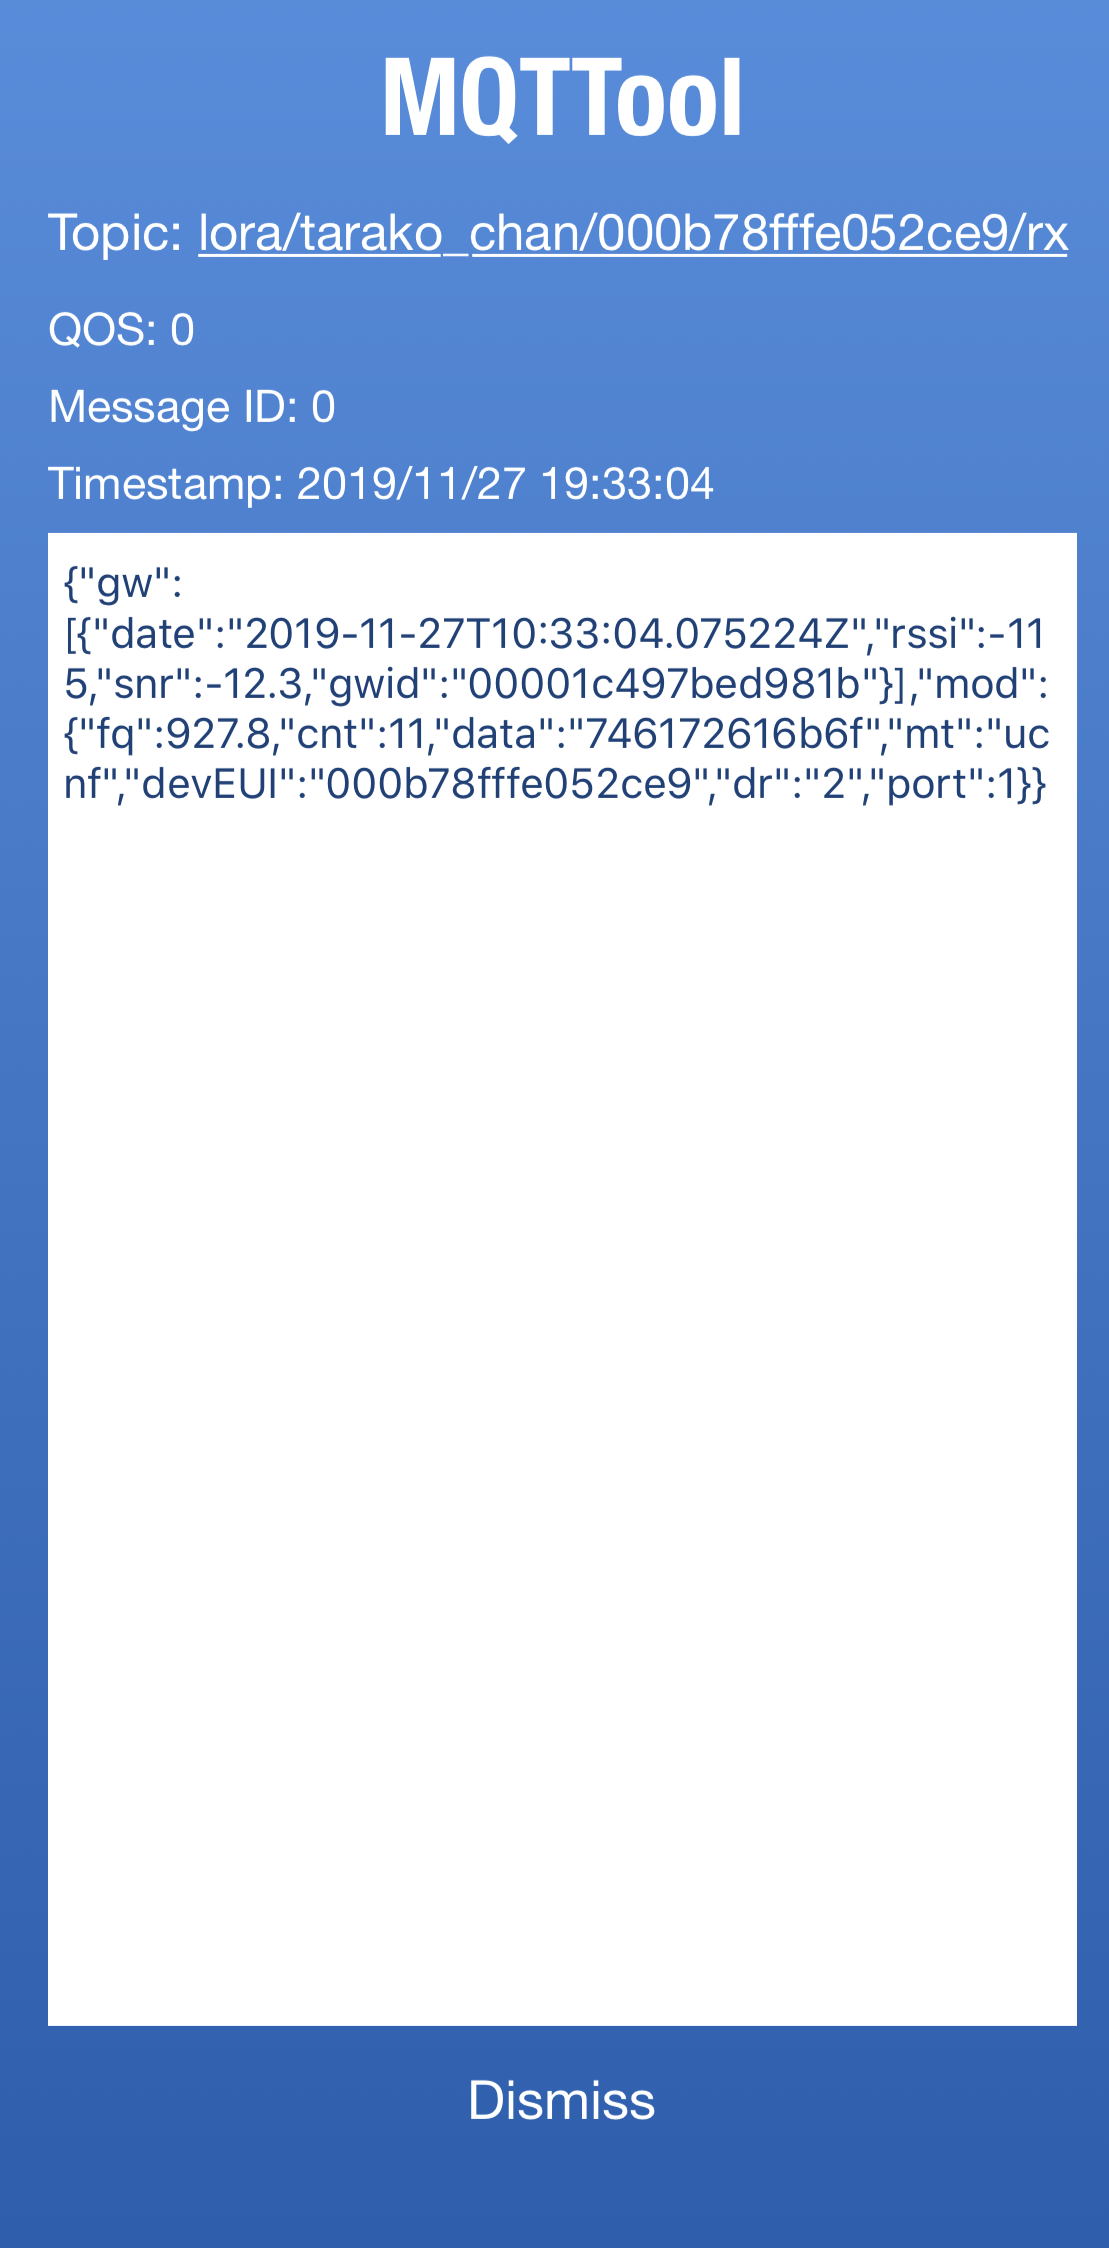
\includegraphics[width=5cm]{figures/mqtt.PNG}
    \caption{MQTT Client}
    \label{fig:mqtt}
    \end{center}
\end{figure}

\begin{figure}[]
    \begin{center}
    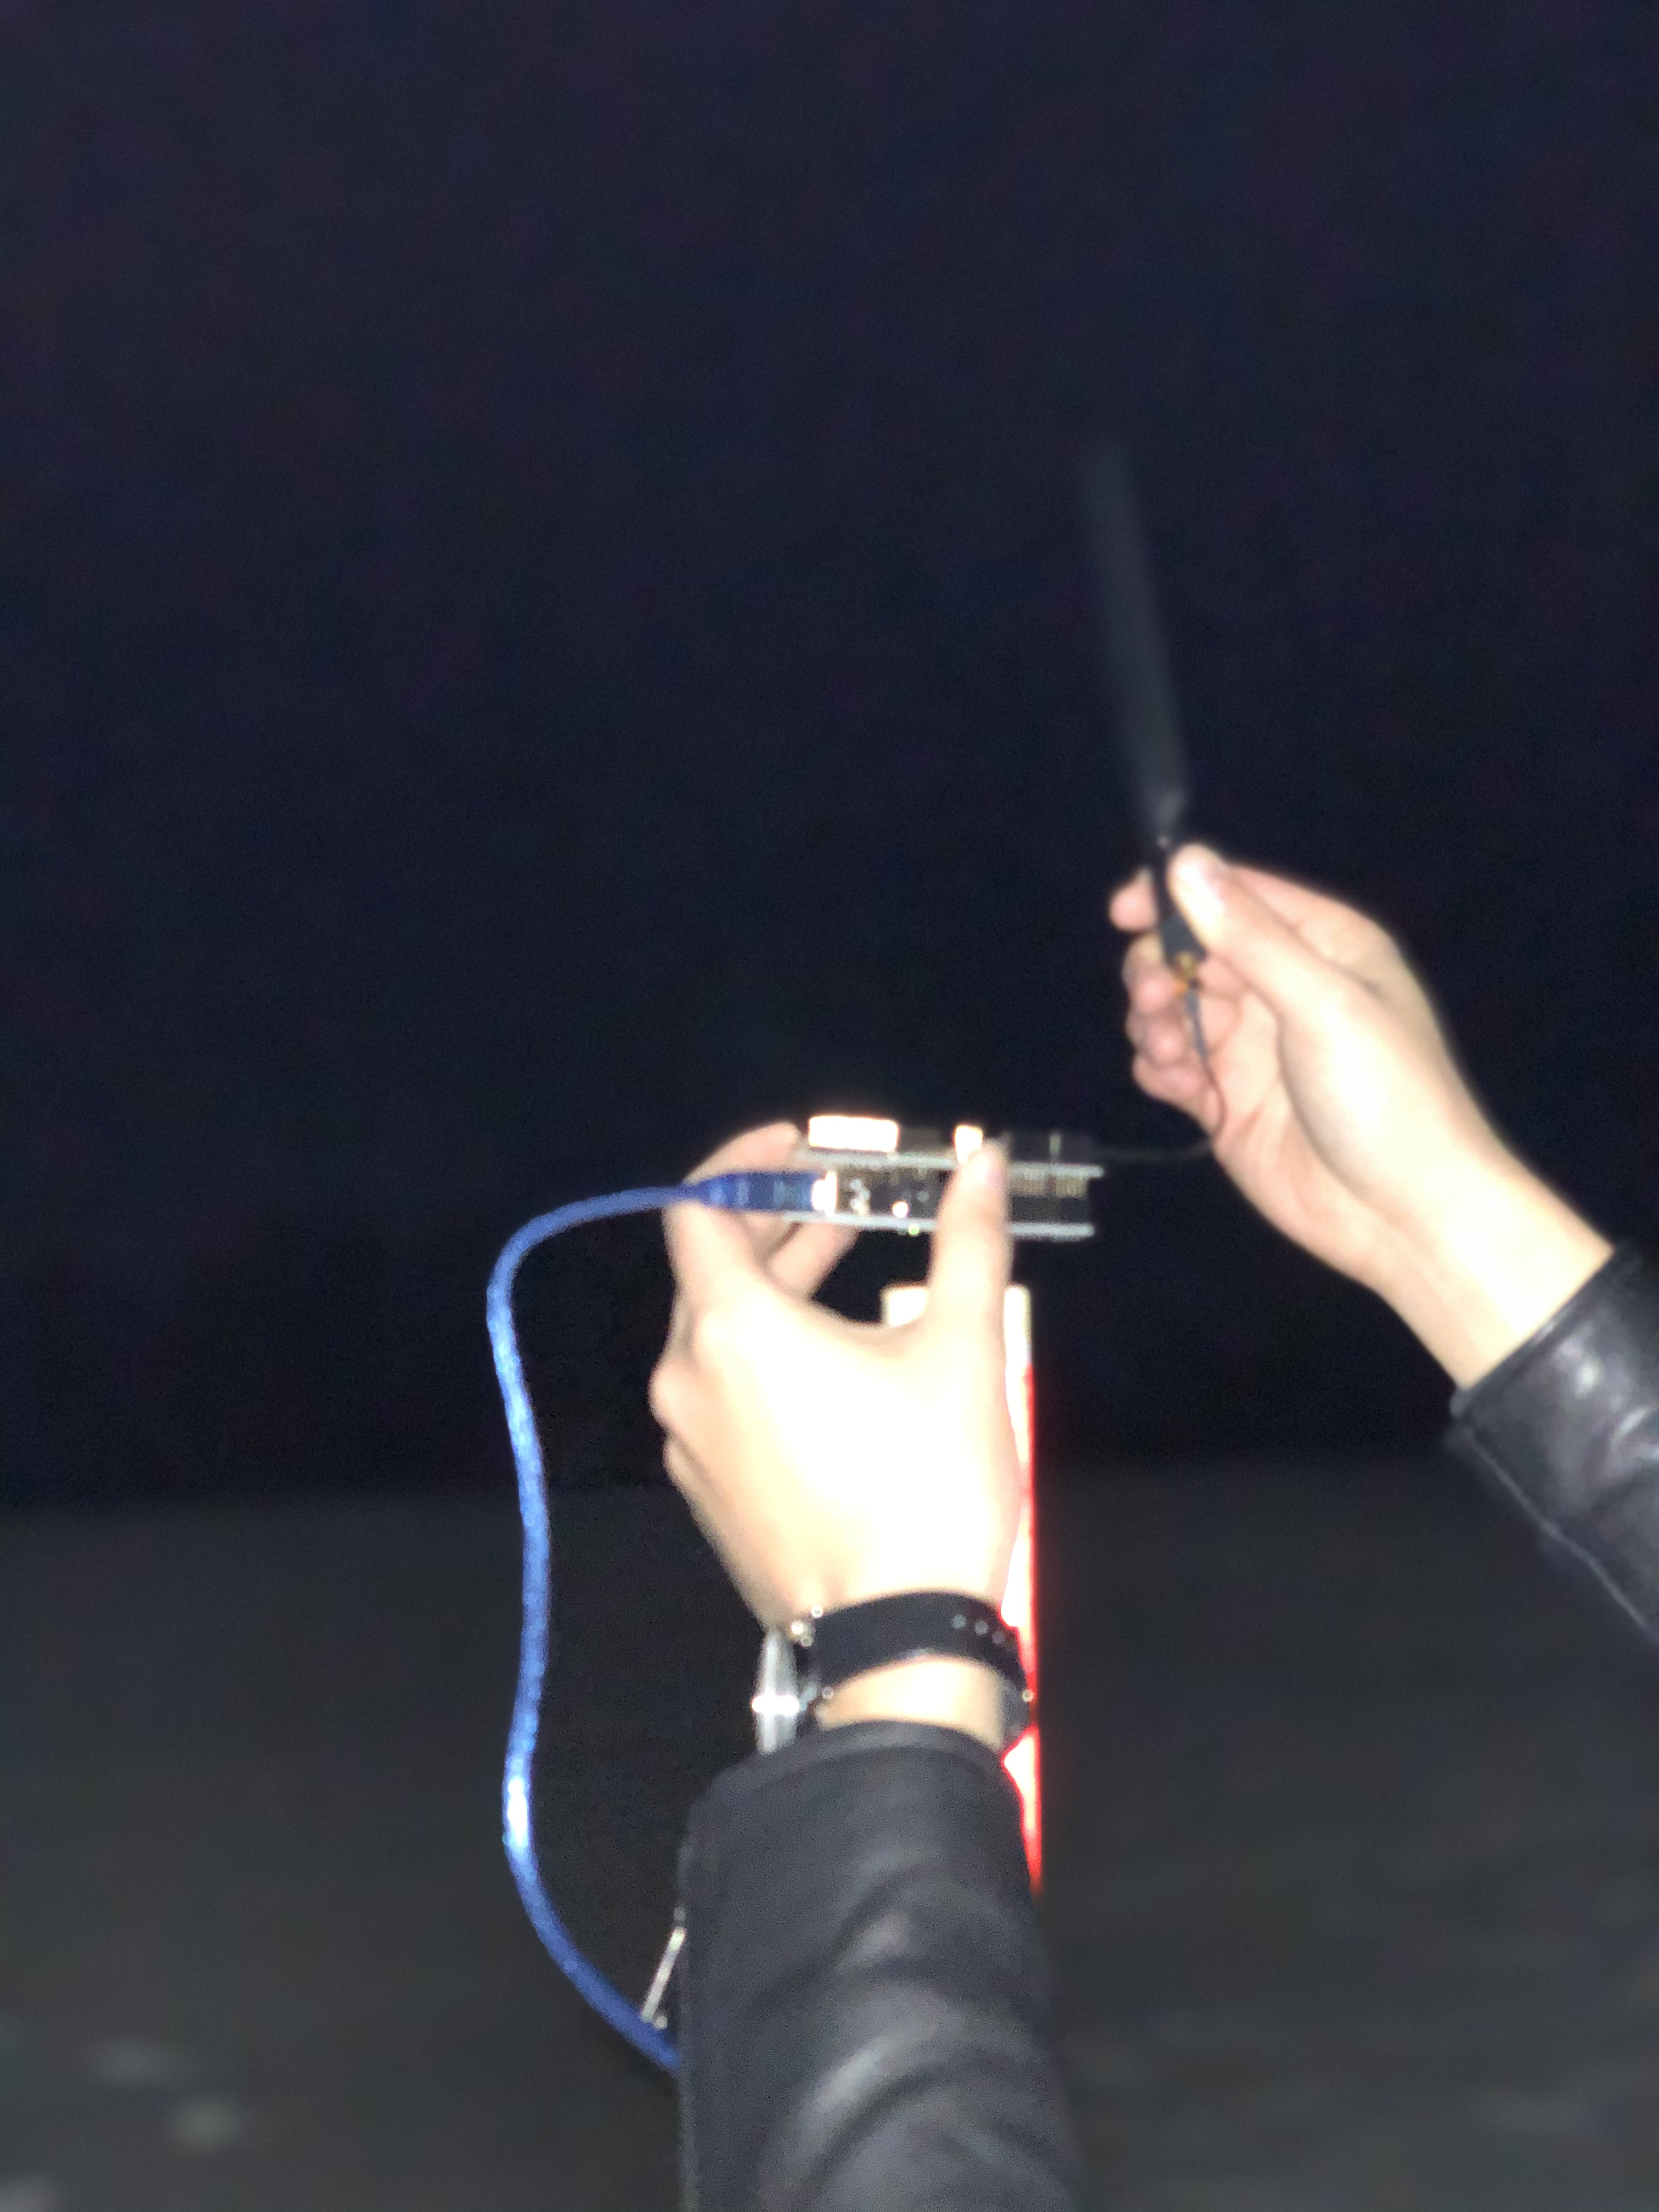
\includegraphics[width=5cm]{figures/experiment.jpg}
    \caption{実測実験の様子}
    \label{fig:experiment}
    \end{center}
\end{figure}

% ----
\section{実験結果}
LoRaWAN (DR2)でのイベントごとの消費電力実測結果を下記(表\ref{fig:result_power_consumtion}参照)(表\ref{fig:LoRaWAN_PowerConsumption}参照)に示す.また,LoRaWAN (DR2)でのその他値を下記(表\ref{fig:LoRaWAN_Parameter}参照)に示す.パケット到達率は,LoRaWANの送信回数に対してMQTTブローカーで受信したデータ数をもとに算出した.RSSiは,LoRaWANのGWノードが収集しMQTTブローカーに送信するため,その値を参考とした.SNRも同様である.

\begin{figure}[]
    \begin{center}
    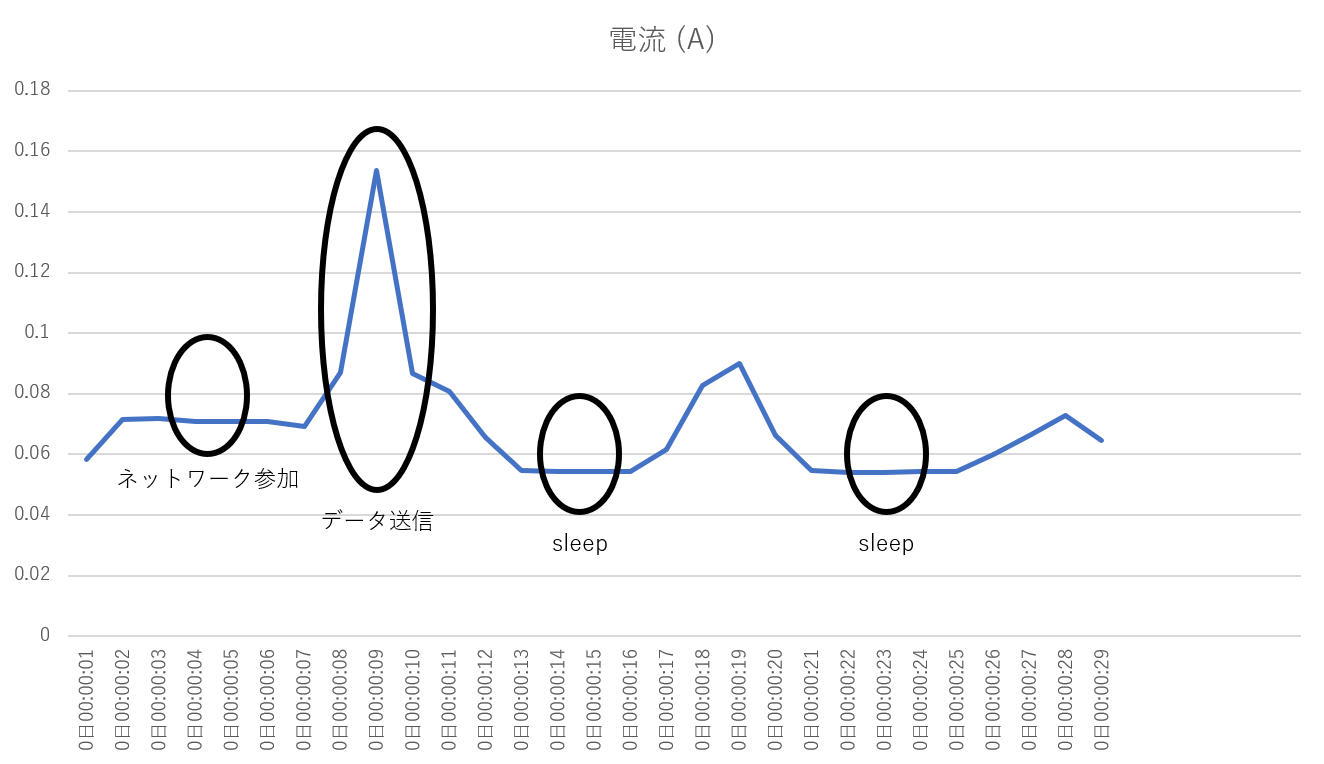
\includegraphics[width=15cm]{figures/LoRaWAN_消費電力実験.png}
    \caption{消費電力測定における各イベント(縦軸:消費電流,横軸:時間(s))}
    \label{fig:result_power_consumtion}
    \end{center}
\end{figure}

\begin{table}[]
    \caption{イベントごとの消費電力}\label{fig:LoRaWAN_PowerConsumption}
    \centering
    \begin{tabular}{|c|l|l|l|}
    \hline
    \textbf{イベント}     & \multicolumn{1}{c|}{\textbf{時間 (second)}} & \multicolumn{1}{c|}{\textbf{電流 (mA)}} & \multicolumn{1}{c|}{\textbf{消費電力 (mW)}} \\ \hline
    起動→ネットワーク参加       & 7                                         & 20                                    & 120                                     \\ \hline
    起動→ネットワーク参加→データ送信 & 11                                        & 21                                    & 105                                     \\ \hline
    スリープ              & なし                                        & 3                                     & 15                                      \\ \hline
    データ送信             & 4                                         & 29                                    & 145                                     \\ \hline
    \end{tabular}
\end{table}

\begin{table}[]
    \caption{その他パラメータ}\label{fig:LoRaWAN_Parameter}
    \centering
    \begin{tabular}{|c|c|}
    \hline
    \textbf{パラメータ} & \textbf{値} \\ \hline
    パケット到達率        & 90\%       \\ \hline
    RSSi           & -102       \\ \hline
    SNR            & -10        \\ \hline
    \end{tabular}
\end{table}
% % --- 関連技術 ---
% \chapter{実測に基づくグループ化アルゴリズムの適応点の評価}

\section{実験目的}
% 何を評価するために何を測って,どうなるとOKか,まで書いてください.
前項5.1.3(グループ化アルゴリズムの適応点の検討)で述べたように,グループ化の適応点を明らかにするため,LoRaWANにおける消費電力の実測を行う.適応点の評価については,前述したLoRaWANの既存方式と提案手法における関係式5.3に,実測した値を代入することで判断する.

\section{実験方法}
提案システムにおける各シーケンスにおいて消費電力を求めるため,起動からネットワーク参加,起動からネットワーク参加・初回送信,定常時の送信,スリープとイベントごと消費電力を計測する必要がある.実験では,市販のArduino互換LoRaWANモジュール及び消費電力計を用いて,消費電力を計測した.実験環境は,下記の表に示す.実験機材は,LoRaWANの送信機に,シングルボードコンピューターであるArduino Uno R3(表\ref{fig:Arduino_Spec}参照),LoRaWAN Shield for Arduino\cite{lorashield}(表\ref{fig:LoRaWAN_Spec}参照),受信機にLoRaWAN Gateway\cite{loragateway}(表\ref{fig:LoRaWAN_Gateway_Spec}),消費電力測定にマルチメータ\cite{kotomi}(表\ref{fig:Kotomi_Spec}参照)を用いた.LoRaWANは長距離伝送がユースケースであるため,LoRaWANのノードとGWノードを,高低差があり,約3.5kmの距離がある公立はこだて未来大学と自宅間に配置した.また計測結果を保存できる容量に限りがあるため,3試行を1セットとした.LoRaWANの設定内容を述べる.前述したLoRaWANのADR機能を適応し,スリープ時間は4秒とした.30秒間の計測を4セット12試行した.パケット到達率を算出するため,データ受信を確認する必要がある.本実測で利用したLoRaWANモジュールのプロバイダーは,MQTT ブローカーが提供しているため,MQTT クライアント\cite{mqtttool}を用いてデータを取得した.下記(図\ref{fig:experiment}参照)は,実験の様子である.

\begin{table}[]
    \caption{ARDUINO UNO REV3}\label{fig:Arduino_Spec}
    \centering
    \begin{tabular}{|c|c|}
    \hline
    動作電圧     & 5V   \\ \hline
    DC電流     & 50mA \\ \hline
    フラッシュメモリ & 32KB \\ \hline
    SRAM     & 2KB  \\ \hline
    EEPROM   & 1KB  \\ \hline
    \end{tabular}
\end{table}

\begin{table}[]
    \caption{LoRaWAN Shield for Arduino}\label{fig:LoRaWAN_Spec}
    \centering
    \begin{tabular}{|c|c|}
    \hline
    電源電圧 & DC2.2 $\sim$3.6V      \\ \hline
    周波数  & 920.6MHz $\sim$928MHz \\ \hline
    動作温度 & 0°C $\sim$40 °C       \\ \hline
    サイズ  & 68mm×53mm × 22.8mm    \\ \hline
    無線規格 & LoRaWAN 1.0.2         \\ \hline
    \end{tabular}
\end{table}

\begin{table}[]
    \caption{Kotomi Premium}\label{fig:Kotomi_Spec}
    \centering
    \begin{tabular}{|l|l|}
    \hline
    サイズ    & 77 x 35 x 13mm \\ \hline
    ディスプレイ & 1.44インチ        \\ \hline
    電圧精度   & 0.0001V        \\ \hline
    電流制度   & 0.0001A        \\ \hline
    電圧範囲   & 3.7~25V        \\ \hline
    電流範囲   & 0~5A           \\ \hline
    \end{tabular}
\end{table}

\begin{table}[]
    \caption{LoRaWAN Gateway}\label{fig:LoRaWAN_Gateway_Spec}
    \centering
    \begin{tabular}{|c|c|}
    \hline
    モデル名         & SW-GW01                       \\ \hline
    チャンネル数       & 最大8ch                         \\ \hline
    Wireless LAN & 802.11 b/g/n 2.4G             \\ \hline
    送信出力         & 20mW (最大13 dBm)               \\ \hline
    受信感度         & Down to -142 dBm              \\ \hline
    動作温度         & -10ºC $\sim$55ºC              \\ \hline
    電源電圧         & DC 5V / 2A(ミニUSBポート経由)        \\ \hline
    インターフェース     & Ethernet x 1ポート, 3/4G USBドングル \\ \hline
    サイズ          & L:116 x W:91 x H:27 mm        \\ \hline
    重量           & 160g                          \\ \hline
    \end{tabular}
\end{table}

\begin{table}[]
    \caption{実測に用いた電源}\label{fig:LoRaWAN_Battery}
    \centering
    \begin{tabular}{|c|c|}
    \hline
    サイズ     & 72 x 70 x 31 (mm) \\ \hline
    重量      & 189g              \\ \hline
    バッテリー容量 & 5000mAh           \\ \hline
    入力      & 5V=2A             \\ \hline
    出力      & 5V=3A             \\ \hline
    \end{tabular}
\end{table}

\begin{figure}[]
    \begin{center}
    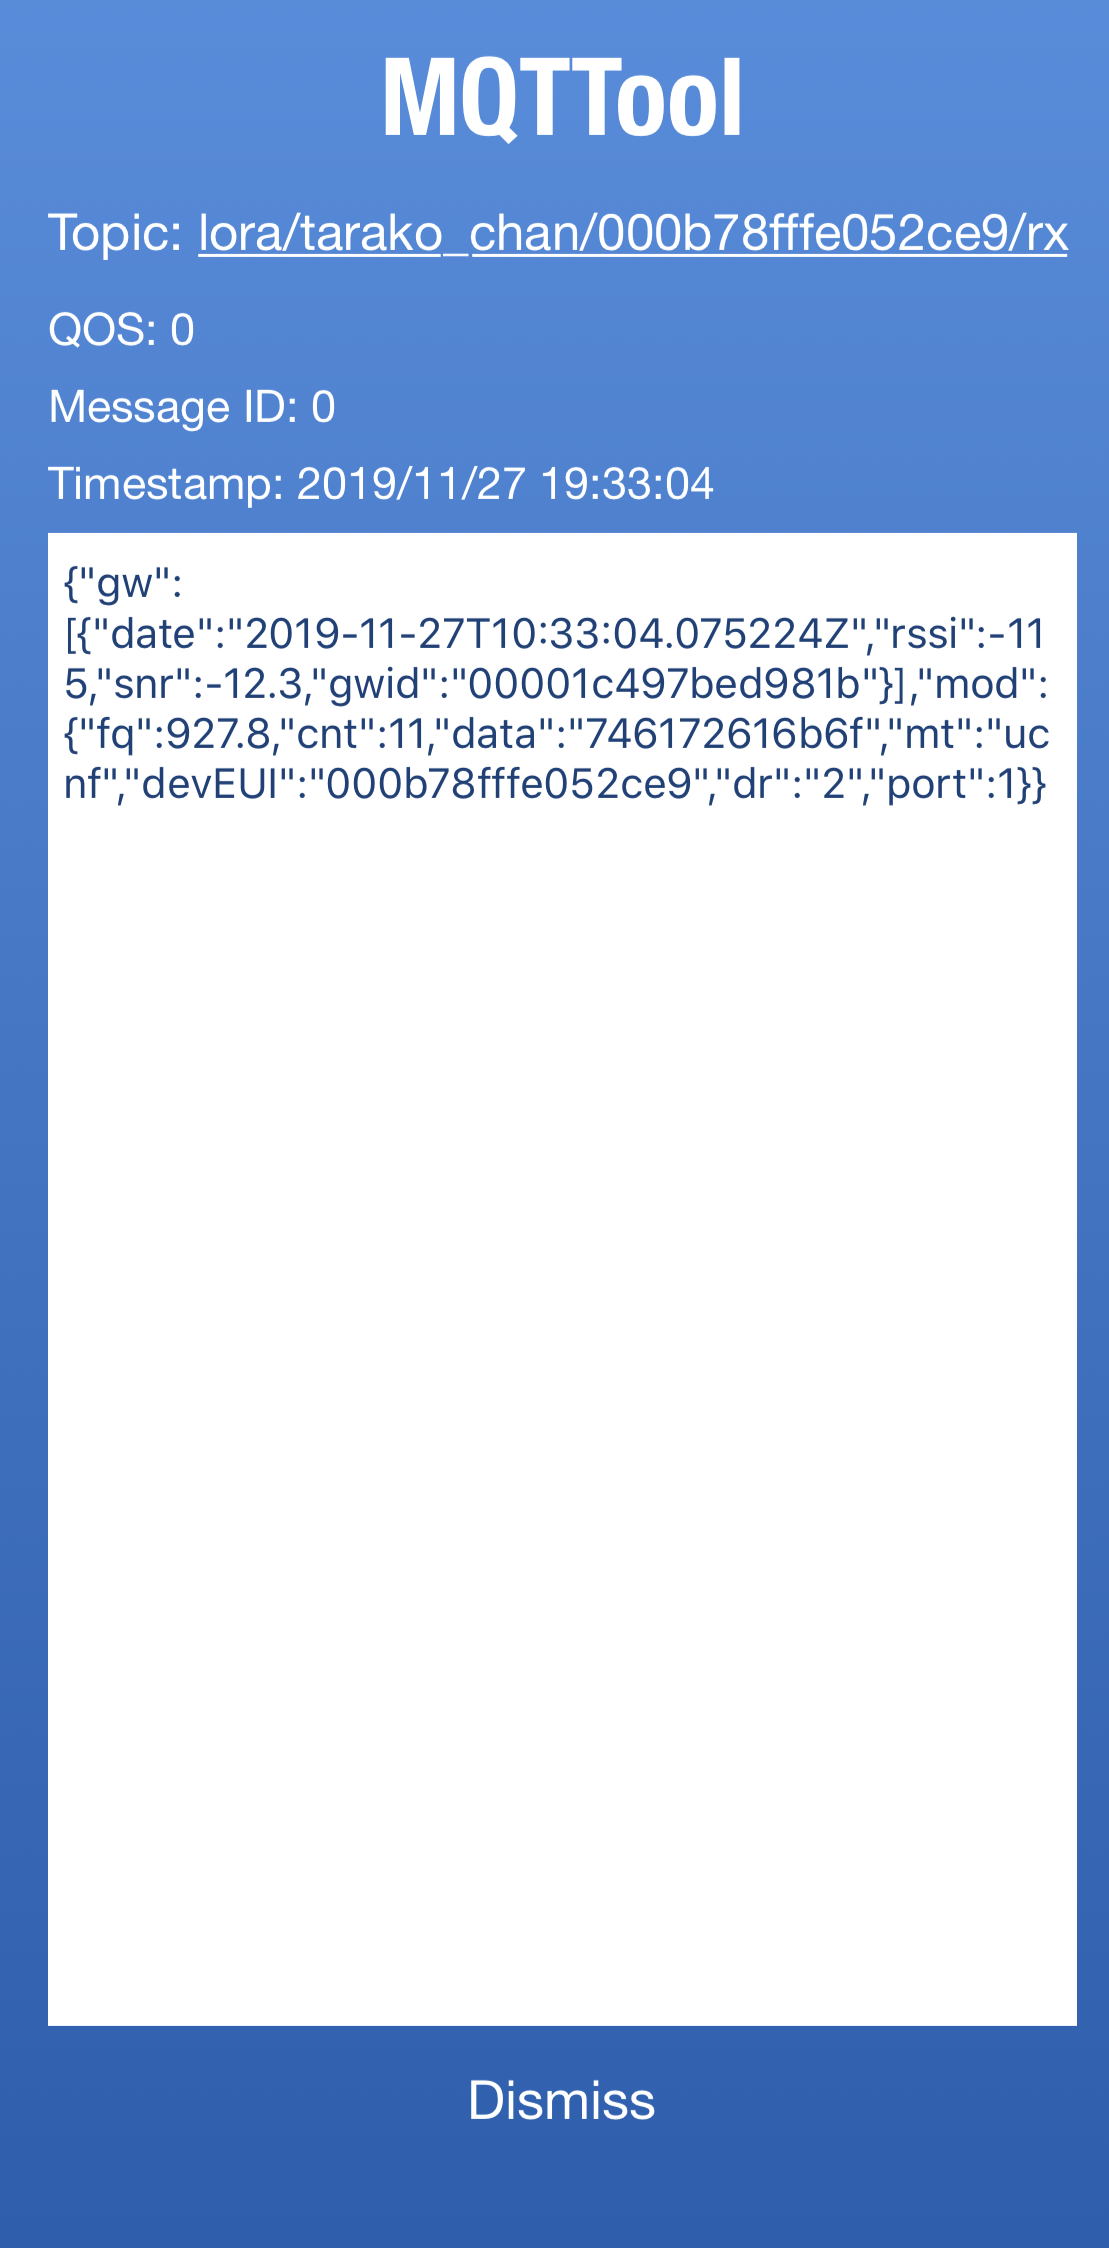
\includegraphics[width=5cm]{figures/mqtt.PNG}
    \caption{MQTT Client}
    \label{fig:mqtt}
    \end{center}
\end{figure}

\begin{figure}[]
    \begin{center}
    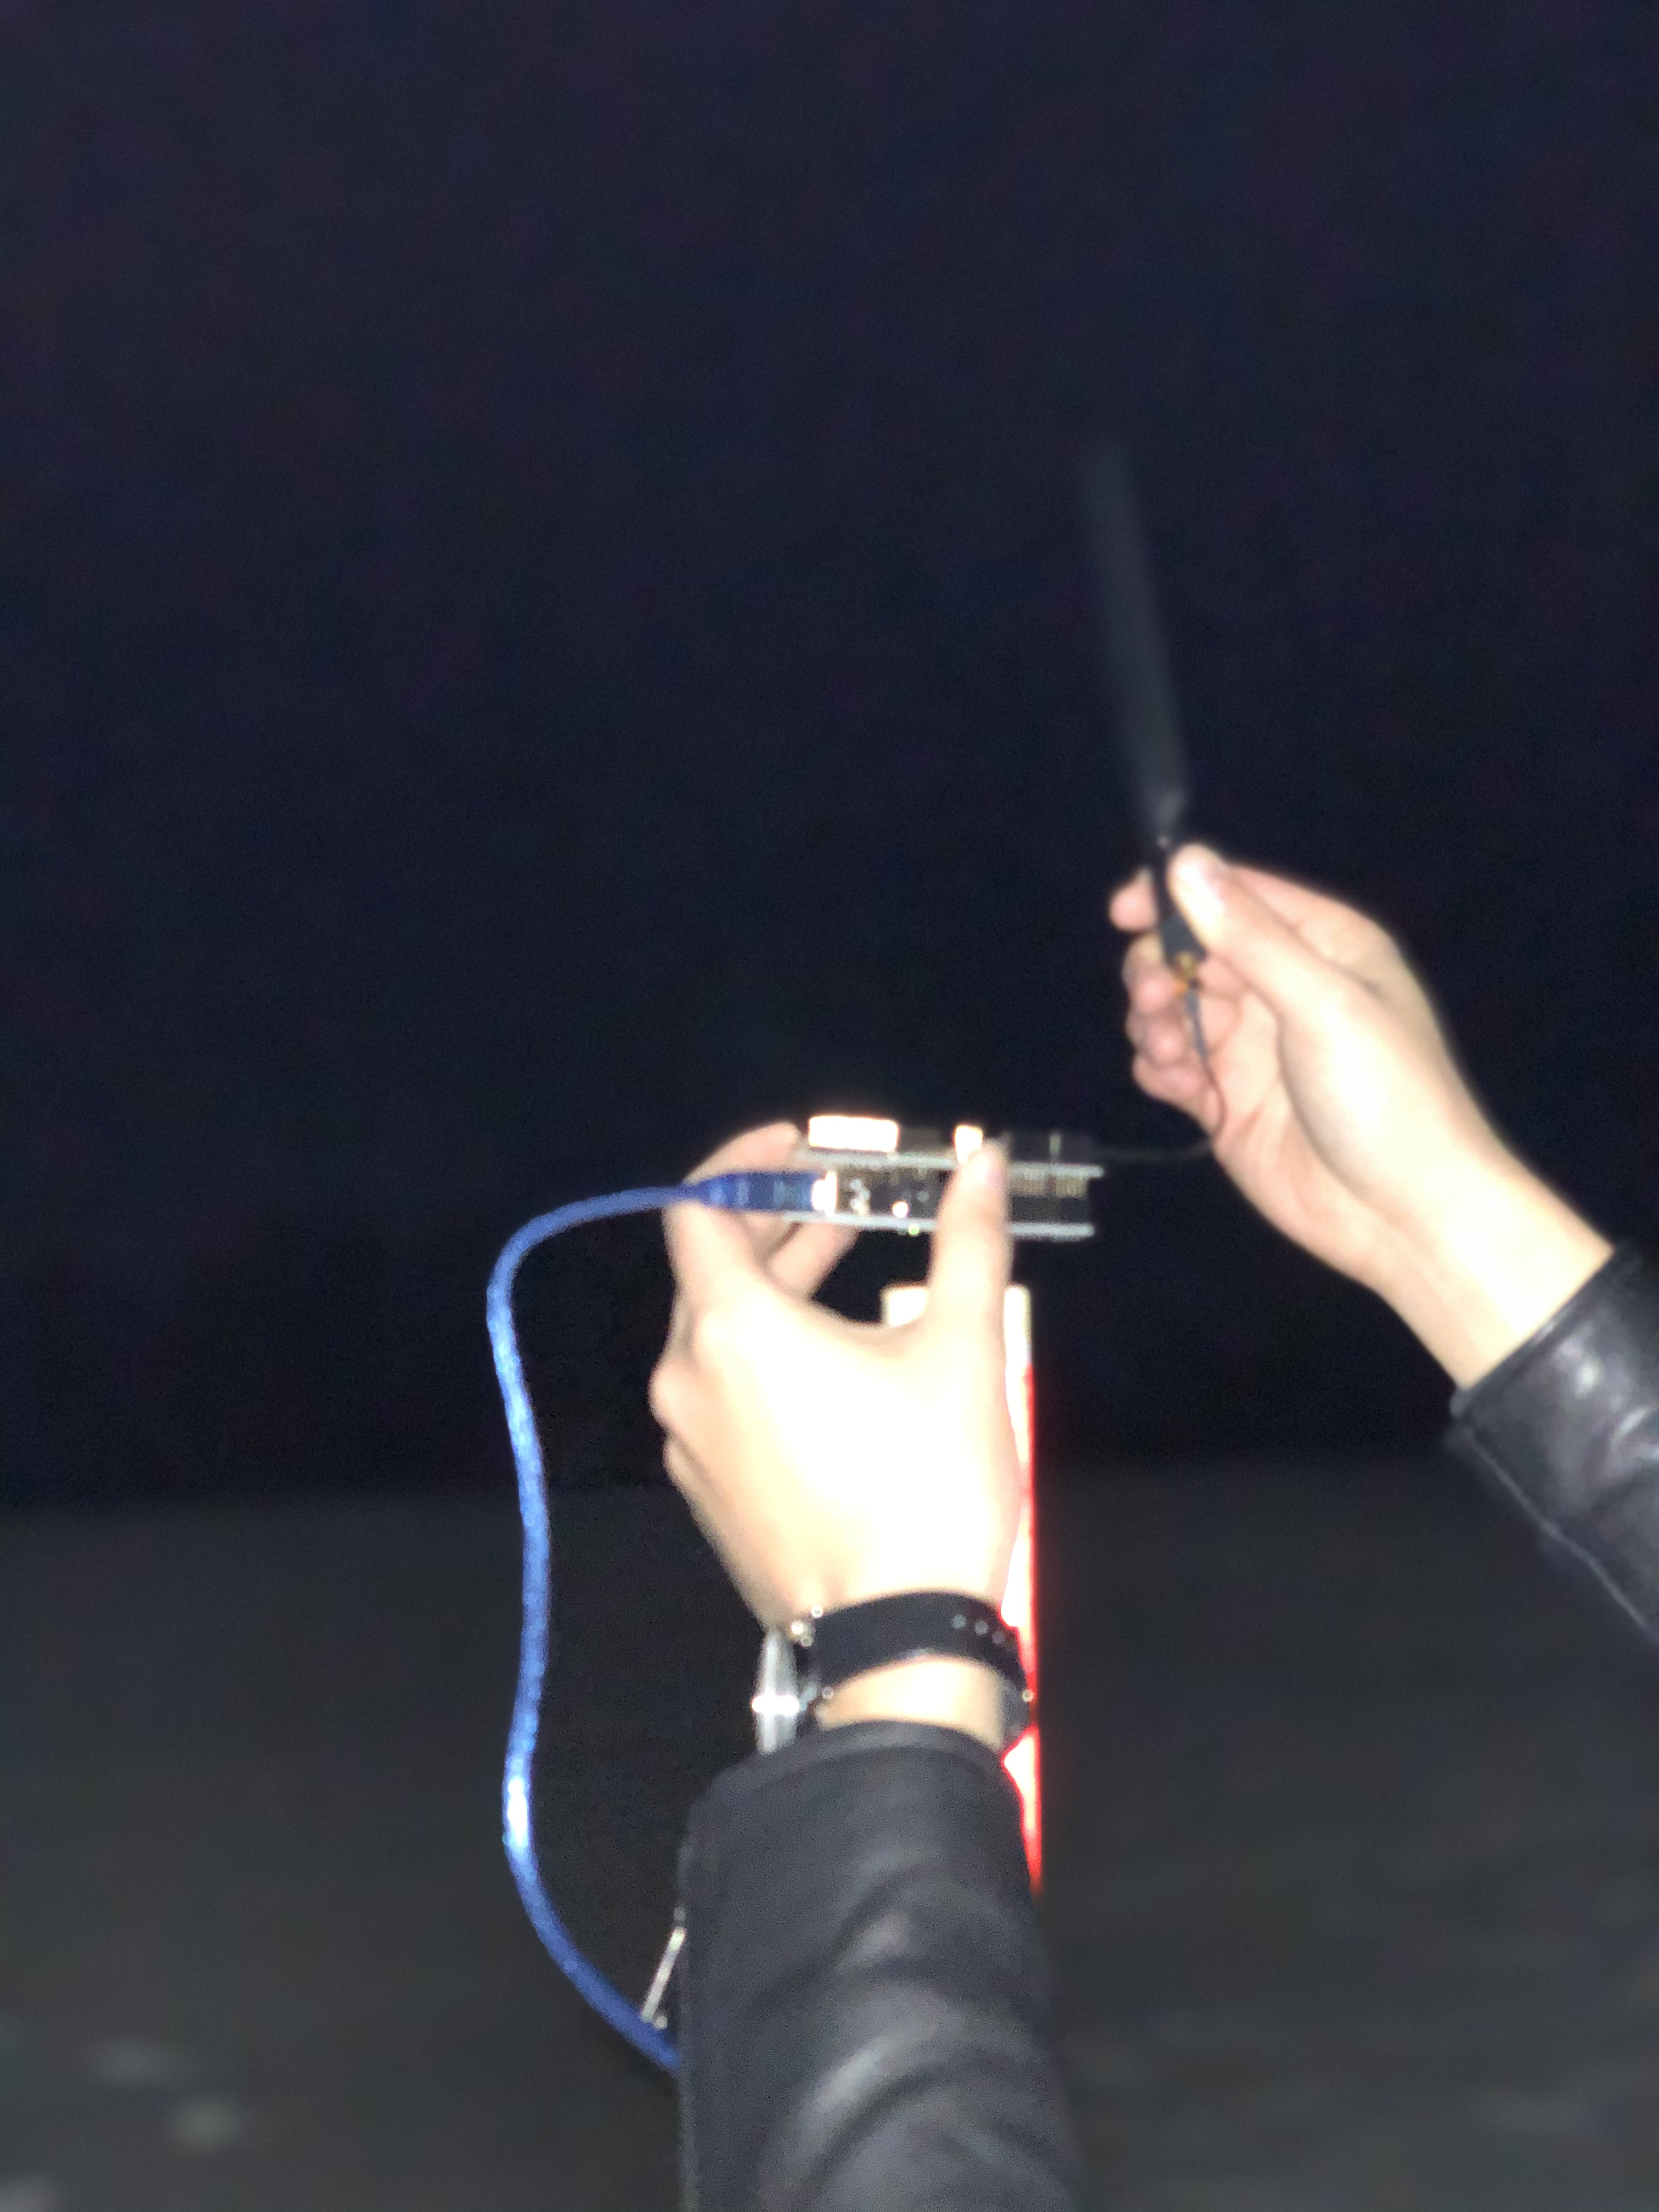
\includegraphics[width=5cm]{figures/experiment.jpg}
    \caption{実測実験の様子}
    \label{fig:experiment}
    \end{center}
\end{figure}

% ----
\section{実験結果}
LoRaWAN (DR2)でのイベントごとの消費電力実測結果を下記(表\ref{fig:result_power_consumtion}参照)(表\ref{fig:LoRaWAN_PowerConsumption}参照)に示す.また,LoRaWAN (DR2)でのその他値を下記(表\ref{fig:LoRaWAN_Parameter}参照)に示す.パケット到達率は,LoRaWANの送信回数に対してMQTTブローカーで受信したデータ数をもとに算出した.RSSiは,LoRaWANのGWノードが収集しMQTTブローカーに送信するため,その値を参考とした.SNRも同様である.

\begin{figure}[]
    \begin{center}
    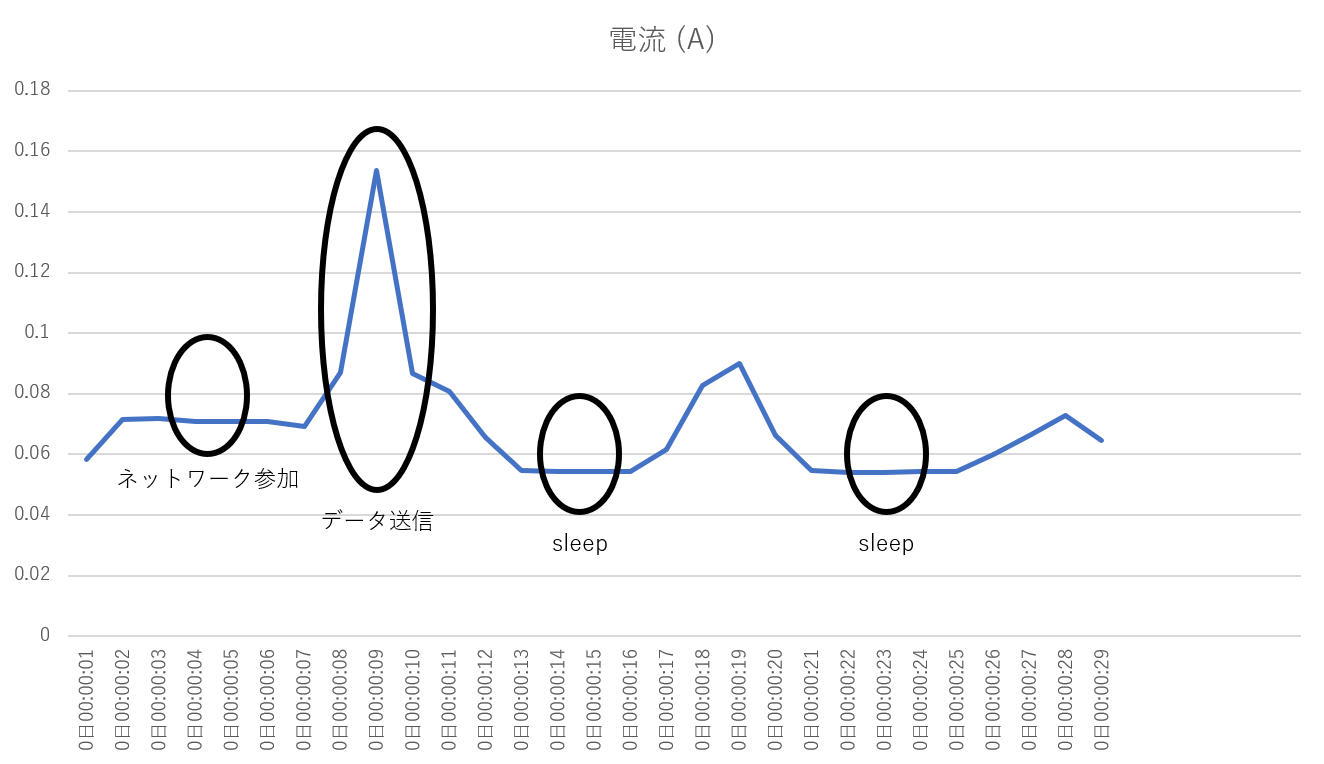
\includegraphics[width=15cm]{figures/LoRaWAN_消費電力実験.png}
    \caption{消費電力測定における各イベント(縦軸:消費電流,横軸:時間(s))}
    \label{fig:result_power_consumtion}
    \end{center}
\end{figure}

\begin{table}[]
    \caption{イベントごとの消費電力}\label{fig:LoRaWAN_PowerConsumption}
    \centering
    \begin{tabular}{|c|l|l|l|}
    \hline
    \textbf{イベント}     & \multicolumn{1}{c|}{\textbf{時間 (second)}} & \multicolumn{1}{c|}{\textbf{電流 (mA)}} & \multicolumn{1}{c|}{\textbf{消費電力 (mW)}} \\ \hline
    起動→ネットワーク参加       & 7                                         & 20                                    & 120                                     \\ \hline
    起動→ネットワーク参加→データ送信 & 11                                        & 21                                    & 105                                     \\ \hline
    スリープ              & なし                                        & 3                                     & 15                                      \\ \hline
    データ送信             & 4                                         & 29                                    & 145                                     \\ \hline
    \end{tabular}
\end{table}

\begin{table}[]
    \caption{その他パラメータ}\label{fig:LoRaWAN_Parameter}
    \centering
    \begin{tabular}{|c|c|}
    \hline
    \textbf{パラメータ} & \textbf{値} \\ \hline
    パケット到達率        & 90\%       \\ \hline
    RSSi           & -102       \\ \hline
    SNR            & -10        \\ \hline
    \end{tabular}
\end{table}
% % --- 関連研究 ---
% \chapter{実測に基づくグループ化アルゴリズムの適応点の評価}

\section{実験目的}
% 何を評価するために何を測って,どうなるとOKか,まで書いてください.
前項5.1.3(グループ化アルゴリズムの適応点の検討)で述べたように,グループ化の適応点を明らかにするため,LoRaWANにおける消費電力の実測を行う.適応点の評価については,前述したLoRaWANの既存方式と提案手法における関係式5.3に,実測した値を代入することで判断する.

\section{実験方法}
提案システムにおける各シーケンスにおいて消費電力を求めるため,起動からネットワーク参加,起動からネットワーク参加・初回送信,定常時の送信,スリープとイベントごと消費電力を計測する必要がある.実験では,市販のArduino互換LoRaWANモジュール及び消費電力計を用いて,消費電力を計測した.実験環境は,下記の表に示す.実験機材は,LoRaWANの送信機に,シングルボードコンピューターであるArduino Uno R3(表\ref{fig:Arduino_Spec}参照),LoRaWAN Shield for Arduino\cite{lorashield}(表\ref{fig:LoRaWAN_Spec}参照),受信機にLoRaWAN Gateway\cite{loragateway}(表\ref{fig:LoRaWAN_Gateway_Spec}),消費電力測定にマルチメータ\cite{kotomi}(表\ref{fig:Kotomi_Spec}参照)を用いた.LoRaWANは長距離伝送がユースケースであるため,LoRaWANのノードとGWノードを,高低差があり,約3.5kmの距離がある公立はこだて未来大学と自宅間に配置した.また計測結果を保存できる容量に限りがあるため,3試行を1セットとした.LoRaWANの設定内容を述べる.前述したLoRaWANのADR機能を適応し,スリープ時間は4秒とした.30秒間の計測を4セット12試行した.パケット到達率を算出するため,データ受信を確認する必要がある.本実測で利用したLoRaWANモジュールのプロバイダーは,MQTT ブローカーが提供しているため,MQTT クライアント\cite{mqtttool}を用いてデータを取得した.下記(図\ref{fig:experiment}参照)は,実験の様子である.

\begin{table}[]
    \caption{ARDUINO UNO REV3}\label{fig:Arduino_Spec}
    \centering
    \begin{tabular}{|c|c|}
    \hline
    動作電圧     & 5V   \\ \hline
    DC電流     & 50mA \\ \hline
    フラッシュメモリ & 32KB \\ \hline
    SRAM     & 2KB  \\ \hline
    EEPROM   & 1KB  \\ \hline
    \end{tabular}
\end{table}

\begin{table}[]
    \caption{LoRaWAN Shield for Arduino}\label{fig:LoRaWAN_Spec}
    \centering
    \begin{tabular}{|c|c|}
    \hline
    電源電圧 & DC2.2 $\sim$3.6V      \\ \hline
    周波数  & 920.6MHz $\sim$928MHz \\ \hline
    動作温度 & 0°C $\sim$40 °C       \\ \hline
    サイズ  & 68mm×53mm × 22.8mm    \\ \hline
    無線規格 & LoRaWAN 1.0.2         \\ \hline
    \end{tabular}
\end{table}

\begin{table}[]
    \caption{Kotomi Premium}\label{fig:Kotomi_Spec}
    \centering
    \begin{tabular}{|l|l|}
    \hline
    サイズ    & 77 x 35 x 13mm \\ \hline
    ディスプレイ & 1.44インチ        \\ \hline
    電圧精度   & 0.0001V        \\ \hline
    電流制度   & 0.0001A        \\ \hline
    電圧範囲   & 3.7~25V        \\ \hline
    電流範囲   & 0~5A           \\ \hline
    \end{tabular}
\end{table}

\begin{table}[]
    \caption{LoRaWAN Gateway}\label{fig:LoRaWAN_Gateway_Spec}
    \centering
    \begin{tabular}{|c|c|}
    \hline
    モデル名         & SW-GW01                       \\ \hline
    チャンネル数       & 最大8ch                         \\ \hline
    Wireless LAN & 802.11 b/g/n 2.4G             \\ \hline
    送信出力         & 20mW (最大13 dBm)               \\ \hline
    受信感度         & Down to -142 dBm              \\ \hline
    動作温度         & -10ºC $\sim$55ºC              \\ \hline
    電源電圧         & DC 5V / 2A(ミニUSBポート経由)        \\ \hline
    インターフェース     & Ethernet x 1ポート, 3/4G USBドングル \\ \hline
    サイズ          & L:116 x W:91 x H:27 mm        \\ \hline
    重量           & 160g                          \\ \hline
    \end{tabular}
\end{table}

\begin{table}[]
    \caption{実測に用いた電源}\label{fig:LoRaWAN_Battery}
    \centering
    \begin{tabular}{|c|c|}
    \hline
    サイズ     & 72 x 70 x 31 (mm) \\ \hline
    重量      & 189g              \\ \hline
    バッテリー容量 & 5000mAh           \\ \hline
    入力      & 5V=2A             \\ \hline
    出力      & 5V=3A             \\ \hline
    \end{tabular}
\end{table}

\begin{figure}[]
    \begin{center}
    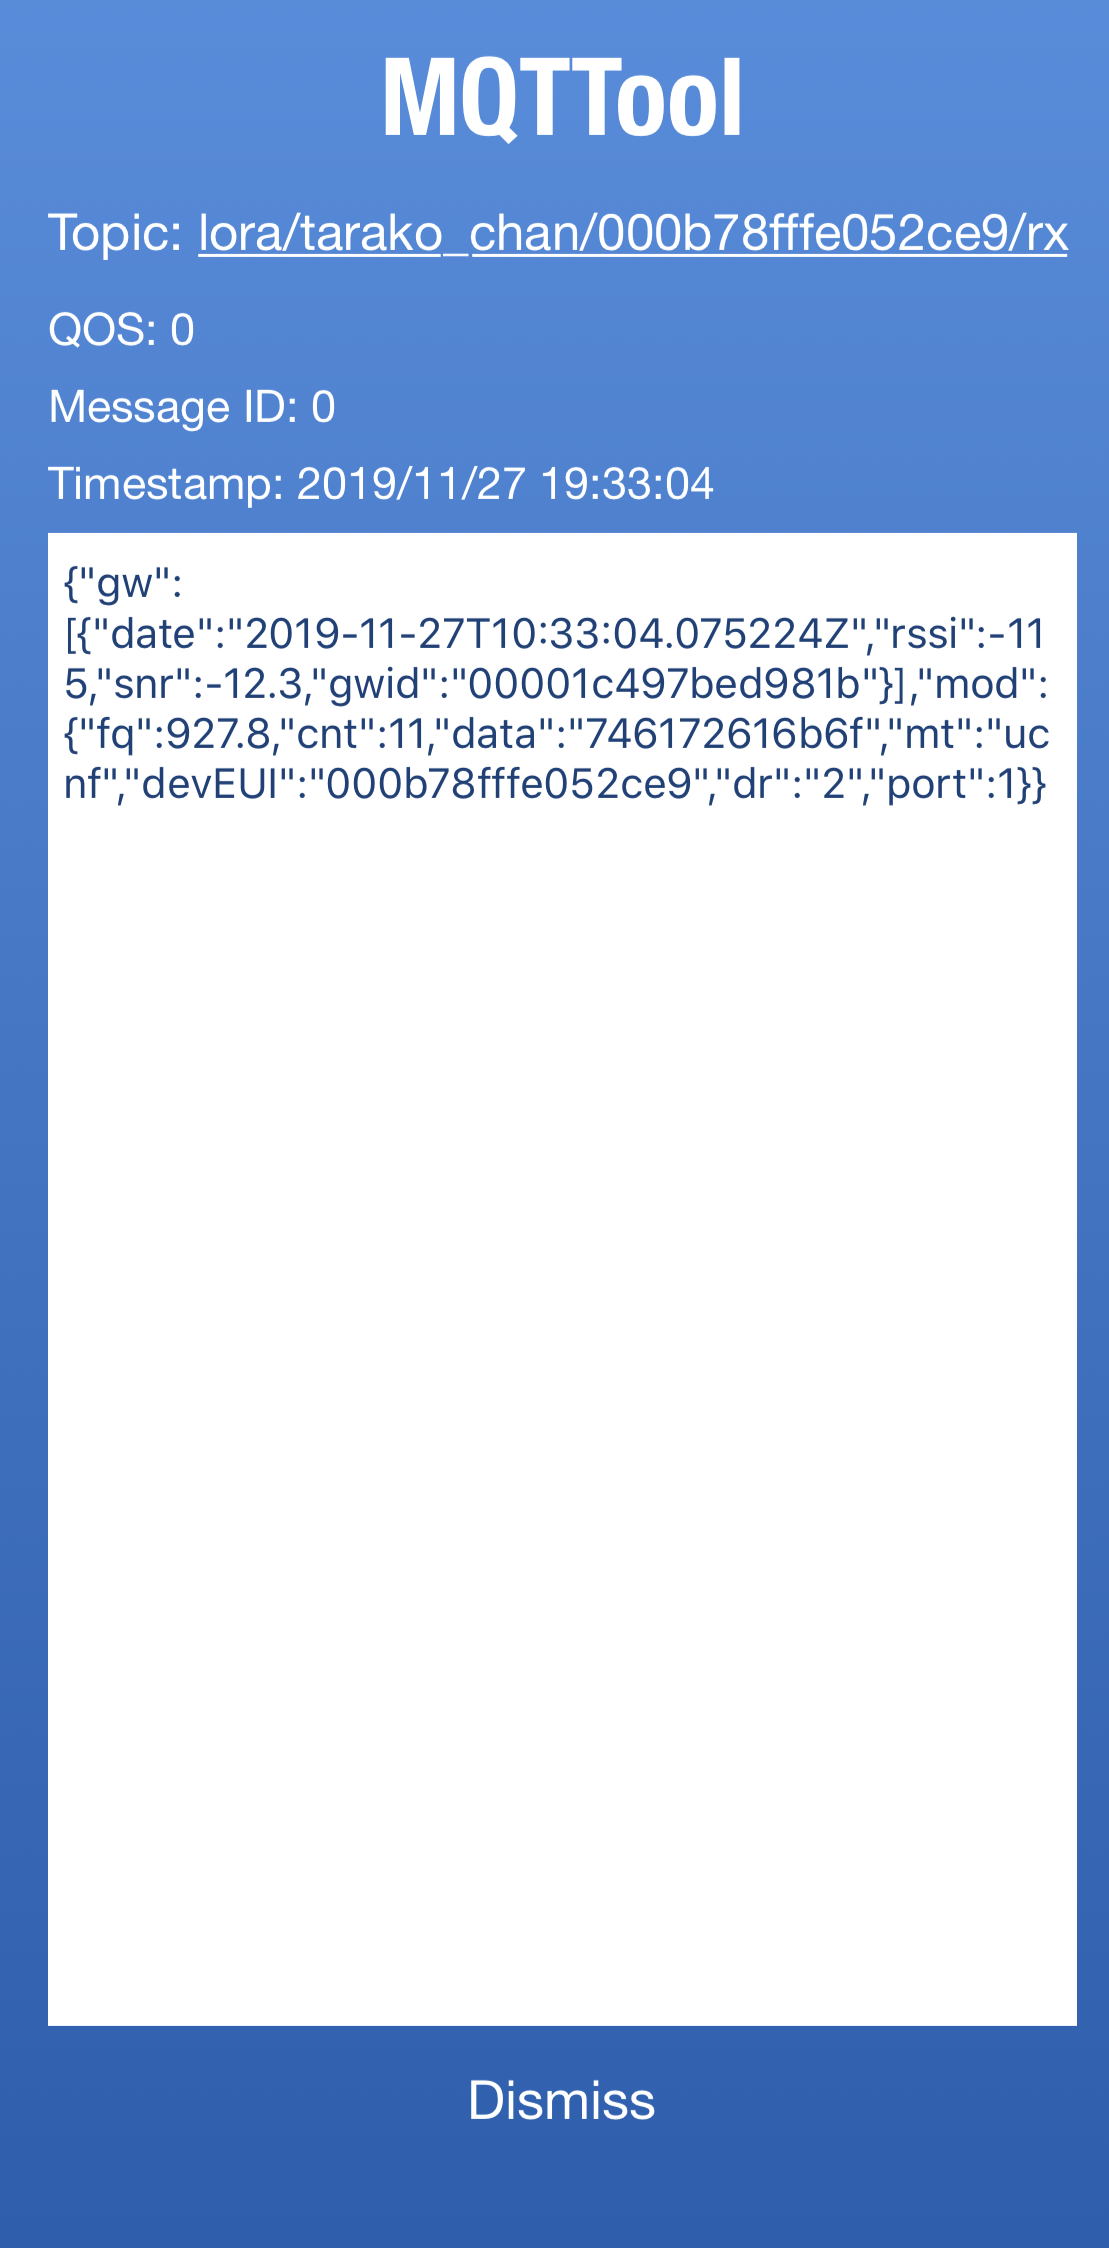
\includegraphics[width=5cm]{figures/mqtt.PNG}
    \caption{MQTT Client}
    \label{fig:mqtt}
    \end{center}
\end{figure}

\begin{figure}[]
    \begin{center}
    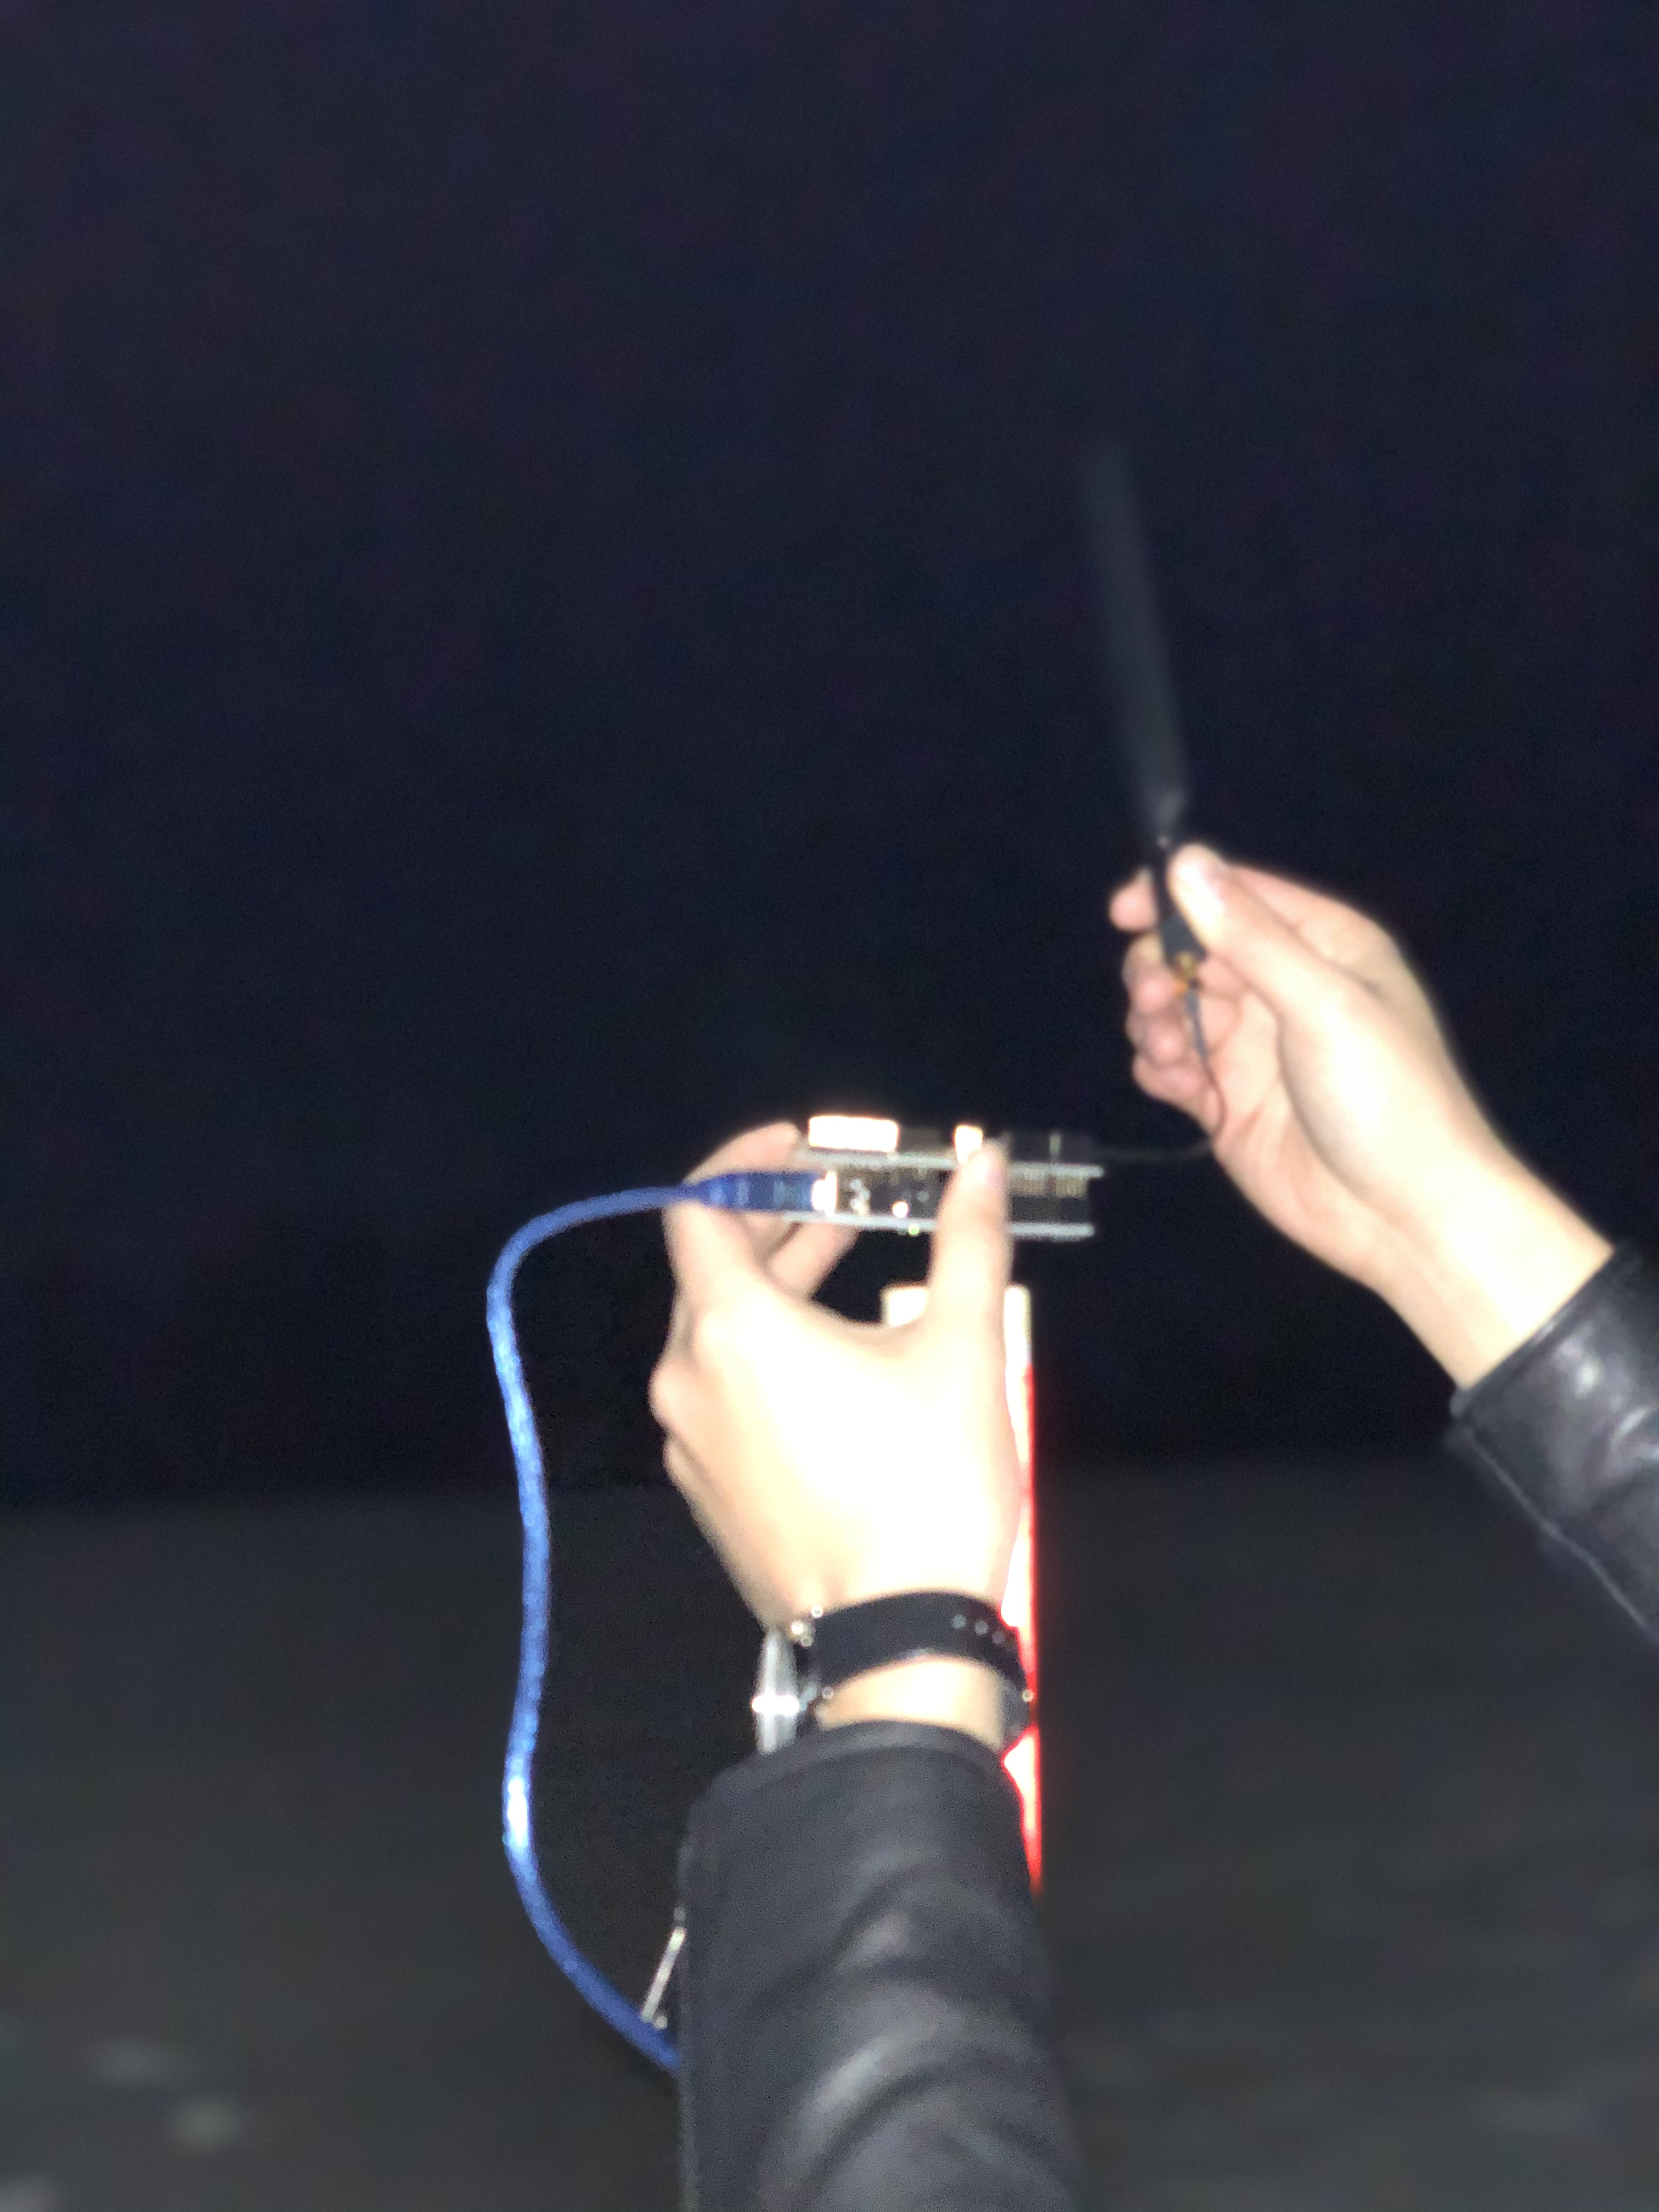
\includegraphics[width=5cm]{figures/experiment.jpg}
    \caption{実測実験の様子}
    \label{fig:experiment}
    \end{center}
\end{figure}

% ----
\section{実験結果}
LoRaWAN (DR2)でのイベントごとの消費電力実測結果を下記(表\ref{fig:result_power_consumtion}参照)(表\ref{fig:LoRaWAN_PowerConsumption}参照)に示す.また,LoRaWAN (DR2)でのその他値を下記(表\ref{fig:LoRaWAN_Parameter}参照)に示す.パケット到達率は,LoRaWANの送信回数に対してMQTTブローカーで受信したデータ数をもとに算出した.RSSiは,LoRaWANのGWノードが収集しMQTTブローカーに送信するため,その値を参考とした.SNRも同様である.

\begin{figure}[]
    \begin{center}
    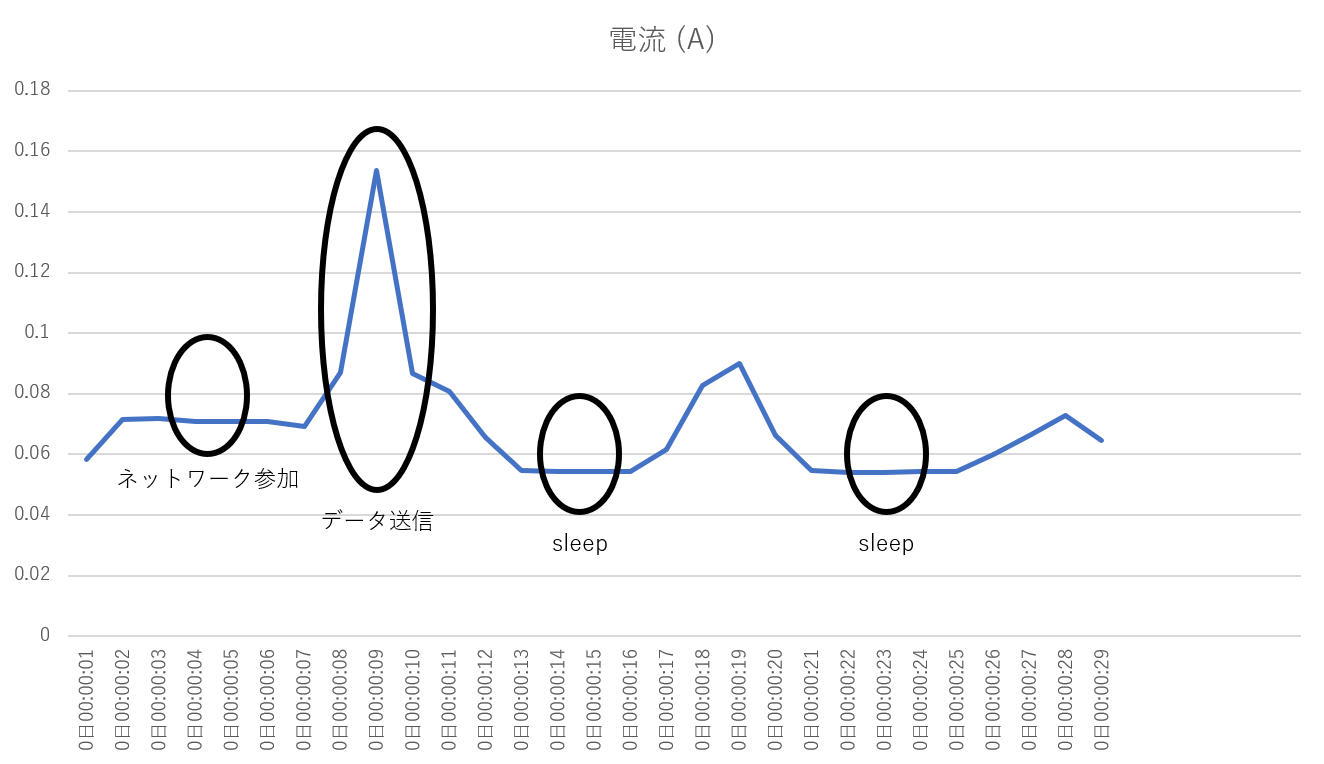
\includegraphics[width=15cm]{figures/LoRaWAN_消費電力実験.png}
    \caption{消費電力測定における各イベント(縦軸:消費電流,横軸:時間(s))}
    \label{fig:result_power_consumtion}
    \end{center}
\end{figure}

\begin{table}[]
    \caption{イベントごとの消費電力}\label{fig:LoRaWAN_PowerConsumption}
    \centering
    \begin{tabular}{|c|l|l|l|}
    \hline
    \textbf{イベント}     & \multicolumn{1}{c|}{\textbf{時間 (second)}} & \multicolumn{1}{c|}{\textbf{電流 (mA)}} & \multicolumn{1}{c|}{\textbf{消費電力 (mW)}} \\ \hline
    起動→ネットワーク参加       & 7                                         & 20                                    & 120                                     \\ \hline
    起動→ネットワーク参加→データ送信 & 11                                        & 21                                    & 105                                     \\ \hline
    スリープ              & なし                                        & 3                                     & 15                                      \\ \hline
    データ送信             & 4                                         & 29                                    & 145                                     \\ \hline
    \end{tabular}
\end{table}

\begin{table}[]
    \caption{その他パラメータ}\label{fig:LoRaWAN_Parameter}
    \centering
    \begin{tabular}{|c|c|}
    \hline
    \textbf{パラメータ} & \textbf{値} \\ \hline
    パケット到達率        & 90\%       \\ \hline
    RSSi           & -102       \\ \hline
    SNR            & -10        \\ \hline
    \end{tabular}
\end{table}
% % --- 研究課題 ---
% \chapter{実測に基づくグループ化アルゴリズムの適応点の評価}

\section{実験目的}
% 何を評価するために何を測って,どうなるとOKか,まで書いてください.
前項5.1.3(グループ化アルゴリズムの適応点の検討)で述べたように,グループ化の適応点を明らかにするため,LoRaWANにおける消費電力の実測を行う.適応点の評価については,前述したLoRaWANの既存方式と提案手法における関係式5.3に,実測した値を代入することで判断する.

\section{実験方法}
提案システムにおける各シーケンスにおいて消費電力を求めるため,起動からネットワーク参加,起動からネットワーク参加・初回送信,定常時の送信,スリープとイベントごと消費電力を計測する必要がある.実験では,市販のArduino互換LoRaWANモジュール及び消費電力計を用いて,消費電力を計測した.実験環境は,下記の表に示す.実験機材は,LoRaWANの送信機に,シングルボードコンピューターであるArduino Uno R3(表\ref{fig:Arduino_Spec}参照),LoRaWAN Shield for Arduino\cite{lorashield}(表\ref{fig:LoRaWAN_Spec}参照),受信機にLoRaWAN Gateway\cite{loragateway}(表\ref{fig:LoRaWAN_Gateway_Spec}),消費電力測定にマルチメータ\cite{kotomi}(表\ref{fig:Kotomi_Spec}参照)を用いた.LoRaWANは長距離伝送がユースケースであるため,LoRaWANのノードとGWノードを,高低差があり,約3.5kmの距離がある公立はこだて未来大学と自宅間に配置した.また計測結果を保存できる容量に限りがあるため,3試行を1セットとした.LoRaWANの設定内容を述べる.前述したLoRaWANのADR機能を適応し,スリープ時間は4秒とした.30秒間の計測を4セット12試行した.パケット到達率を算出するため,データ受信を確認する必要がある.本実測で利用したLoRaWANモジュールのプロバイダーは,MQTT ブローカーが提供しているため,MQTT クライアント\cite{mqtttool}を用いてデータを取得した.下記(図\ref{fig:experiment}参照)は,実験の様子である.

\begin{table}[]
    \caption{ARDUINO UNO REV3}\label{fig:Arduino_Spec}
    \centering
    \begin{tabular}{|c|c|}
    \hline
    動作電圧     & 5V   \\ \hline
    DC電流     & 50mA \\ \hline
    フラッシュメモリ & 32KB \\ \hline
    SRAM     & 2KB  \\ \hline
    EEPROM   & 1KB  \\ \hline
    \end{tabular}
\end{table}

\begin{table}[]
    \caption{LoRaWAN Shield for Arduino}\label{fig:LoRaWAN_Spec}
    \centering
    \begin{tabular}{|c|c|}
    \hline
    電源電圧 & DC2.2 $\sim$3.6V      \\ \hline
    周波数  & 920.6MHz $\sim$928MHz \\ \hline
    動作温度 & 0°C $\sim$40 °C       \\ \hline
    サイズ  & 68mm×53mm × 22.8mm    \\ \hline
    無線規格 & LoRaWAN 1.0.2         \\ \hline
    \end{tabular}
\end{table}

\begin{table}[]
    \caption{Kotomi Premium}\label{fig:Kotomi_Spec}
    \centering
    \begin{tabular}{|l|l|}
    \hline
    サイズ    & 77 x 35 x 13mm \\ \hline
    ディスプレイ & 1.44インチ        \\ \hline
    電圧精度   & 0.0001V        \\ \hline
    電流制度   & 0.0001A        \\ \hline
    電圧範囲   & 3.7~25V        \\ \hline
    電流範囲   & 0~5A           \\ \hline
    \end{tabular}
\end{table}

\begin{table}[]
    \caption{LoRaWAN Gateway}\label{fig:LoRaWAN_Gateway_Spec}
    \centering
    \begin{tabular}{|c|c|}
    \hline
    モデル名         & SW-GW01                       \\ \hline
    チャンネル数       & 最大8ch                         \\ \hline
    Wireless LAN & 802.11 b/g/n 2.4G             \\ \hline
    送信出力         & 20mW (最大13 dBm)               \\ \hline
    受信感度         & Down to -142 dBm              \\ \hline
    動作温度         & -10ºC $\sim$55ºC              \\ \hline
    電源電圧         & DC 5V / 2A(ミニUSBポート経由)        \\ \hline
    インターフェース     & Ethernet x 1ポート, 3/4G USBドングル \\ \hline
    サイズ          & L:116 x W:91 x H:27 mm        \\ \hline
    重量           & 160g                          \\ \hline
    \end{tabular}
\end{table}

\begin{table}[]
    \caption{実測に用いた電源}\label{fig:LoRaWAN_Battery}
    \centering
    \begin{tabular}{|c|c|}
    \hline
    サイズ     & 72 x 70 x 31 (mm) \\ \hline
    重量      & 189g              \\ \hline
    バッテリー容量 & 5000mAh           \\ \hline
    入力      & 5V=2A             \\ \hline
    出力      & 5V=3A             \\ \hline
    \end{tabular}
\end{table}

\begin{figure}[]
    \begin{center}
    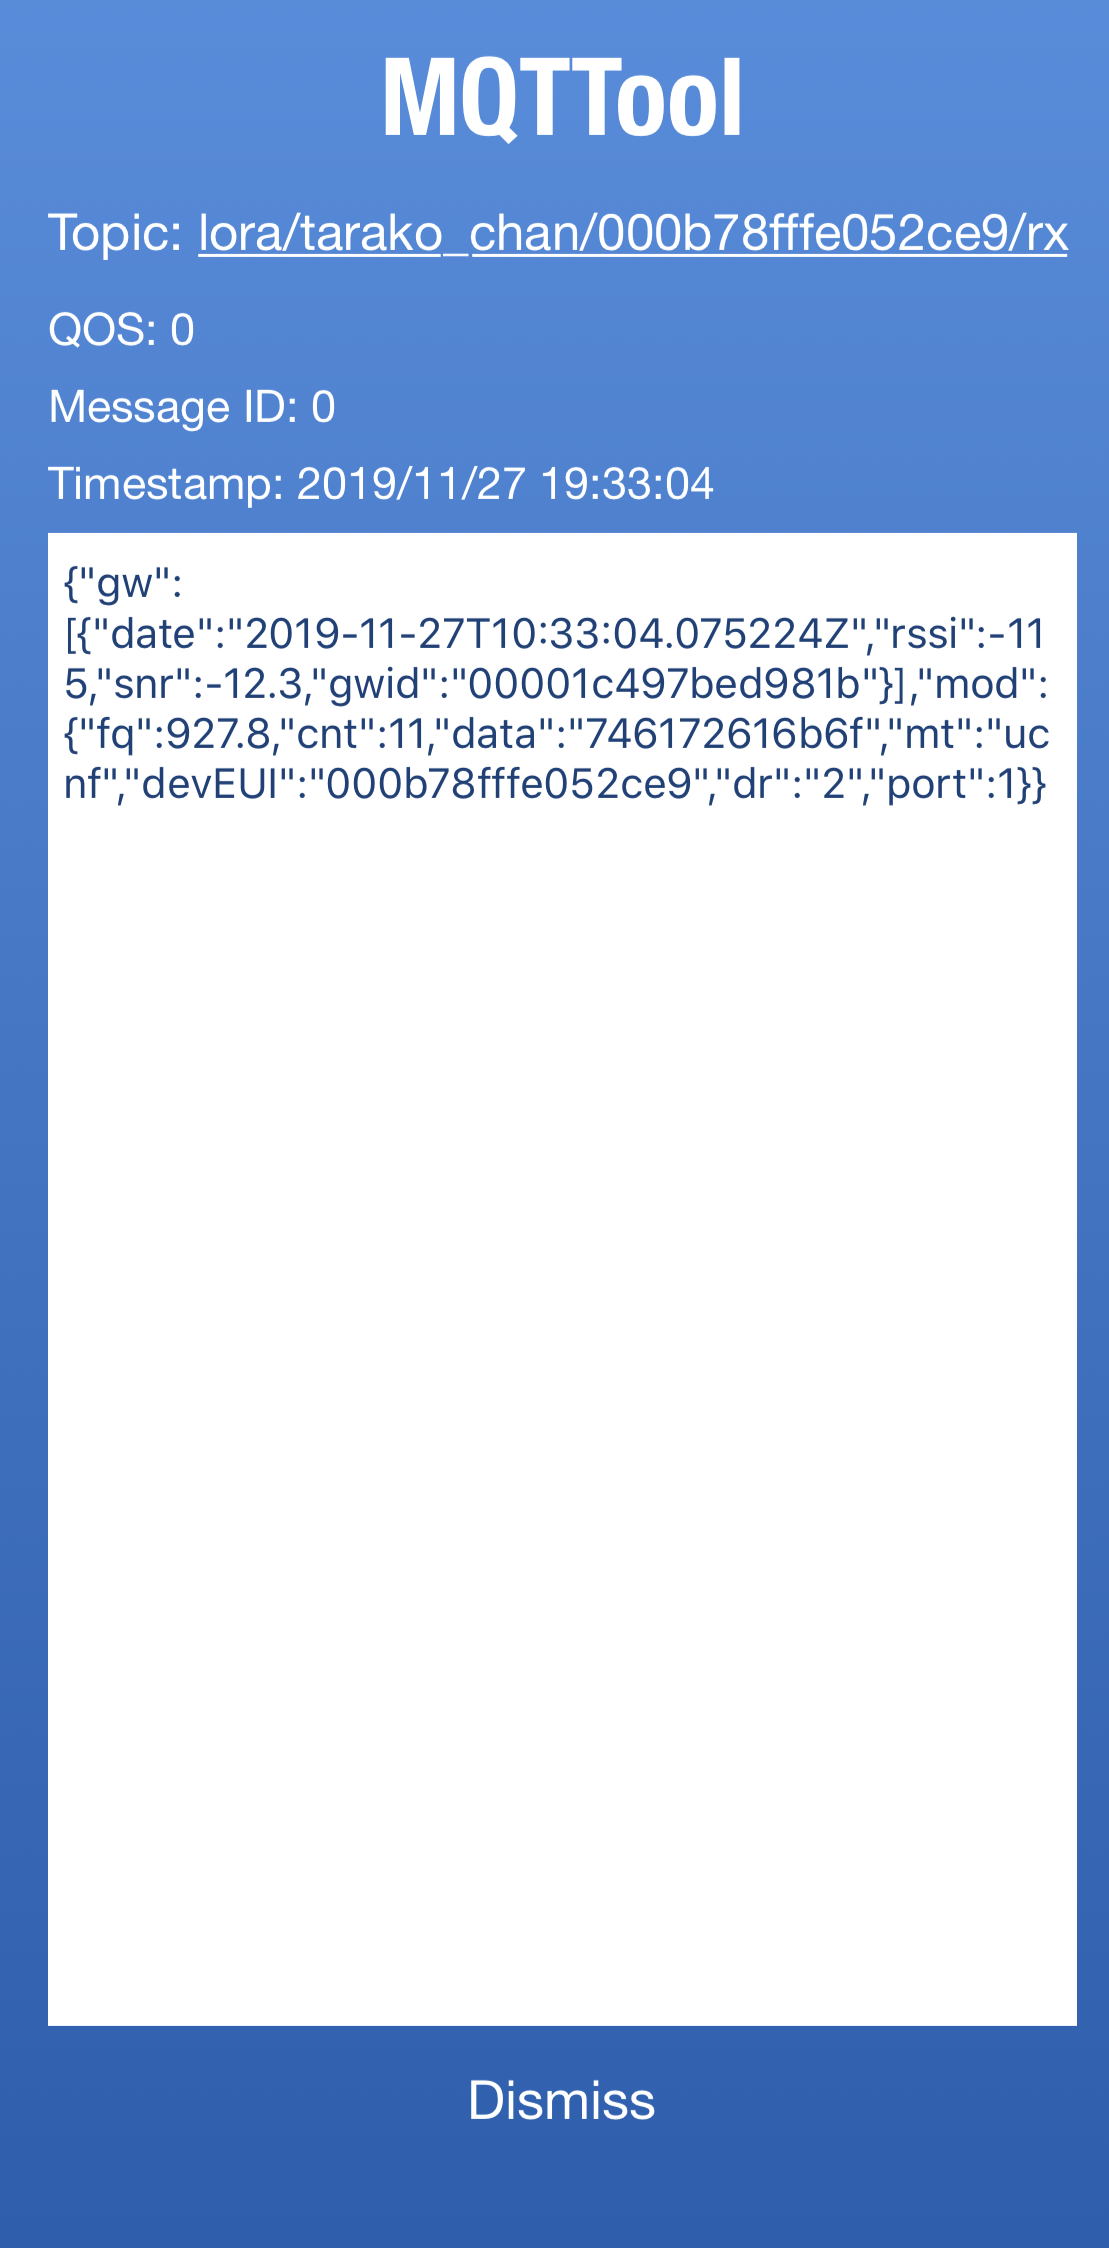
\includegraphics[width=5cm]{figures/mqtt.PNG}
    \caption{MQTT Client}
    \label{fig:mqtt}
    \end{center}
\end{figure}

\begin{figure}[]
    \begin{center}
    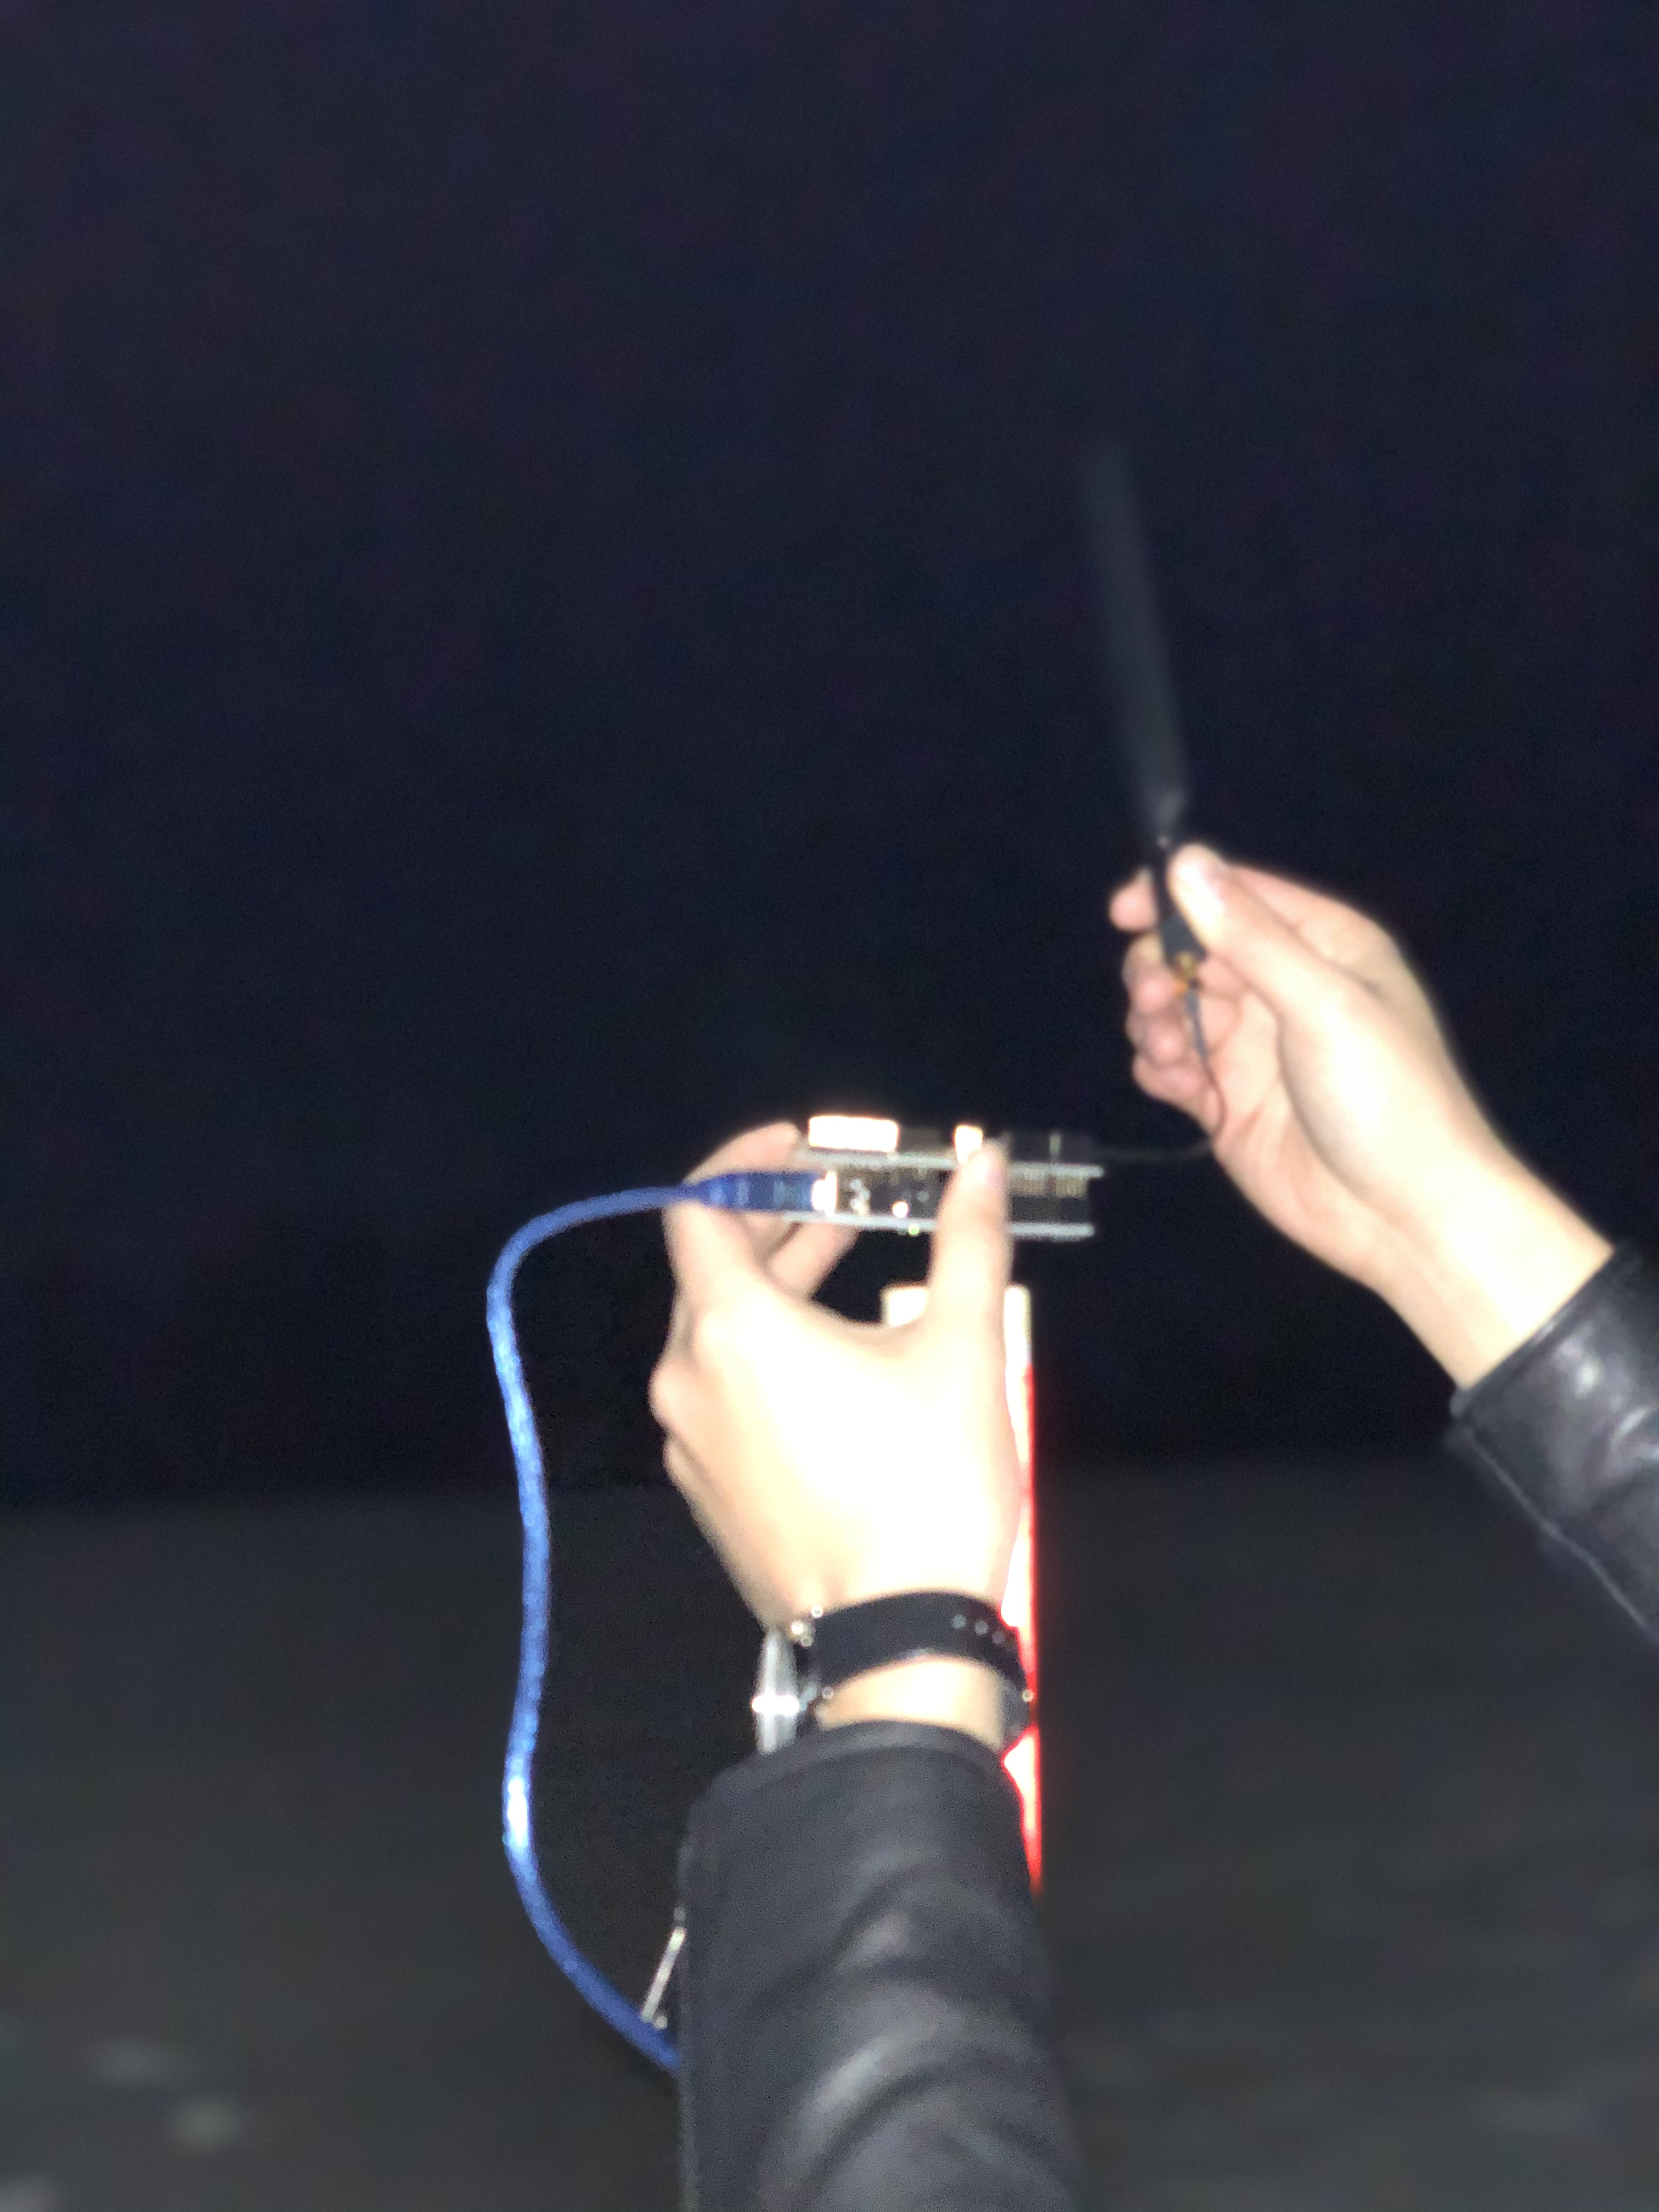
\includegraphics[width=5cm]{figures/experiment.jpg}
    \caption{実測実験の様子}
    \label{fig:experiment}
    \end{center}
\end{figure}

% ----
\section{実験結果}
LoRaWAN (DR2)でのイベントごとの消費電力実測結果を下記(表\ref{fig:result_power_consumtion}参照)(表\ref{fig:LoRaWAN_PowerConsumption}参照)に示す.また,LoRaWAN (DR2)でのその他値を下記(表\ref{fig:LoRaWAN_Parameter}参照)に示す.パケット到達率は,LoRaWANの送信回数に対してMQTTブローカーで受信したデータ数をもとに算出した.RSSiは,LoRaWANのGWノードが収集しMQTTブローカーに送信するため,その値を参考とした.SNRも同様である.

\begin{figure}[]
    \begin{center}
    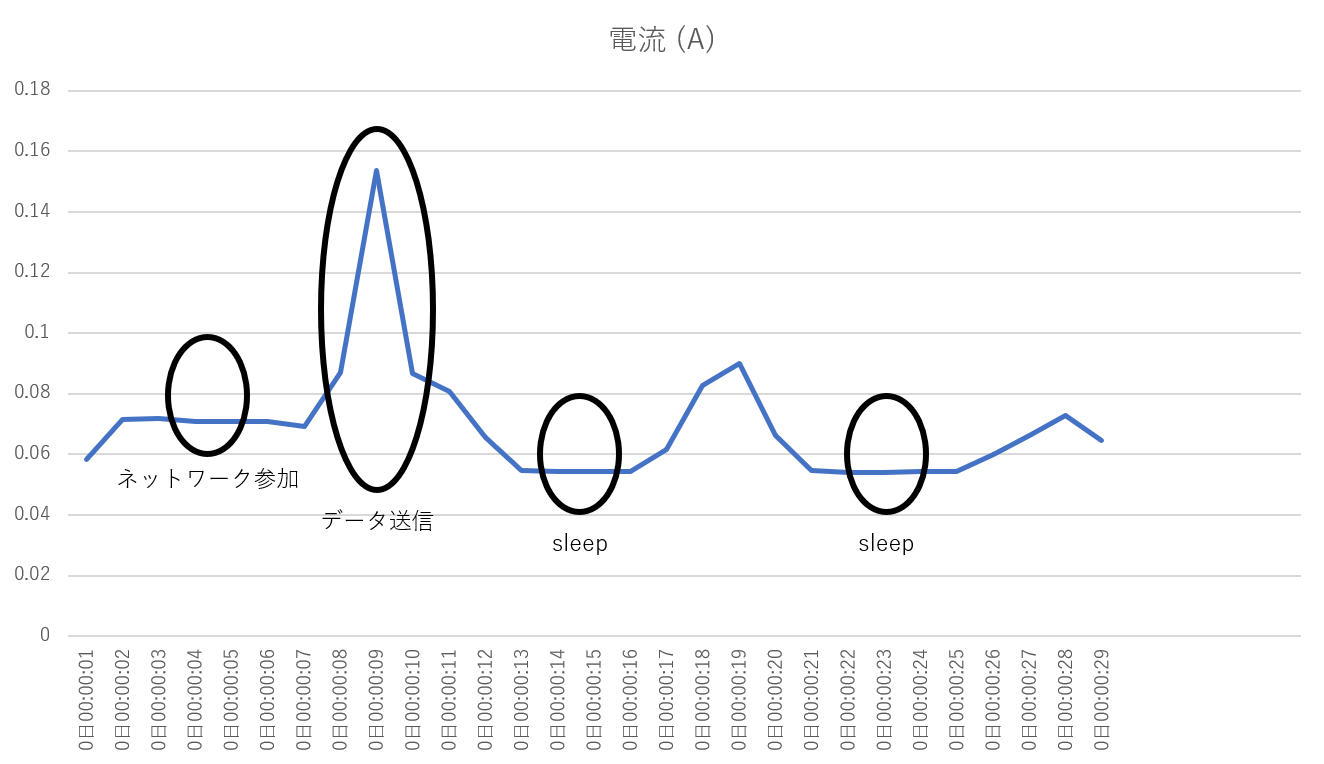
\includegraphics[width=15cm]{figures/LoRaWAN_消費電力実験.png}
    \caption{消費電力測定における各イベント(縦軸:消費電流,横軸:時間(s))}
    \label{fig:result_power_consumtion}
    \end{center}
\end{figure}

\begin{table}[]
    \caption{イベントごとの消費電力}\label{fig:LoRaWAN_PowerConsumption}
    \centering
    \begin{tabular}{|c|l|l|l|}
    \hline
    \textbf{イベント}     & \multicolumn{1}{c|}{\textbf{時間 (second)}} & \multicolumn{1}{c|}{\textbf{電流 (mA)}} & \multicolumn{1}{c|}{\textbf{消費電力 (mW)}} \\ \hline
    起動→ネットワーク参加       & 7                                         & 20                                    & 120                                     \\ \hline
    起動→ネットワーク参加→データ送信 & 11                                        & 21                                    & 105                                     \\ \hline
    スリープ              & なし                                        & 3                                     & 15                                      \\ \hline
    データ送信             & 4                                         & 29                                    & 145                                     \\ \hline
    \end{tabular}
\end{table}

\begin{table}[]
    \caption{その他パラメータ}\label{fig:LoRaWAN_Parameter}
    \centering
    \begin{tabular}{|c|c|}
    \hline
    \textbf{パラメータ} & \textbf{値} \\ \hline
    パケット到達率        & 90\%       \\ \hline
    RSSi           & -102       \\ \hline
    SNR            & -10        \\ \hline
    \end{tabular}
\end{table}
% % --- 提案手法 ---
% \chapter{実測に基づくグループ化アルゴリズムの適応点の評価}

\section{実験目的}
% 何を評価するために何を測って,どうなるとOKか,まで書いてください.
前項5.1.3(グループ化アルゴリズムの適応点の検討)で述べたように,グループ化の適応点を明らかにするため,LoRaWANにおける消費電力の実測を行う.適応点の評価については,前述したLoRaWANの既存方式と提案手法における関係式5.3に,実測した値を代入することで判断する.

\section{実験方法}
提案システムにおける各シーケンスにおいて消費電力を求めるため,起動からネットワーク参加,起動からネットワーク参加・初回送信,定常時の送信,スリープとイベントごと消費電力を計測する必要がある.実験では,市販のArduino互換LoRaWANモジュール及び消費電力計を用いて,消費電力を計測した.実験環境は,下記の表に示す.実験機材は,LoRaWANの送信機に,シングルボードコンピューターであるArduino Uno R3(表\ref{fig:Arduino_Spec}参照),LoRaWAN Shield for Arduino\cite{lorashield}(表\ref{fig:LoRaWAN_Spec}参照),受信機にLoRaWAN Gateway\cite{loragateway}(表\ref{fig:LoRaWAN_Gateway_Spec}),消費電力測定にマルチメータ\cite{kotomi}(表\ref{fig:Kotomi_Spec}参照)を用いた.LoRaWANは長距離伝送がユースケースであるため,LoRaWANのノードとGWノードを,高低差があり,約3.5kmの距離がある公立はこだて未来大学と自宅間に配置した.また計測結果を保存できる容量に限りがあるため,3試行を1セットとした.LoRaWANの設定内容を述べる.前述したLoRaWANのADR機能を適応し,スリープ時間は4秒とした.30秒間の計測を4セット12試行した.パケット到達率を算出するため,データ受信を確認する必要がある.本実測で利用したLoRaWANモジュールのプロバイダーは,MQTT ブローカーが提供しているため,MQTT クライアント\cite{mqtttool}を用いてデータを取得した.下記(図\ref{fig:experiment}参照)は,実験の様子である.

\begin{table}[]
    \caption{ARDUINO UNO REV3}\label{fig:Arduino_Spec}
    \centering
    \begin{tabular}{|c|c|}
    \hline
    動作電圧     & 5V   \\ \hline
    DC電流     & 50mA \\ \hline
    フラッシュメモリ & 32KB \\ \hline
    SRAM     & 2KB  \\ \hline
    EEPROM   & 1KB  \\ \hline
    \end{tabular}
\end{table}

\begin{table}[]
    \caption{LoRaWAN Shield for Arduino}\label{fig:LoRaWAN_Spec}
    \centering
    \begin{tabular}{|c|c|}
    \hline
    電源電圧 & DC2.2 $\sim$3.6V      \\ \hline
    周波数  & 920.6MHz $\sim$928MHz \\ \hline
    動作温度 & 0°C $\sim$40 °C       \\ \hline
    サイズ  & 68mm×53mm × 22.8mm    \\ \hline
    無線規格 & LoRaWAN 1.0.2         \\ \hline
    \end{tabular}
\end{table}

\begin{table}[]
    \caption{Kotomi Premium}\label{fig:Kotomi_Spec}
    \centering
    \begin{tabular}{|l|l|}
    \hline
    サイズ    & 77 x 35 x 13mm \\ \hline
    ディスプレイ & 1.44インチ        \\ \hline
    電圧精度   & 0.0001V        \\ \hline
    電流制度   & 0.0001A        \\ \hline
    電圧範囲   & 3.7~25V        \\ \hline
    電流範囲   & 0~5A           \\ \hline
    \end{tabular}
\end{table}

\begin{table}[]
    \caption{LoRaWAN Gateway}\label{fig:LoRaWAN_Gateway_Spec}
    \centering
    \begin{tabular}{|c|c|}
    \hline
    モデル名         & SW-GW01                       \\ \hline
    チャンネル数       & 最大8ch                         \\ \hline
    Wireless LAN & 802.11 b/g/n 2.4G             \\ \hline
    送信出力         & 20mW (最大13 dBm)               \\ \hline
    受信感度         & Down to -142 dBm              \\ \hline
    動作温度         & -10ºC $\sim$55ºC              \\ \hline
    電源電圧         & DC 5V / 2A(ミニUSBポート経由)        \\ \hline
    インターフェース     & Ethernet x 1ポート, 3/4G USBドングル \\ \hline
    サイズ          & L:116 x W:91 x H:27 mm        \\ \hline
    重量           & 160g                          \\ \hline
    \end{tabular}
\end{table}

\begin{table}[]
    \caption{実測に用いた電源}\label{fig:LoRaWAN_Battery}
    \centering
    \begin{tabular}{|c|c|}
    \hline
    サイズ     & 72 x 70 x 31 (mm) \\ \hline
    重量      & 189g              \\ \hline
    バッテリー容量 & 5000mAh           \\ \hline
    入力      & 5V=2A             \\ \hline
    出力      & 5V=3A             \\ \hline
    \end{tabular}
\end{table}

\begin{figure}[]
    \begin{center}
    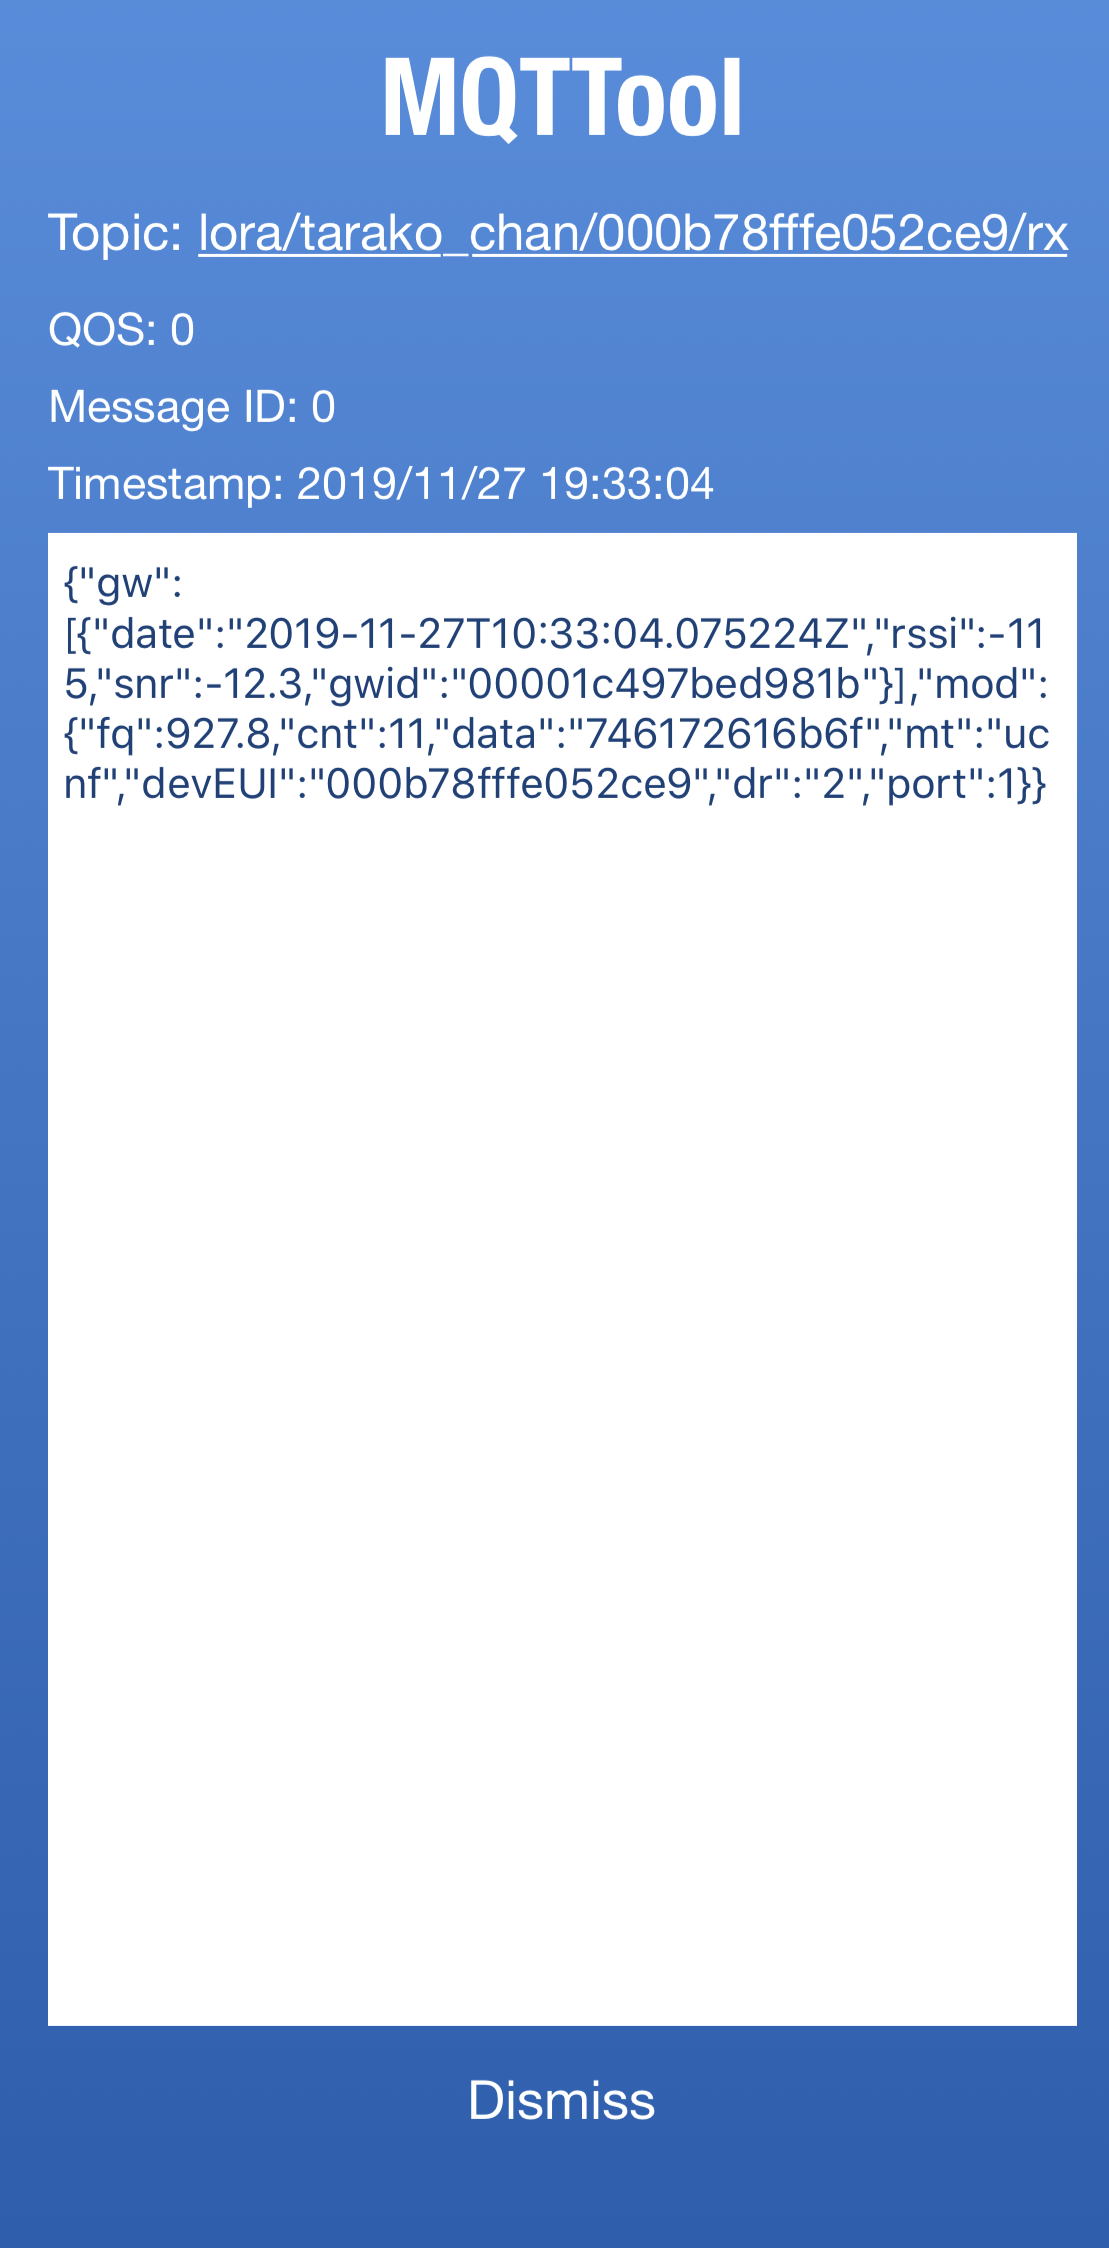
\includegraphics[width=5cm]{figures/mqtt.PNG}
    \caption{MQTT Client}
    \label{fig:mqtt}
    \end{center}
\end{figure}

\begin{figure}[]
    \begin{center}
    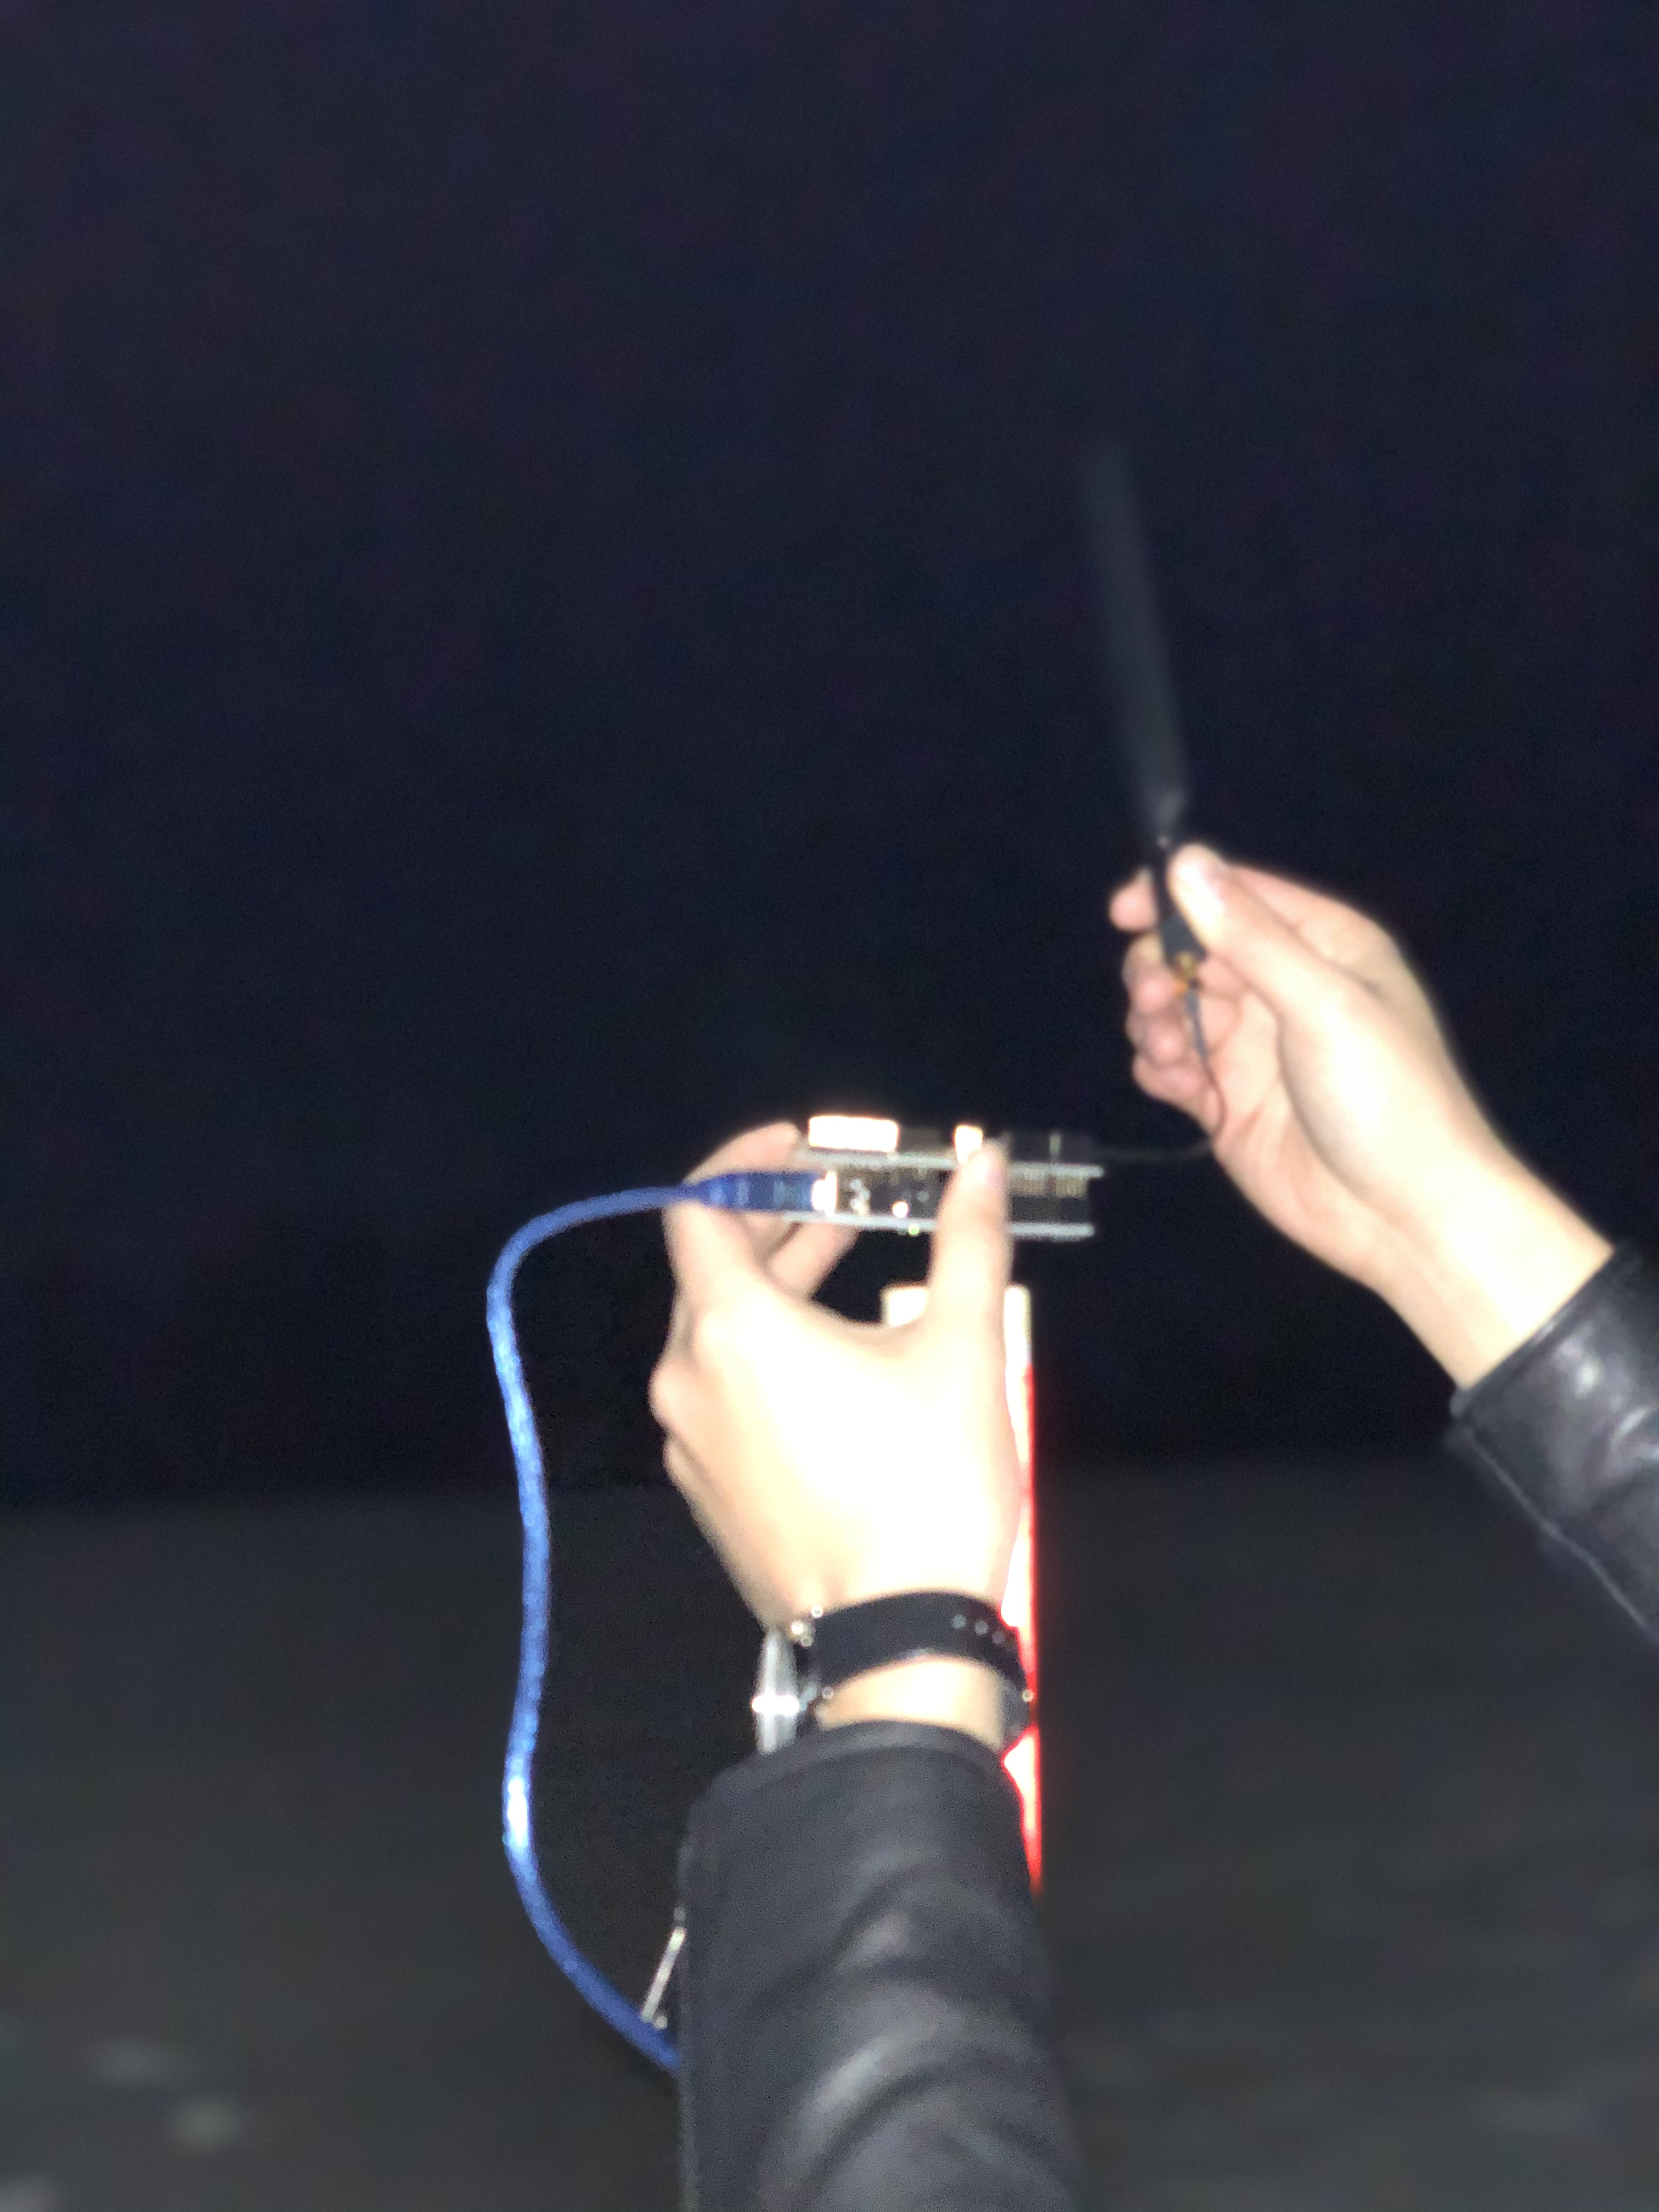
\includegraphics[width=5cm]{figures/experiment.jpg}
    \caption{実測実験の様子}
    \label{fig:experiment}
    \end{center}
\end{figure}

% ----
\section{実験結果}
LoRaWAN (DR2)でのイベントごとの消費電力実測結果を下記(表\ref{fig:result_power_consumtion}参照)(表\ref{fig:LoRaWAN_PowerConsumption}参照)に示す.また,LoRaWAN (DR2)でのその他値を下記(表\ref{fig:LoRaWAN_Parameter}参照)に示す.パケット到達率は,LoRaWANの送信回数に対してMQTTブローカーで受信したデータ数をもとに算出した.RSSiは,LoRaWANのGWノードが収集しMQTTブローカーに送信するため,その値を参考とした.SNRも同様である.

\begin{figure}[]
    \begin{center}
    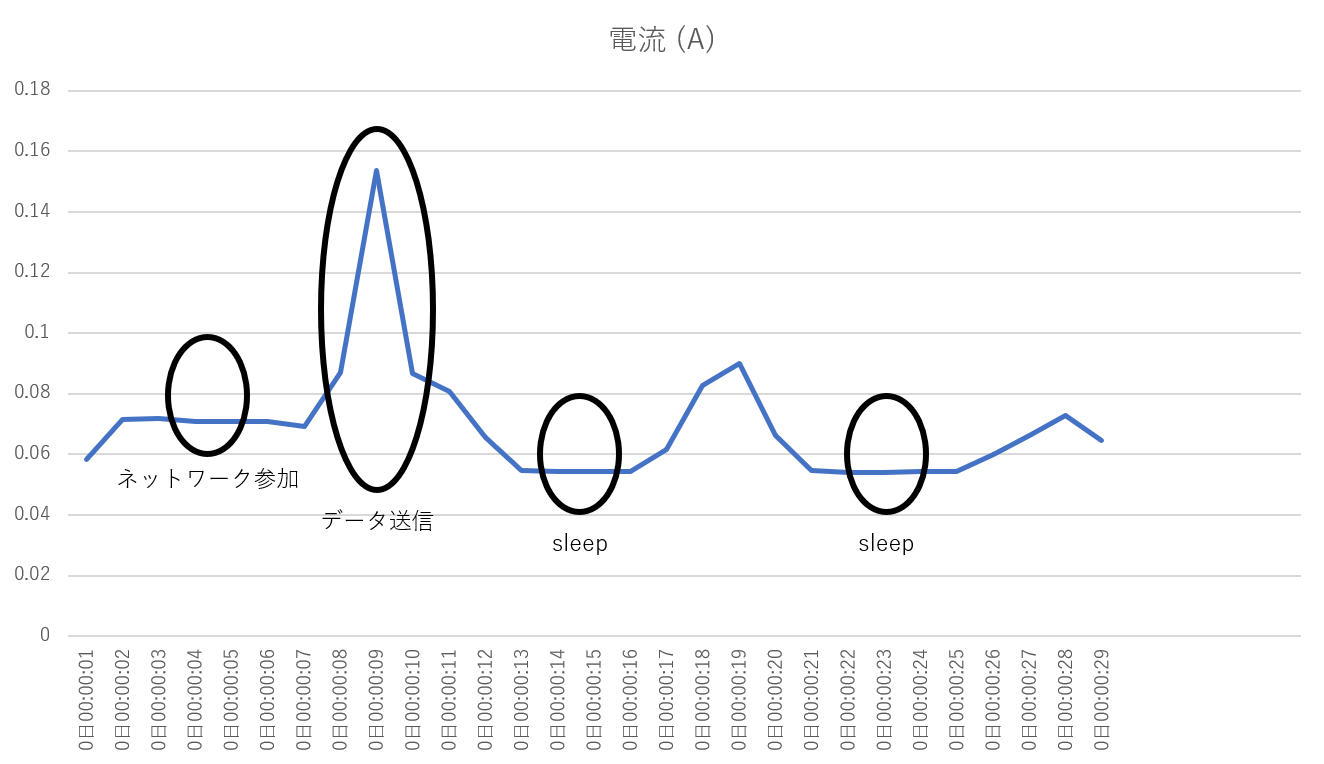
\includegraphics[width=15cm]{figures/LoRaWAN_消費電力実験.png}
    \caption{消費電力測定における各イベント(縦軸:消費電流,横軸:時間(s))}
    \label{fig:result_power_consumtion}
    \end{center}
\end{figure}

\begin{table}[]
    \caption{イベントごとの消費電力}\label{fig:LoRaWAN_PowerConsumption}
    \centering
    \begin{tabular}{|c|l|l|l|}
    \hline
    \textbf{イベント}     & \multicolumn{1}{c|}{\textbf{時間 (second)}} & \multicolumn{1}{c|}{\textbf{電流 (mA)}} & \multicolumn{1}{c|}{\textbf{消費電力 (mW)}} \\ \hline
    起動→ネットワーク参加       & 7                                         & 20                                    & 120                                     \\ \hline
    起動→ネットワーク参加→データ送信 & 11                                        & 21                                    & 105                                     \\ \hline
    スリープ              & なし                                        & 3                                     & 15                                      \\ \hline
    データ送信             & 4                                         & 29                                    & 145                                     \\ \hline
    \end{tabular}
\end{table}

\begin{table}[]
    \caption{その他パラメータ}\label{fig:LoRaWAN_Parameter}
    \centering
    \begin{tabular}{|c|c|}
    \hline
    \textbf{パラメータ} & \textbf{値} \\ \hline
    パケット到達率        & 90\%       \\ \hline
    RSSi           & -102       \\ \hline
    SNR            & -10        \\ \hline
    \end{tabular}
\end{table}
% % --- 実験と評価 ---
% \chapter{実測に基づくグループ化アルゴリズムの適応点の評価}

\section{実験目的}
% 何を評価するために何を測って,どうなるとOKか,まで書いてください.
前項5.1.3(グループ化アルゴリズムの適応点の検討)で述べたように,グループ化の適応点を明らかにするため,LoRaWANにおける消費電力の実測を行う.適応点の評価については,前述したLoRaWANの既存方式と提案手法における関係式5.3に,実測した値を代入することで判断する.

\section{実験方法}
提案システムにおける各シーケンスにおいて消費電力を求めるため,起動からネットワーク参加,起動からネットワーク参加・初回送信,定常時の送信,スリープとイベントごと消費電力を計測する必要がある.実験では,市販のArduino互換LoRaWANモジュール及び消費電力計を用いて,消費電力を計測した.実験環境は,下記の表に示す.実験機材は,LoRaWANの送信機に,シングルボードコンピューターであるArduino Uno R3(表\ref{fig:Arduino_Spec}参照),LoRaWAN Shield for Arduino\cite{lorashield}(表\ref{fig:LoRaWAN_Spec}参照),受信機にLoRaWAN Gateway\cite{loragateway}(表\ref{fig:LoRaWAN_Gateway_Spec}),消費電力測定にマルチメータ\cite{kotomi}(表\ref{fig:Kotomi_Spec}参照)を用いた.LoRaWANは長距離伝送がユースケースであるため,LoRaWANのノードとGWノードを,高低差があり,約3.5kmの距離がある公立はこだて未来大学と自宅間に配置した.また計測結果を保存できる容量に限りがあるため,3試行を1セットとした.LoRaWANの設定内容を述べる.前述したLoRaWANのADR機能を適応し,スリープ時間は4秒とした.30秒間の計測を4セット12試行した.パケット到達率を算出するため,データ受信を確認する必要がある.本実測で利用したLoRaWANモジュールのプロバイダーは,MQTT ブローカーが提供しているため,MQTT クライアント\cite{mqtttool}を用いてデータを取得した.下記(図\ref{fig:experiment}参照)は,実験の様子である.

\begin{table}[]
    \caption{ARDUINO UNO REV3}\label{fig:Arduino_Spec}
    \centering
    \begin{tabular}{|c|c|}
    \hline
    動作電圧     & 5V   \\ \hline
    DC電流     & 50mA \\ \hline
    フラッシュメモリ & 32KB \\ \hline
    SRAM     & 2KB  \\ \hline
    EEPROM   & 1KB  \\ \hline
    \end{tabular}
\end{table}

\begin{table}[]
    \caption{LoRaWAN Shield for Arduino}\label{fig:LoRaWAN_Spec}
    \centering
    \begin{tabular}{|c|c|}
    \hline
    電源電圧 & DC2.2 $\sim$3.6V      \\ \hline
    周波数  & 920.6MHz $\sim$928MHz \\ \hline
    動作温度 & 0°C $\sim$40 °C       \\ \hline
    サイズ  & 68mm×53mm × 22.8mm    \\ \hline
    無線規格 & LoRaWAN 1.0.2         \\ \hline
    \end{tabular}
\end{table}

\begin{table}[]
    \caption{Kotomi Premium}\label{fig:Kotomi_Spec}
    \centering
    \begin{tabular}{|l|l|}
    \hline
    サイズ    & 77 x 35 x 13mm \\ \hline
    ディスプレイ & 1.44インチ        \\ \hline
    電圧精度   & 0.0001V        \\ \hline
    電流制度   & 0.0001A        \\ \hline
    電圧範囲   & 3.7~25V        \\ \hline
    電流範囲   & 0~5A           \\ \hline
    \end{tabular}
\end{table}

\begin{table}[]
    \caption{LoRaWAN Gateway}\label{fig:LoRaWAN_Gateway_Spec}
    \centering
    \begin{tabular}{|c|c|}
    \hline
    モデル名         & SW-GW01                       \\ \hline
    チャンネル数       & 最大8ch                         \\ \hline
    Wireless LAN & 802.11 b/g/n 2.4G             \\ \hline
    送信出力         & 20mW (最大13 dBm)               \\ \hline
    受信感度         & Down to -142 dBm              \\ \hline
    動作温度         & -10ºC $\sim$55ºC              \\ \hline
    電源電圧         & DC 5V / 2A(ミニUSBポート経由)        \\ \hline
    インターフェース     & Ethernet x 1ポート, 3/4G USBドングル \\ \hline
    サイズ          & L:116 x W:91 x H:27 mm        \\ \hline
    重量           & 160g                          \\ \hline
    \end{tabular}
\end{table}

\begin{table}[]
    \caption{実測に用いた電源}\label{fig:LoRaWAN_Battery}
    \centering
    \begin{tabular}{|c|c|}
    \hline
    サイズ     & 72 x 70 x 31 (mm) \\ \hline
    重量      & 189g              \\ \hline
    バッテリー容量 & 5000mAh           \\ \hline
    入力      & 5V=2A             \\ \hline
    出力      & 5V=3A             \\ \hline
    \end{tabular}
\end{table}

\begin{figure}[]
    \begin{center}
    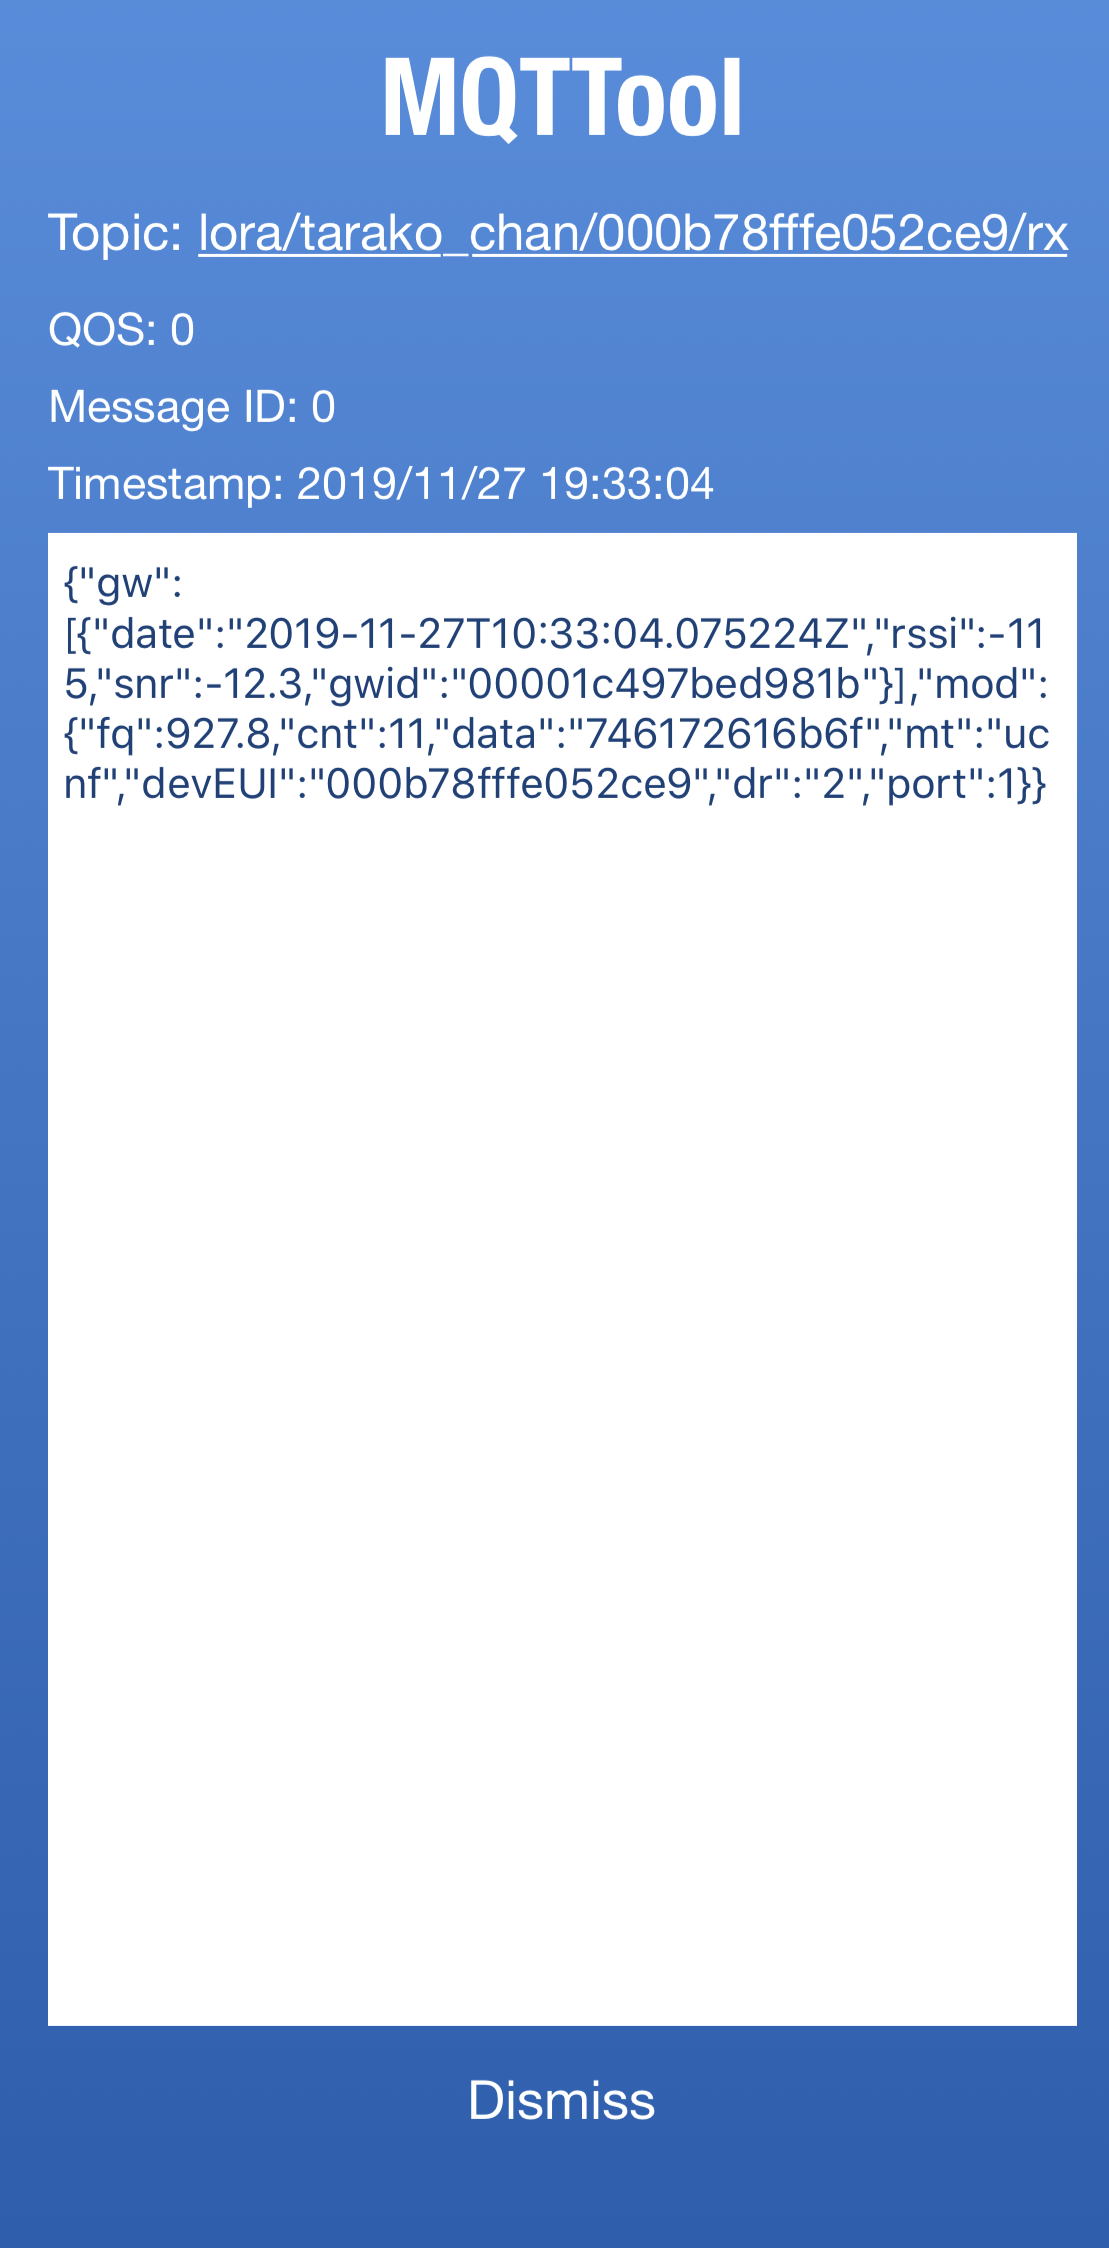
\includegraphics[width=5cm]{figures/mqtt.PNG}
    \caption{MQTT Client}
    \label{fig:mqtt}
    \end{center}
\end{figure}

\begin{figure}[]
    \begin{center}
    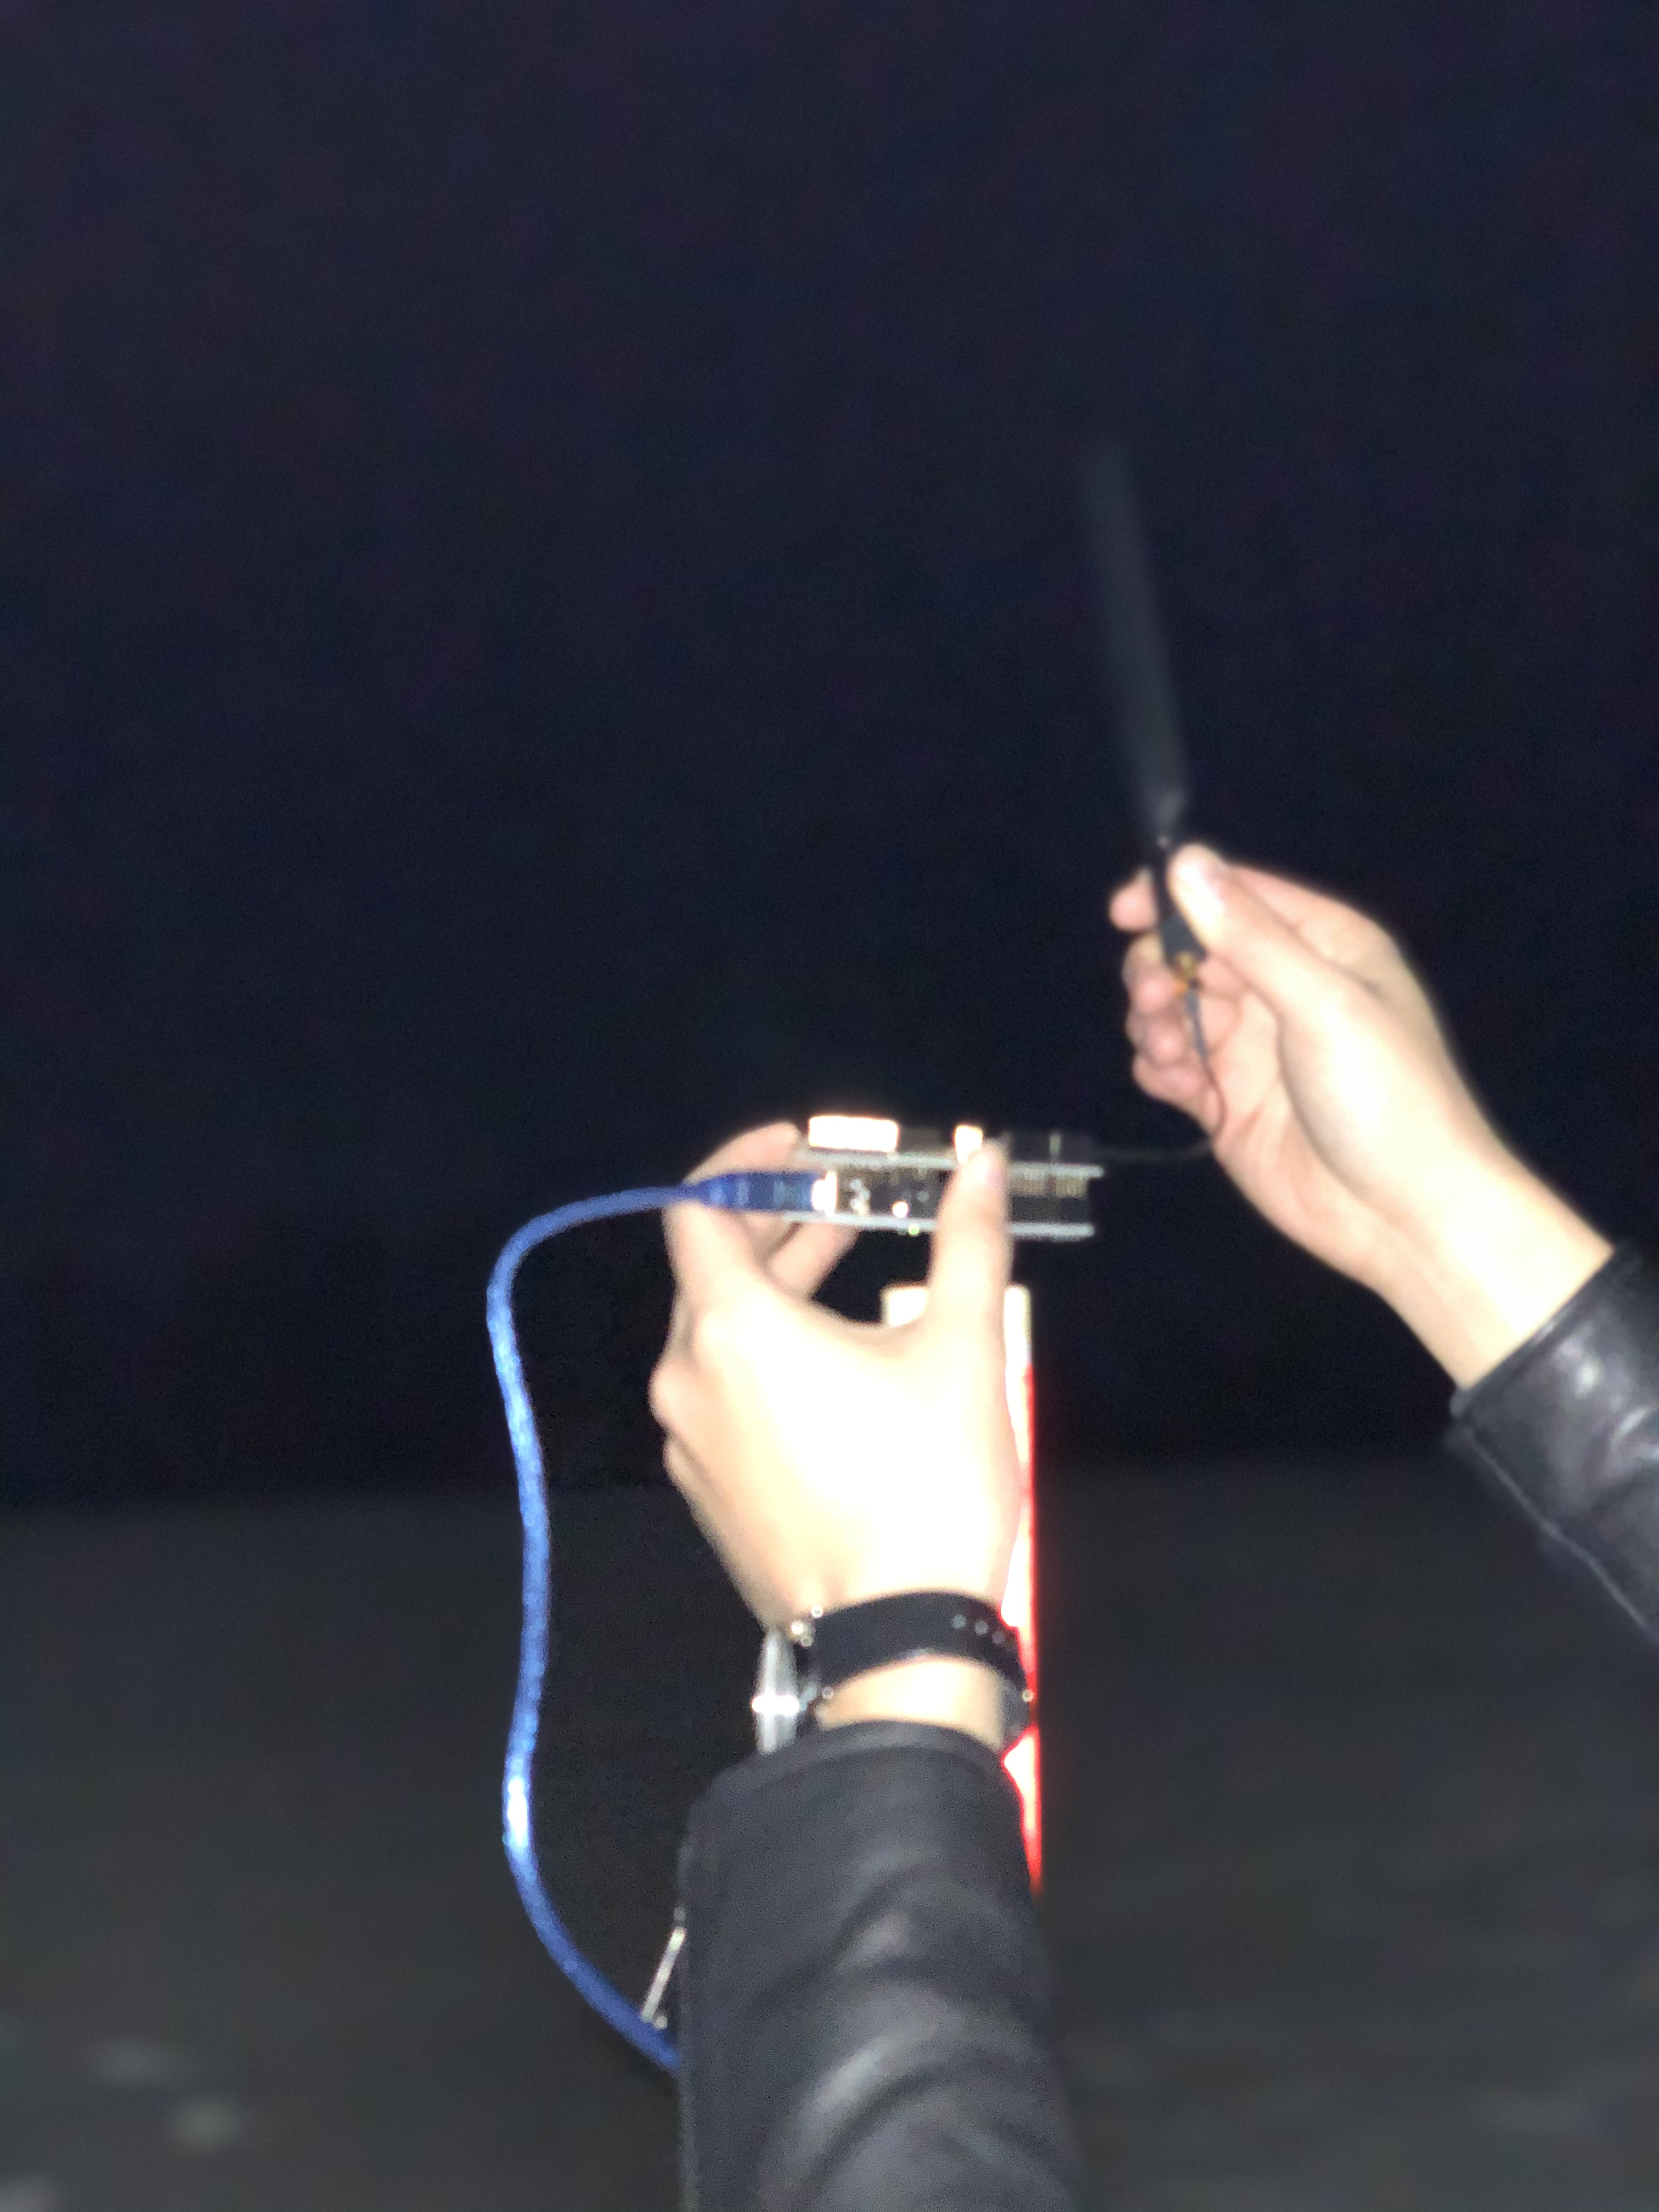
\includegraphics[width=5cm]{figures/experiment.jpg}
    \caption{実測実験の様子}
    \label{fig:experiment}
    \end{center}
\end{figure}

% ----
\section{実験結果}
LoRaWAN (DR2)でのイベントごとの消費電力実測結果を下記(表\ref{fig:result_power_consumtion}参照)(表\ref{fig:LoRaWAN_PowerConsumption}参照)に示す.また,LoRaWAN (DR2)でのその他値を下記(表\ref{fig:LoRaWAN_Parameter}参照)に示す.パケット到達率は,LoRaWANの送信回数に対してMQTTブローカーで受信したデータ数をもとに算出した.RSSiは,LoRaWANのGWノードが収集しMQTTブローカーに送信するため,その値を参考とした.SNRも同様である.

\begin{figure}[]
    \begin{center}
    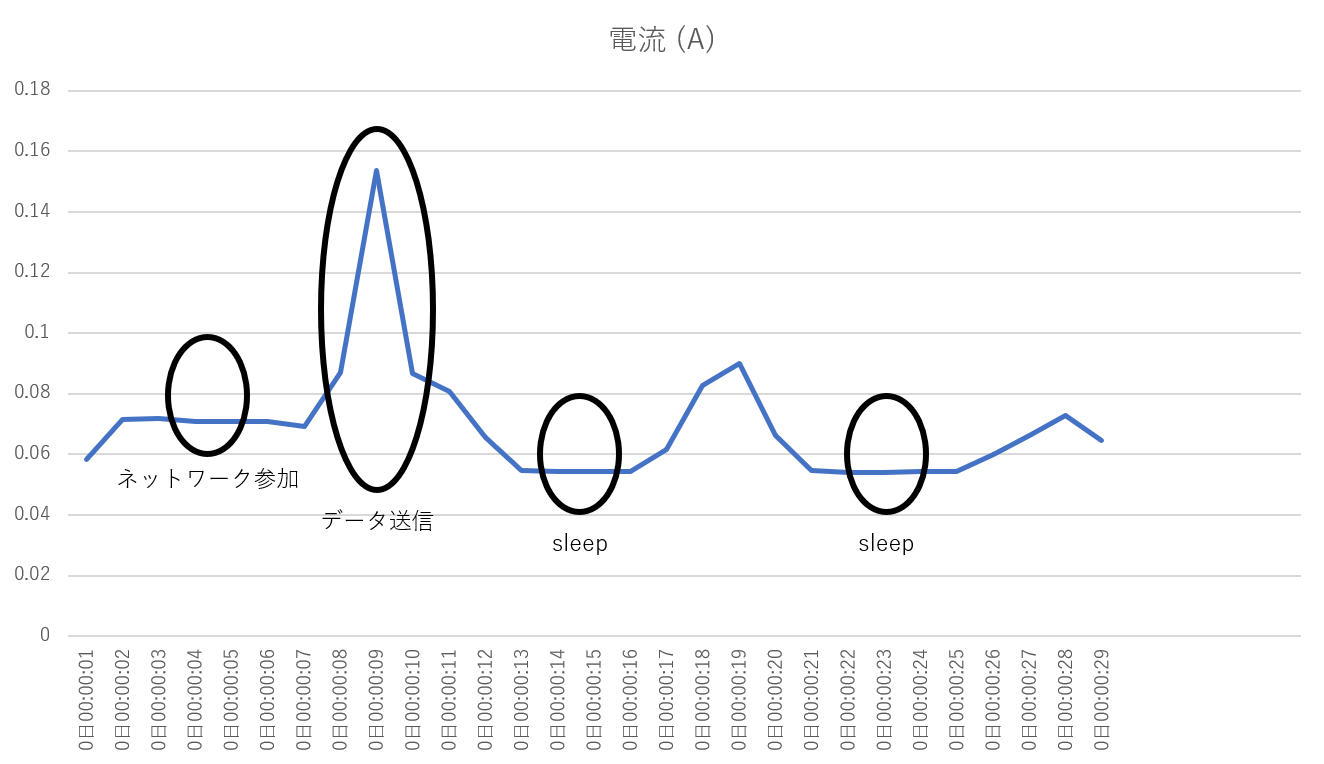
\includegraphics[width=15cm]{figures/LoRaWAN_消費電力実験.png}
    \caption{消費電力測定における各イベント(縦軸:消費電流,横軸:時間(s))}
    \label{fig:result_power_consumtion}
    \end{center}
\end{figure}

\begin{table}[]
    \caption{イベントごとの消費電力}\label{fig:LoRaWAN_PowerConsumption}
    \centering
    \begin{tabular}{|c|l|l|l|}
    \hline
    \textbf{イベント}     & \multicolumn{1}{c|}{\textbf{時間 (second)}} & \multicolumn{1}{c|}{\textbf{電流 (mA)}} & \multicolumn{1}{c|}{\textbf{消費電力 (mW)}} \\ \hline
    起動→ネットワーク参加       & 7                                         & 20                                    & 120                                     \\ \hline
    起動→ネットワーク参加→データ送信 & 11                                        & 21                                    & 105                                     \\ \hline
    スリープ              & なし                                        & 3                                     & 15                                      \\ \hline
    データ送信             & 4                                         & 29                                    & 145                                     \\ \hline
    \end{tabular}
\end{table}

\begin{table}[]
    \caption{その他パラメータ}\label{fig:LoRaWAN_Parameter}
    \centering
    \begin{tabular}{|c|c|}
    \hline
    \textbf{パラメータ} & \textbf{値} \\ \hline
    パケット到達率        & 90\%       \\ \hline
    RSSi           & -102       \\ \hline
    SNR            & -10        \\ \hline
    \end{tabular}
\end{table}
% % --- 考察 ---
% \chapter{実測に基づくグループ化アルゴリズムの適応点の評価}

\section{実験目的}
% 何を評価するために何を測って,どうなるとOKか,まで書いてください.
前項5.1.3(グループ化アルゴリズムの適応点の検討)で述べたように,グループ化の適応点を明らかにするため,LoRaWANにおける消費電力の実測を行う.適応点の評価については,前述したLoRaWANの既存方式と提案手法における関係式5.3に,実測した値を代入することで判断する.

\section{実験方法}
提案システムにおける各シーケンスにおいて消費電力を求めるため,起動からネットワーク参加,起動からネットワーク参加・初回送信,定常時の送信,スリープとイベントごと消費電力を計測する必要がある.実験では,市販のArduino互換LoRaWANモジュール及び消費電力計を用いて,消費電力を計測した.実験環境は,下記の表に示す.実験機材は,LoRaWANの送信機に,シングルボードコンピューターであるArduino Uno R3(表\ref{fig:Arduino_Spec}参照),LoRaWAN Shield for Arduino\cite{lorashield}(表\ref{fig:LoRaWAN_Spec}参照),受信機にLoRaWAN Gateway\cite{loragateway}(表\ref{fig:LoRaWAN_Gateway_Spec}),消費電力測定にマルチメータ\cite{kotomi}(表\ref{fig:Kotomi_Spec}参照)を用いた.LoRaWANは長距離伝送がユースケースであるため,LoRaWANのノードとGWノードを,高低差があり,約3.5kmの距離がある公立はこだて未来大学と自宅間に配置した.また計測結果を保存できる容量に限りがあるため,3試行を1セットとした.LoRaWANの設定内容を述べる.前述したLoRaWANのADR機能を適応し,スリープ時間は4秒とした.30秒間の計測を4セット12試行した.パケット到達率を算出するため,データ受信を確認する必要がある.本実測で利用したLoRaWANモジュールのプロバイダーは,MQTT ブローカーが提供しているため,MQTT クライアント\cite{mqtttool}を用いてデータを取得した.下記(図\ref{fig:experiment}参照)は,実験の様子である.

\begin{table}[]
    \caption{ARDUINO UNO REV3}\label{fig:Arduino_Spec}
    \centering
    \begin{tabular}{|c|c|}
    \hline
    動作電圧     & 5V   \\ \hline
    DC電流     & 50mA \\ \hline
    フラッシュメモリ & 32KB \\ \hline
    SRAM     & 2KB  \\ \hline
    EEPROM   & 1KB  \\ \hline
    \end{tabular}
\end{table}

\begin{table}[]
    \caption{LoRaWAN Shield for Arduino}\label{fig:LoRaWAN_Spec}
    \centering
    \begin{tabular}{|c|c|}
    \hline
    電源電圧 & DC2.2 $\sim$3.6V      \\ \hline
    周波数  & 920.6MHz $\sim$928MHz \\ \hline
    動作温度 & 0°C $\sim$40 °C       \\ \hline
    サイズ  & 68mm×53mm × 22.8mm    \\ \hline
    無線規格 & LoRaWAN 1.0.2         \\ \hline
    \end{tabular}
\end{table}

\begin{table}[]
    \caption{Kotomi Premium}\label{fig:Kotomi_Spec}
    \centering
    \begin{tabular}{|l|l|}
    \hline
    サイズ    & 77 x 35 x 13mm \\ \hline
    ディスプレイ & 1.44インチ        \\ \hline
    電圧精度   & 0.0001V        \\ \hline
    電流制度   & 0.0001A        \\ \hline
    電圧範囲   & 3.7~25V        \\ \hline
    電流範囲   & 0~5A           \\ \hline
    \end{tabular}
\end{table}

\begin{table}[]
    \caption{LoRaWAN Gateway}\label{fig:LoRaWAN_Gateway_Spec}
    \centering
    \begin{tabular}{|c|c|}
    \hline
    モデル名         & SW-GW01                       \\ \hline
    チャンネル数       & 最大8ch                         \\ \hline
    Wireless LAN & 802.11 b/g/n 2.4G             \\ \hline
    送信出力         & 20mW (最大13 dBm)               \\ \hline
    受信感度         & Down to -142 dBm              \\ \hline
    動作温度         & -10ºC $\sim$55ºC              \\ \hline
    電源電圧         & DC 5V / 2A(ミニUSBポート経由)        \\ \hline
    インターフェース     & Ethernet x 1ポート, 3/4G USBドングル \\ \hline
    サイズ          & L:116 x W:91 x H:27 mm        \\ \hline
    重量           & 160g                          \\ \hline
    \end{tabular}
\end{table}

\begin{table}[]
    \caption{実測に用いた電源}\label{fig:LoRaWAN_Battery}
    \centering
    \begin{tabular}{|c|c|}
    \hline
    サイズ     & 72 x 70 x 31 (mm) \\ \hline
    重量      & 189g              \\ \hline
    バッテリー容量 & 5000mAh           \\ \hline
    入力      & 5V=2A             \\ \hline
    出力      & 5V=3A             \\ \hline
    \end{tabular}
\end{table}

\begin{figure}[]
    \begin{center}
    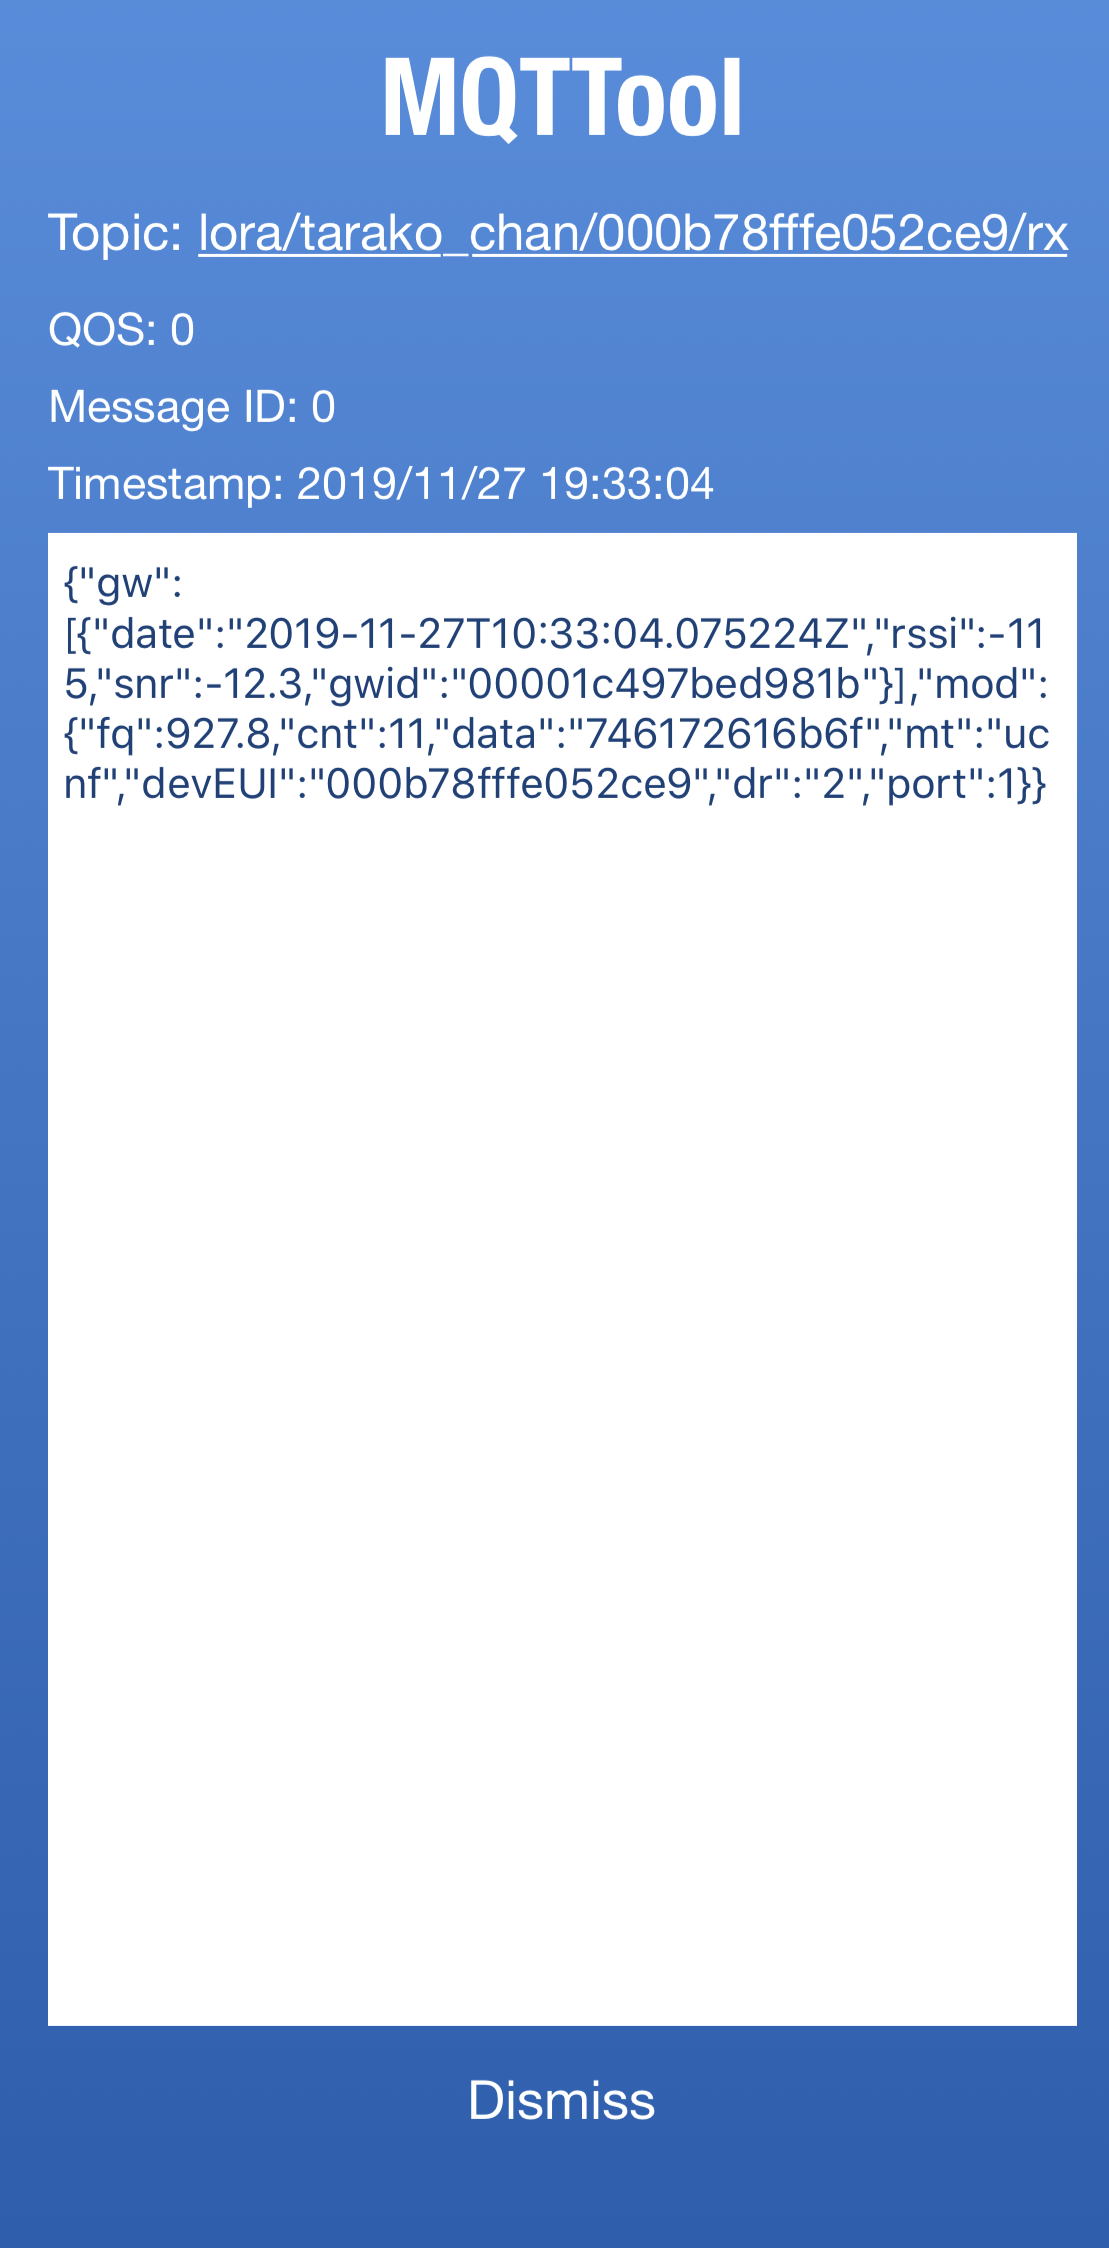
\includegraphics[width=5cm]{figures/mqtt.PNG}
    \caption{MQTT Client}
    \label{fig:mqtt}
    \end{center}
\end{figure}

\begin{figure}[]
    \begin{center}
    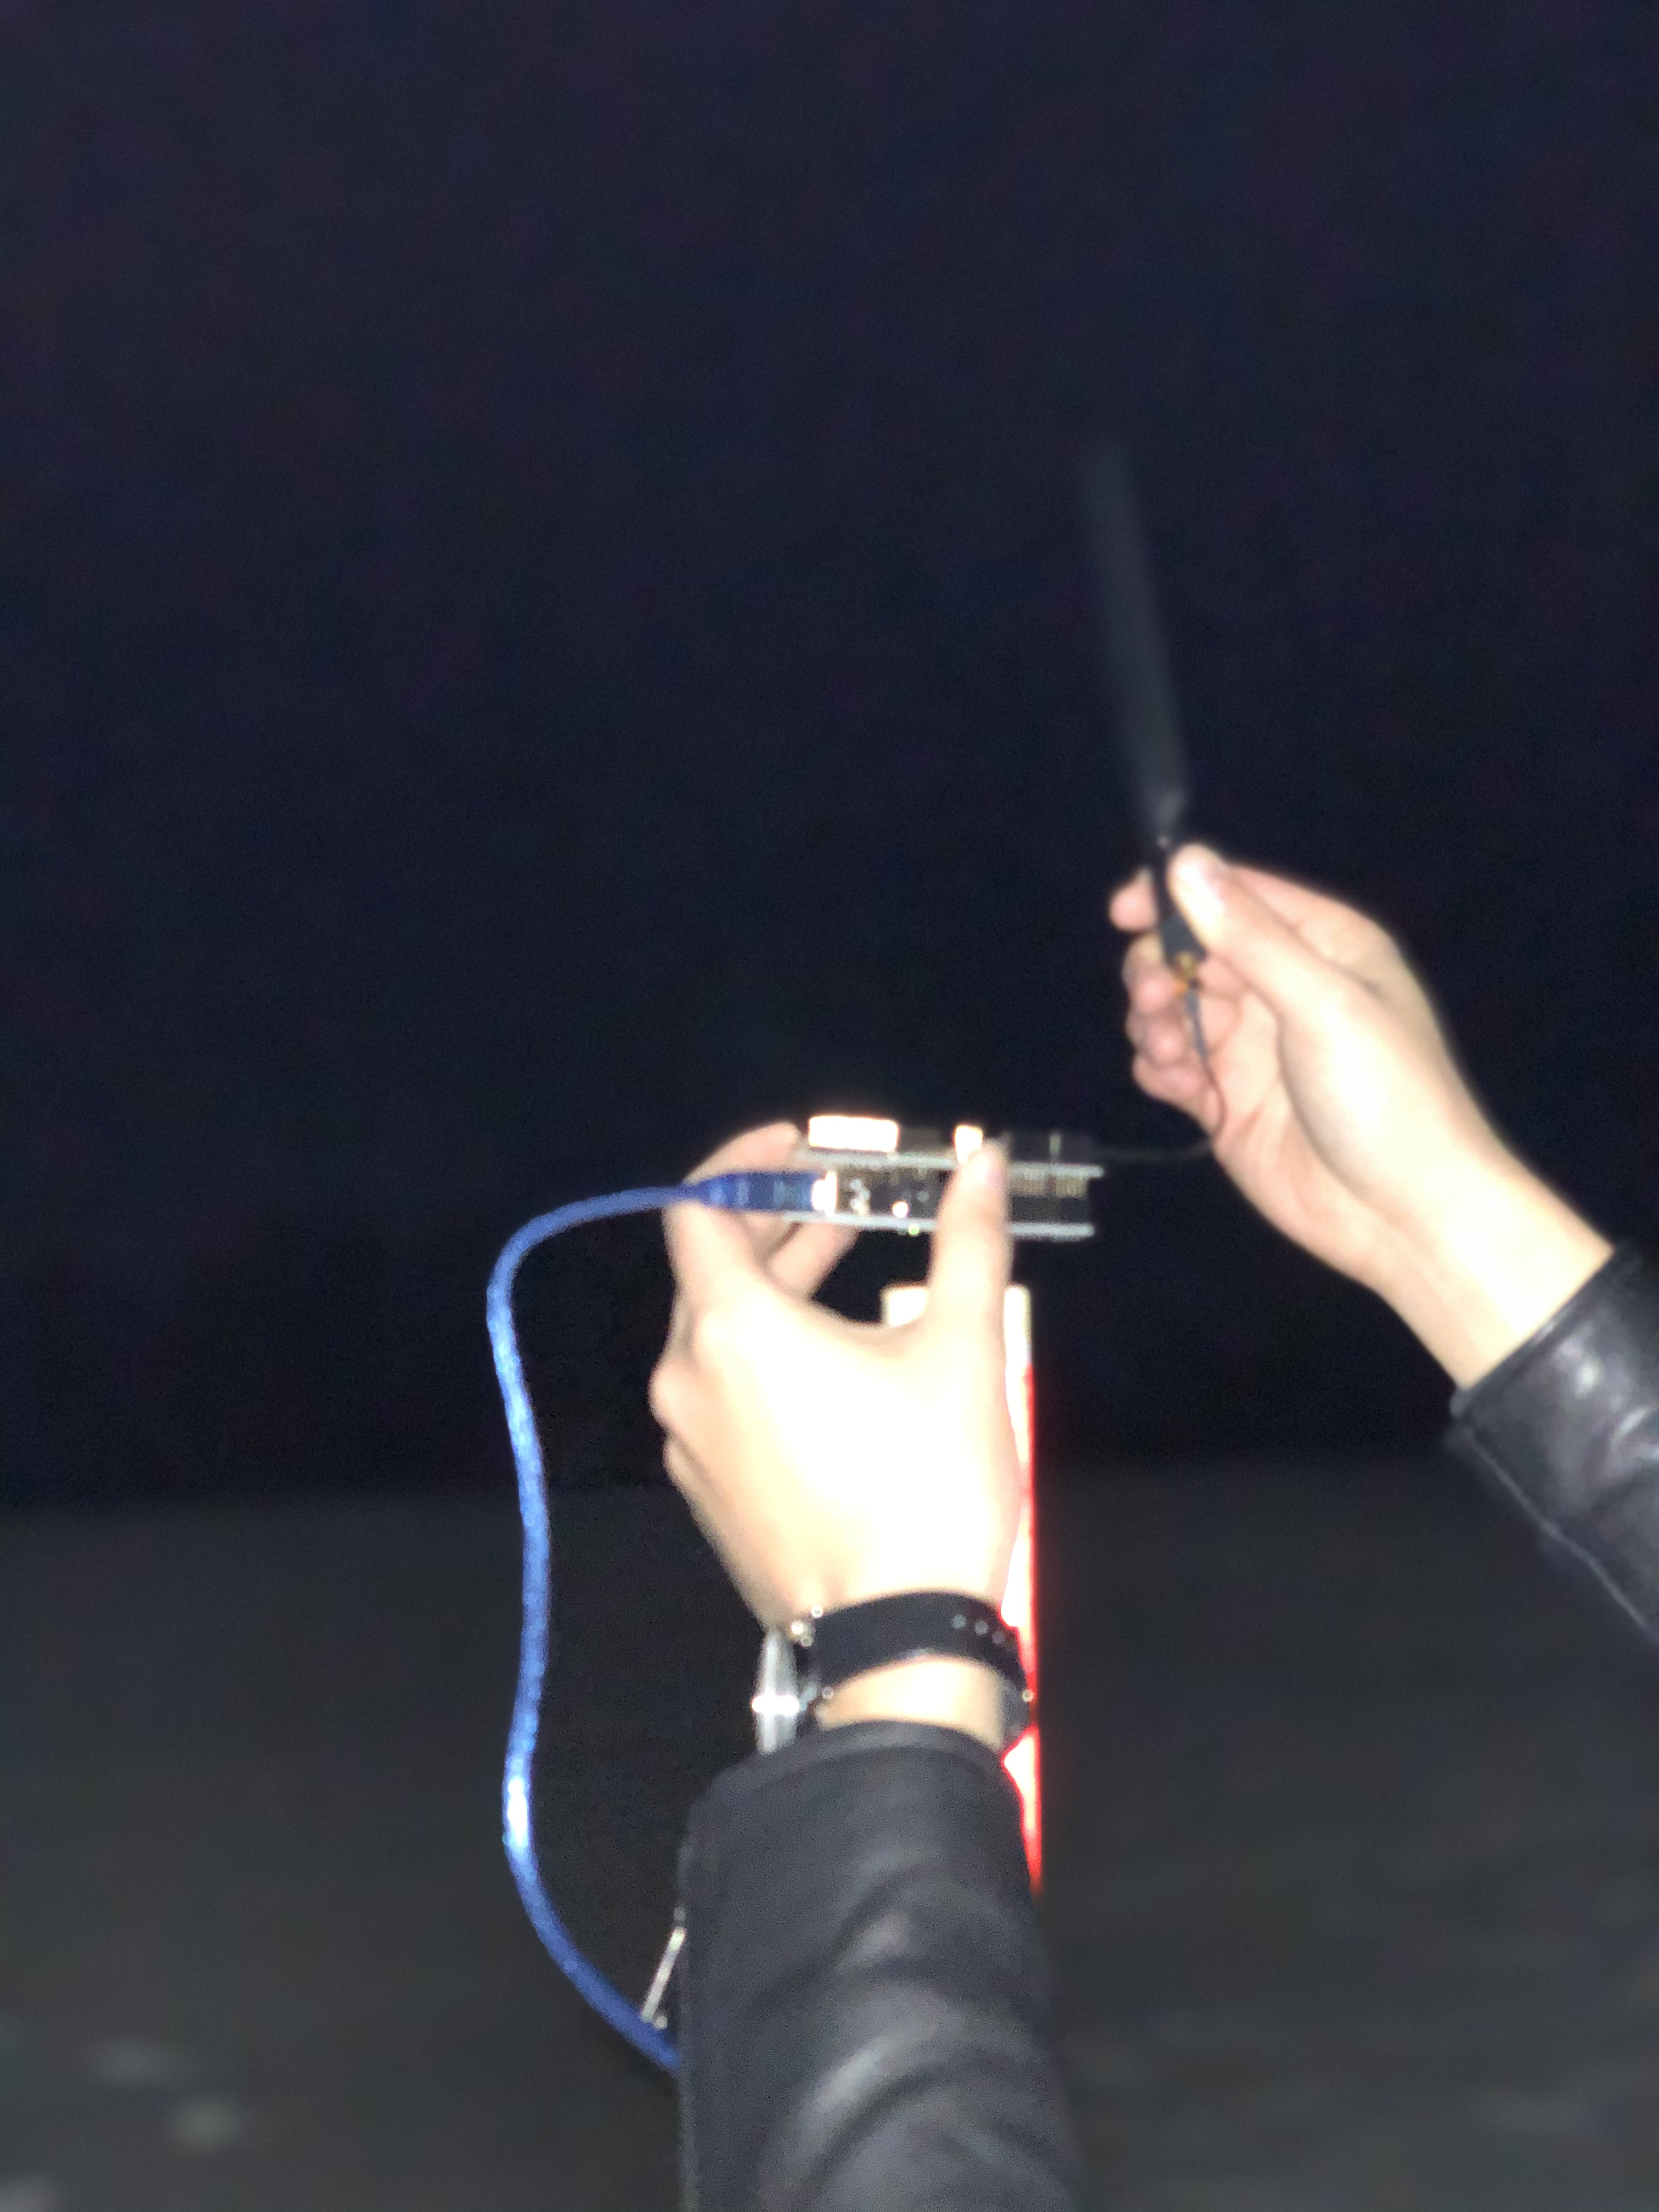
\includegraphics[width=5cm]{figures/experiment.jpg}
    \caption{実測実験の様子}
    \label{fig:experiment}
    \end{center}
\end{figure}

% ----
\section{実験結果}
LoRaWAN (DR2)でのイベントごとの消費電力実測結果を下記(表\ref{fig:result_power_consumtion}参照)(表\ref{fig:LoRaWAN_PowerConsumption}参照)に示す.また,LoRaWAN (DR2)でのその他値を下記(表\ref{fig:LoRaWAN_Parameter}参照)に示す.パケット到達率は,LoRaWANの送信回数に対してMQTTブローカーで受信したデータ数をもとに算出した.RSSiは,LoRaWANのGWノードが収集しMQTTブローカーに送信するため,その値を参考とした.SNRも同様である.

\begin{figure}[]
    \begin{center}
    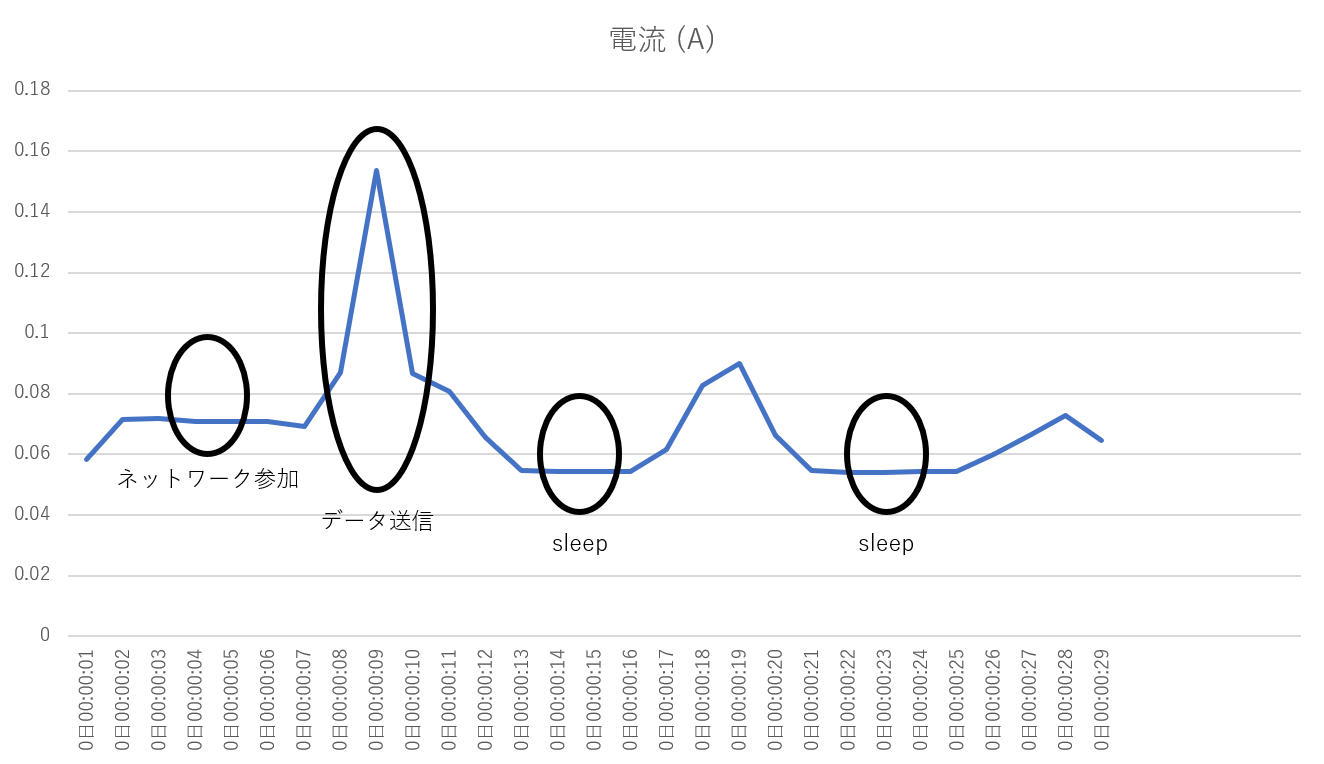
\includegraphics[width=15cm]{figures/LoRaWAN_消費電力実験.png}
    \caption{消費電力測定における各イベント(縦軸:消費電流,横軸:時間(s))}
    \label{fig:result_power_consumtion}
    \end{center}
\end{figure}

\begin{table}[]
    \caption{イベントごとの消費電力}\label{fig:LoRaWAN_PowerConsumption}
    \centering
    \begin{tabular}{|c|l|l|l|}
    \hline
    \textbf{イベント}     & \multicolumn{1}{c|}{\textbf{時間 (second)}} & \multicolumn{1}{c|}{\textbf{電流 (mA)}} & \multicolumn{1}{c|}{\textbf{消費電力 (mW)}} \\ \hline
    起動→ネットワーク参加       & 7                                         & 20                                    & 120                                     \\ \hline
    起動→ネットワーク参加→データ送信 & 11                                        & 21                                    & 105                                     \\ \hline
    スリープ              & なし                                        & 3                                     & 15                                      \\ \hline
    データ送信             & 4                                         & 29                                    & 145                                     \\ \hline
    \end{tabular}
\end{table}

\begin{table}[]
    \caption{その他パラメータ}\label{fig:LoRaWAN_Parameter}
    \centering
    \begin{tabular}{|c|c|}
    \hline
    \textbf{パラメータ} & \textbf{値} \\ \hline
    パケット到達率        & 90\%       \\ \hline
    RSSi           & -102       \\ \hline
    SNR            & -10        \\ \hline
    \end{tabular}
\end{table}
% % --- まとめ ---
% \chapter{実測に基づくグループ化アルゴリズムの適応点の評価}

\section{実験目的}
% 何を評価するために何を測って,どうなるとOKか,まで書いてください.
前項5.1.3(グループ化アルゴリズムの適応点の検討)で述べたように,グループ化の適応点を明らかにするため,LoRaWANにおける消費電力の実測を行う.適応点の評価については,前述したLoRaWANの既存方式と提案手法における関係式5.3に,実測した値を代入することで判断する.

\section{実験方法}
提案システムにおける各シーケンスにおいて消費電力を求めるため,起動からネットワーク参加,起動からネットワーク参加・初回送信,定常時の送信,スリープとイベントごと消費電力を計測する必要がある.実験では,市販のArduino互換LoRaWANモジュール及び消費電力計を用いて,消費電力を計測した.実験環境は,下記の表に示す.実験機材は,LoRaWANの送信機に,シングルボードコンピューターであるArduino Uno R3(表\ref{fig:Arduino_Spec}参照),LoRaWAN Shield for Arduino\cite{lorashield}(表\ref{fig:LoRaWAN_Spec}参照),受信機にLoRaWAN Gateway\cite{loragateway}(表\ref{fig:LoRaWAN_Gateway_Spec}),消費電力測定にマルチメータ\cite{kotomi}(表\ref{fig:Kotomi_Spec}参照)を用いた.LoRaWANは長距離伝送がユースケースであるため,LoRaWANのノードとGWノードを,高低差があり,約3.5kmの距離がある公立はこだて未来大学と自宅間に配置した.また計測結果を保存できる容量に限りがあるため,3試行を1セットとした.LoRaWANの設定内容を述べる.前述したLoRaWANのADR機能を適応し,スリープ時間は4秒とした.30秒間の計測を4セット12試行した.パケット到達率を算出するため,データ受信を確認する必要がある.本実測で利用したLoRaWANモジュールのプロバイダーは,MQTT ブローカーが提供しているため,MQTT クライアント\cite{mqtttool}を用いてデータを取得した.下記(図\ref{fig:experiment}参照)は,実験の様子である.

\begin{table}[]
    \caption{ARDUINO UNO REV3}\label{fig:Arduino_Spec}
    \centering
    \begin{tabular}{|c|c|}
    \hline
    動作電圧     & 5V   \\ \hline
    DC電流     & 50mA \\ \hline
    フラッシュメモリ & 32KB \\ \hline
    SRAM     & 2KB  \\ \hline
    EEPROM   & 1KB  \\ \hline
    \end{tabular}
\end{table}

\begin{table}[]
    \caption{LoRaWAN Shield for Arduino}\label{fig:LoRaWAN_Spec}
    \centering
    \begin{tabular}{|c|c|}
    \hline
    電源電圧 & DC2.2 $\sim$3.6V      \\ \hline
    周波数  & 920.6MHz $\sim$928MHz \\ \hline
    動作温度 & 0°C $\sim$40 °C       \\ \hline
    サイズ  & 68mm×53mm × 22.8mm    \\ \hline
    無線規格 & LoRaWAN 1.0.2         \\ \hline
    \end{tabular}
\end{table}

\begin{table}[]
    \caption{Kotomi Premium}\label{fig:Kotomi_Spec}
    \centering
    \begin{tabular}{|l|l|}
    \hline
    サイズ    & 77 x 35 x 13mm \\ \hline
    ディスプレイ & 1.44インチ        \\ \hline
    電圧精度   & 0.0001V        \\ \hline
    電流制度   & 0.0001A        \\ \hline
    電圧範囲   & 3.7~25V        \\ \hline
    電流範囲   & 0~5A           \\ \hline
    \end{tabular}
\end{table}

\begin{table}[]
    \caption{LoRaWAN Gateway}\label{fig:LoRaWAN_Gateway_Spec}
    \centering
    \begin{tabular}{|c|c|}
    \hline
    モデル名         & SW-GW01                       \\ \hline
    チャンネル数       & 最大8ch                         \\ \hline
    Wireless LAN & 802.11 b/g/n 2.4G             \\ \hline
    送信出力         & 20mW (最大13 dBm)               \\ \hline
    受信感度         & Down to -142 dBm              \\ \hline
    動作温度         & -10ºC $\sim$55ºC              \\ \hline
    電源電圧         & DC 5V / 2A(ミニUSBポート経由)        \\ \hline
    インターフェース     & Ethernet x 1ポート, 3/4G USBドングル \\ \hline
    サイズ          & L:116 x W:91 x H:27 mm        \\ \hline
    重量           & 160g                          \\ \hline
    \end{tabular}
\end{table}

\begin{table}[]
    \caption{実測に用いた電源}\label{fig:LoRaWAN_Battery}
    \centering
    \begin{tabular}{|c|c|}
    \hline
    サイズ     & 72 x 70 x 31 (mm) \\ \hline
    重量      & 189g              \\ \hline
    バッテリー容量 & 5000mAh           \\ \hline
    入力      & 5V=2A             \\ \hline
    出力      & 5V=3A             \\ \hline
    \end{tabular}
\end{table}

\begin{figure}[]
    \begin{center}
    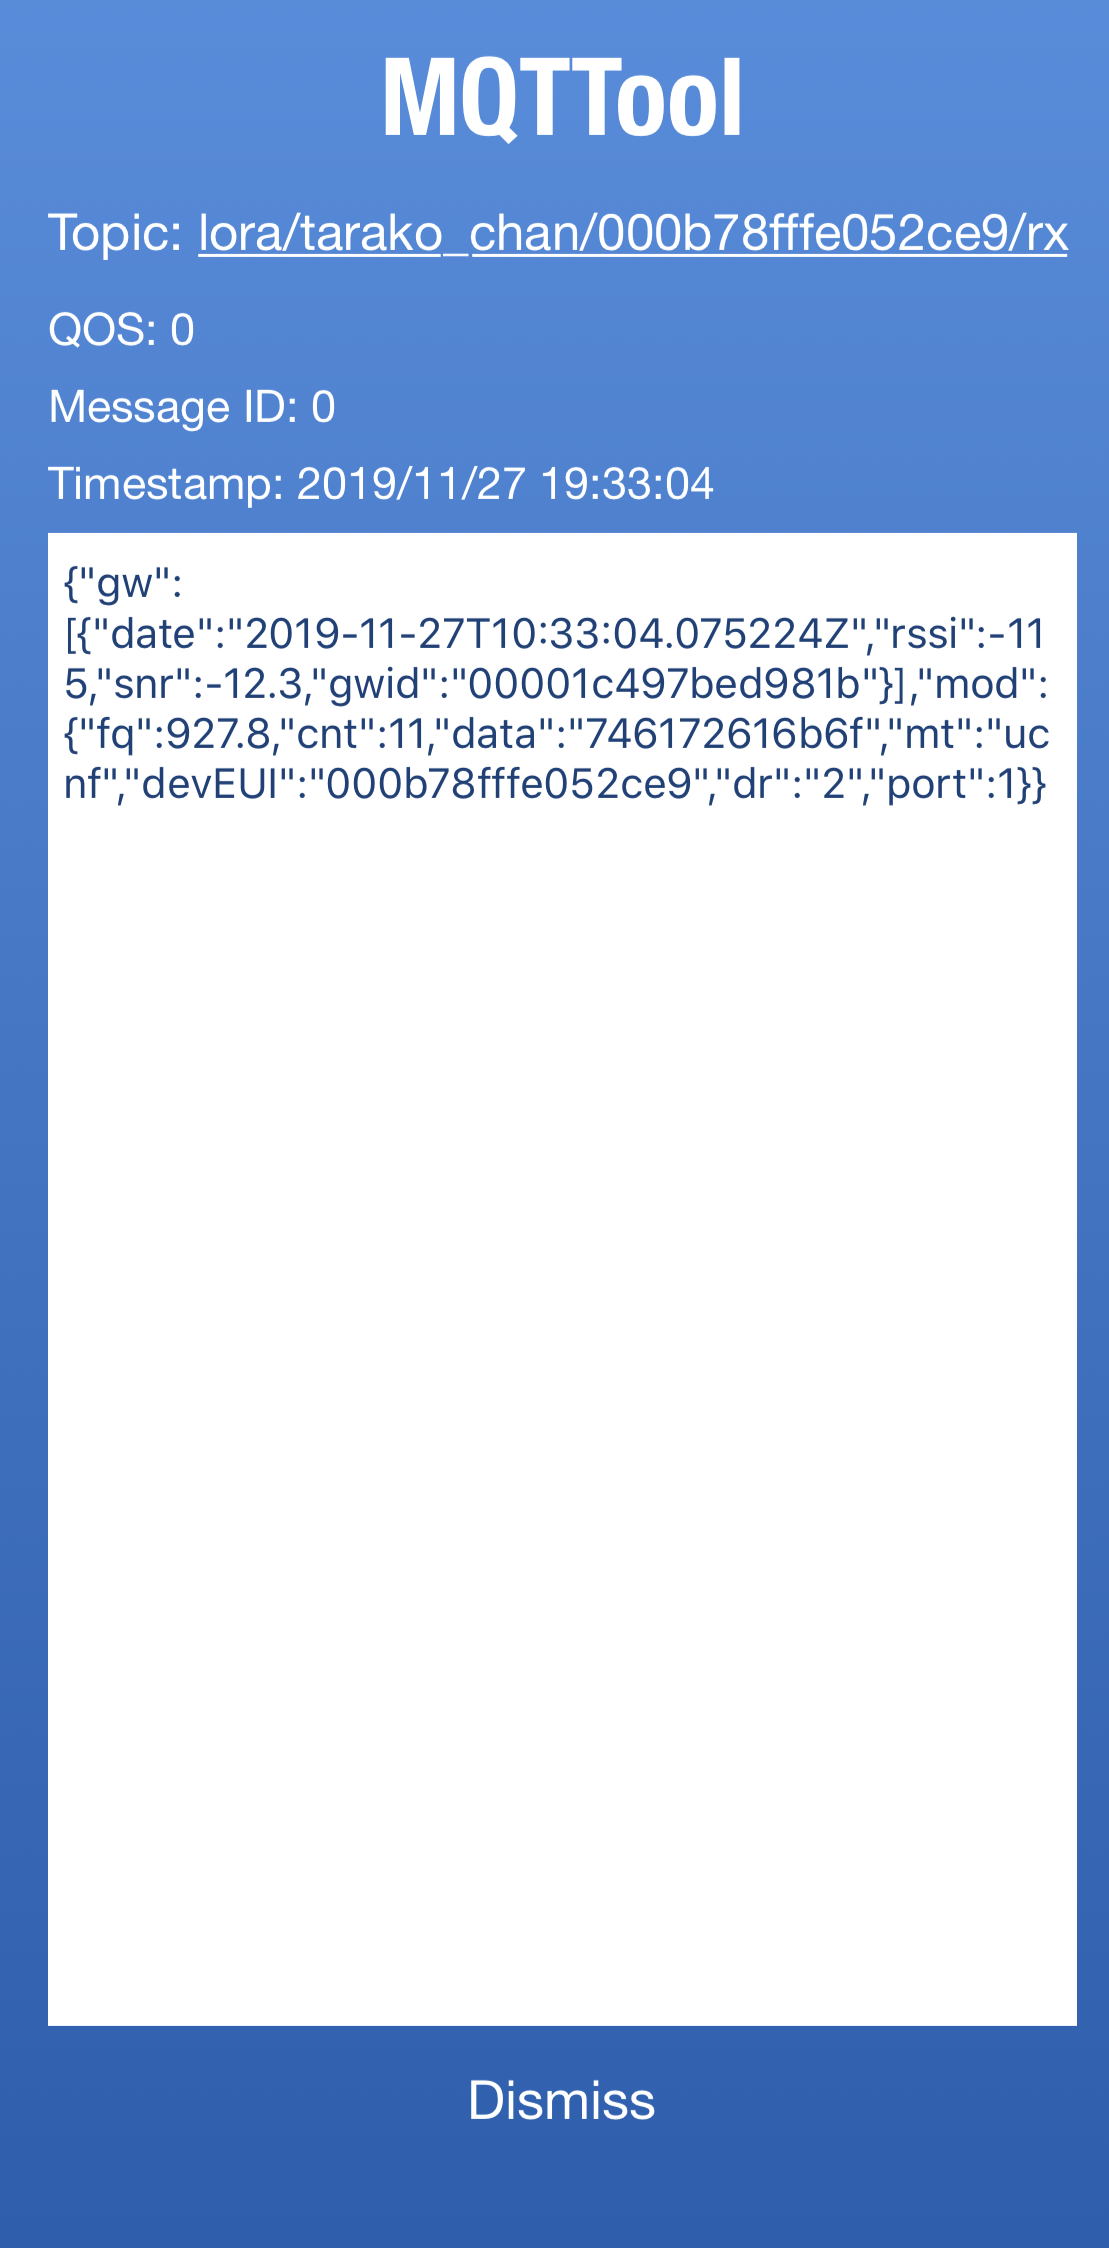
\includegraphics[width=5cm]{figures/mqtt.PNG}
    \caption{MQTT Client}
    \label{fig:mqtt}
    \end{center}
\end{figure}

\begin{figure}[]
    \begin{center}
    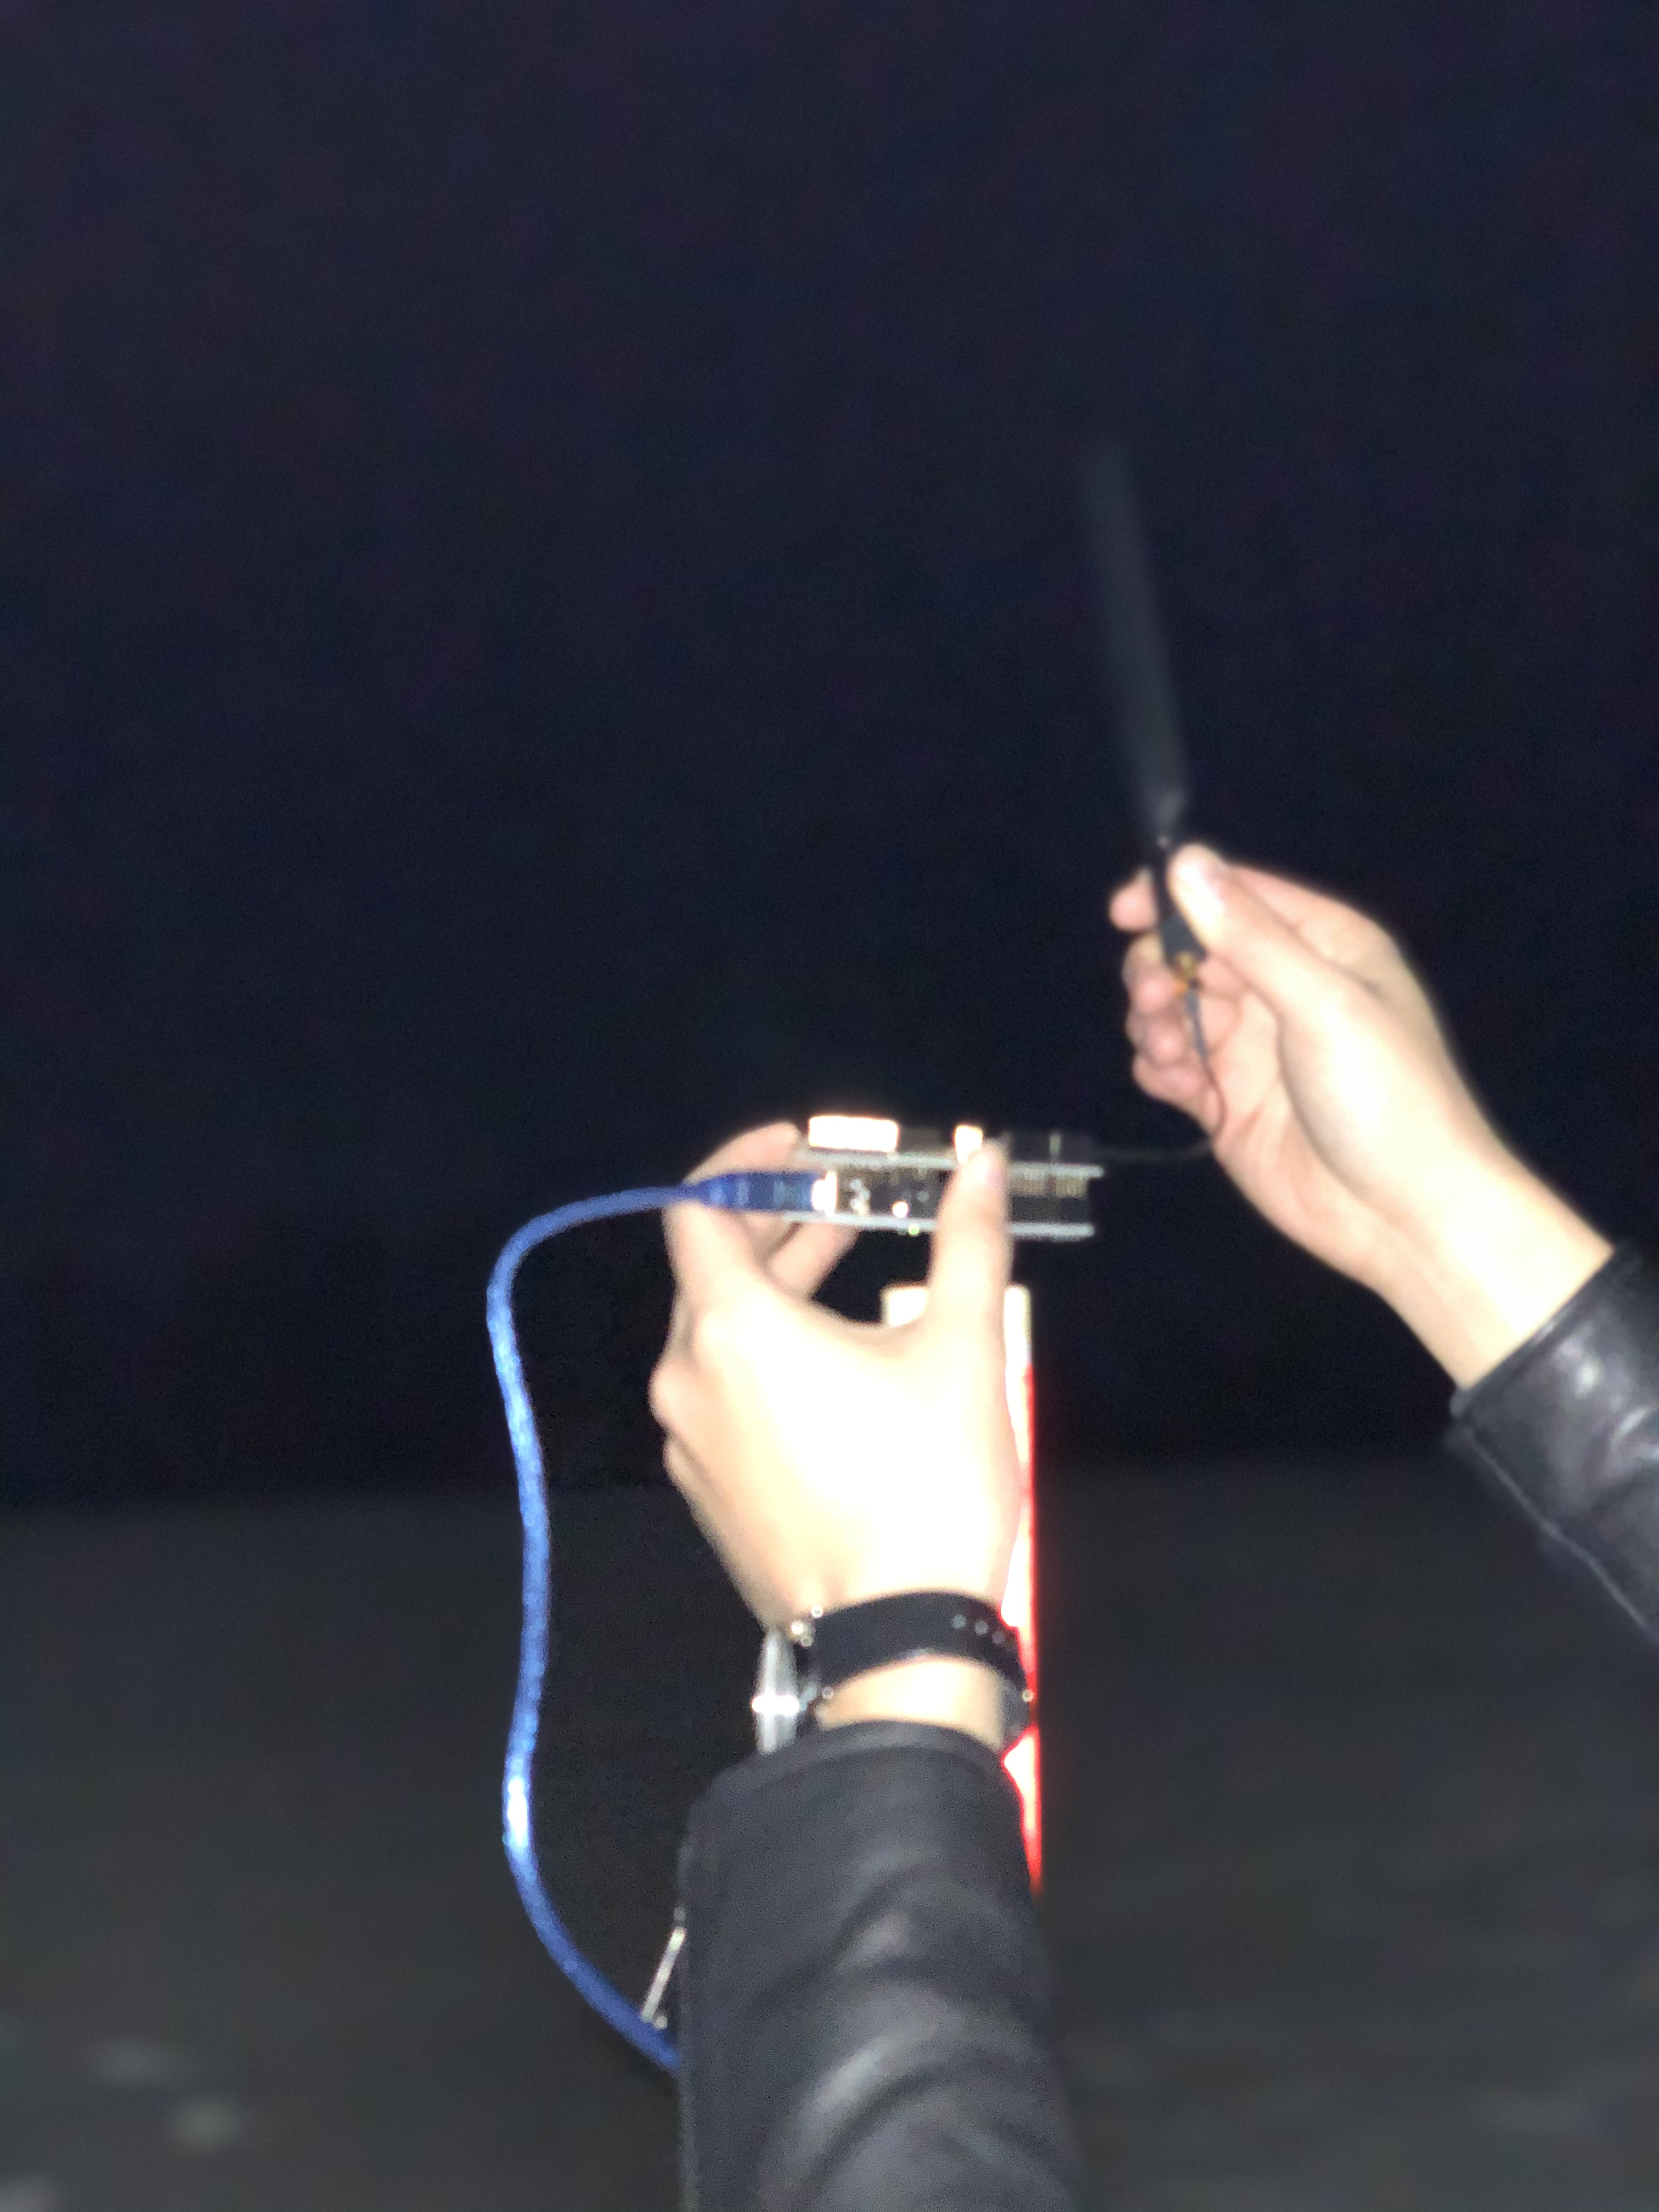
\includegraphics[width=5cm]{figures/experiment.jpg}
    \caption{実測実験の様子}
    \label{fig:experiment}
    \end{center}
\end{figure}

% ----
\section{実験結果}
LoRaWAN (DR2)でのイベントごとの消費電力実測結果を下記(表\ref{fig:result_power_consumtion}参照)(表\ref{fig:LoRaWAN_PowerConsumption}参照)に示す.また,LoRaWAN (DR2)でのその他値を下記(表\ref{fig:LoRaWAN_Parameter}参照)に示す.パケット到達率は,LoRaWANの送信回数に対してMQTTブローカーで受信したデータ数をもとに算出した.RSSiは,LoRaWANのGWノードが収集しMQTTブローカーに送信するため,その値を参考とした.SNRも同様である.

\begin{figure}[]
    \begin{center}
    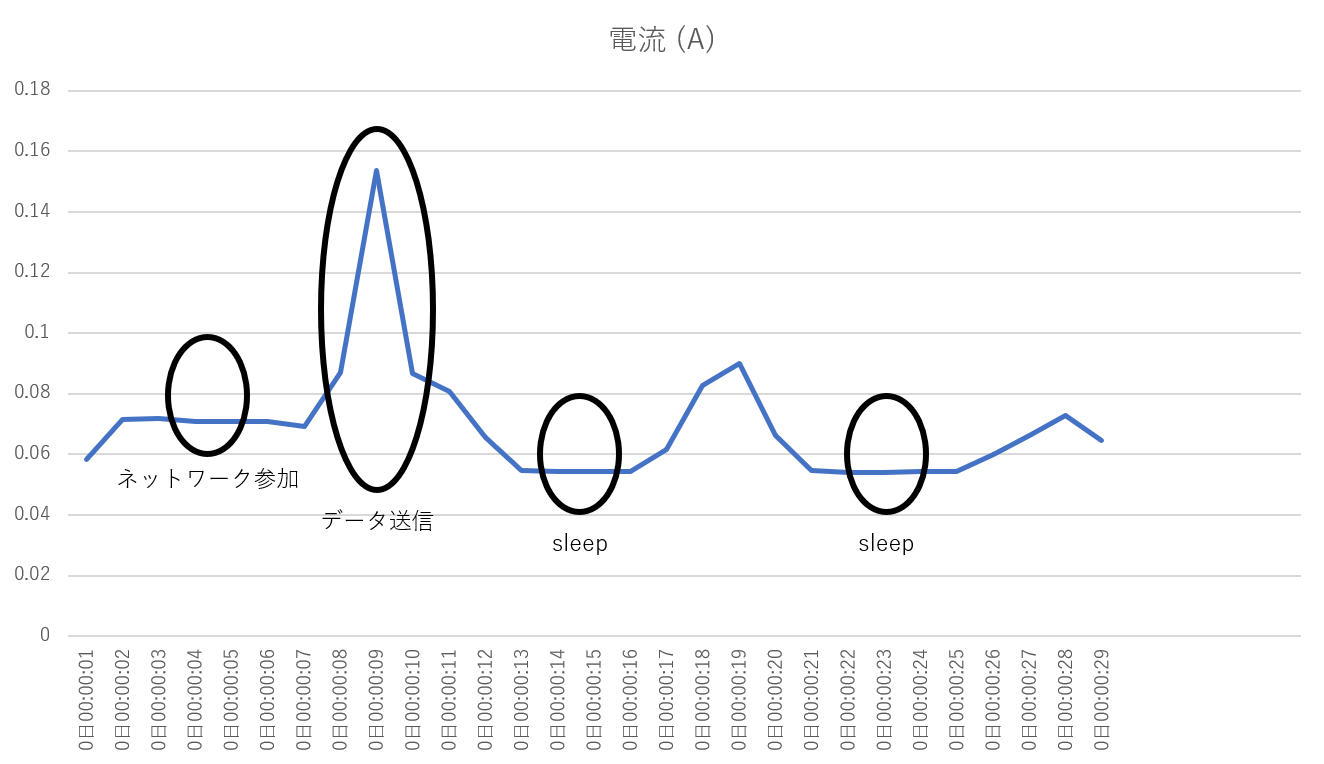
\includegraphics[width=15cm]{figures/LoRaWAN_消費電力実験.png}
    \caption{消費電力測定における各イベント(縦軸:消費電流,横軸:時間(s))}
    \label{fig:result_power_consumtion}
    \end{center}
\end{figure}

\begin{table}[]
    \caption{イベントごとの消費電力}\label{fig:LoRaWAN_PowerConsumption}
    \centering
    \begin{tabular}{|c|l|l|l|}
    \hline
    \textbf{イベント}     & \multicolumn{1}{c|}{\textbf{時間 (second)}} & \multicolumn{1}{c|}{\textbf{電流 (mA)}} & \multicolumn{1}{c|}{\textbf{消費電力 (mW)}} \\ \hline
    起動→ネットワーク参加       & 7                                         & 20                                    & 120                                     \\ \hline
    起動→ネットワーク参加→データ送信 & 11                                        & 21                                    & 105                                     \\ \hline
    スリープ              & なし                                        & 3                                     & 15                                      \\ \hline
    データ送信             & 4                                         & 29                                    & 145                                     \\ \hline
    \end{tabular}
\end{table}

\begin{table}[]
    \caption{その他パラメータ}\label{fig:LoRaWAN_Parameter}
    \centering
    \begin{tabular}{|c|c|}
    \hline
    \textbf{パラメータ} & \textbf{値} \\ \hline
    パケット到達率        & 90\%       \\ \hline
    RSSi           & -102       \\ \hline
    SNR            & -10        \\ \hline
    \end{tabular}
\end{table}
% % 以下必要に応じてchapterX.texを作成してinput文を記入

% % TODO: 謝辞
% \pagestyle{plain}
\chapter*{謝辞}
% TODO: 謝辞を以下に記入

謝辞を記入する.


% % TODO: 発表等実績
% % \chapter*{発表・採録実績}

% TODO: 発表・採録実績(確定分も含む)を以下の例のように記入

\subsection*{発表等}
\begin{enumerate}
\renewcommand{\labelenumi}{[\arabic{enumi}]}
    \item 情報処理学会 第82回全国大会(2020年3月)
\end{enumerate}

% % TODO: 参考文献
% \bibliographystyle{unsrt}
% \nocite{*}
% \bibliography{thesis}
% % TODO: 付録.必要がなければ削除すること
% \appendix
% \chapter*{付録}	% TODO: 章題を記入.題は任意.
\thispagestyle{plain}   % chapterの直後に必ず指定

%TODO: 章の内容を記入.以下はサンプル.
プログラムのソースリスト,その他関連資料などを,【必要があれば】載せる.
必要ない場合は,このページごと削除すること.
\TeX の場合は main.tex 内の \yen appendix 以下の2行を削除(またはコメント化)すればよい.
Wordの場合は前のページの「改ページ」以降を削除すればよい.
 

% % 図表一覧等自動生成
% \listoffigures
% \thispagestyle{plain}
% \listoftables
% \thispagestyle{plain}


\end{document}
